% Plan:
%
% Spis treści
% Spis rysunków
% Słowniczek skrótów
%
% Wstęp (1-2 strony): geneza, obszar, zawartość, dokonania autorów, opis struktury pracy
%
% Rozdziały merytoryczne (4-5, zrównoważone objętościowo):
%   Preambuła (ok. 0.5 strony)
%   Punkty merytoryczne (4-6)
%   Podsumowanie rozdziału
%
%   * opis technologii i uzasadnienie wyboru do rozwiązania problemu
%   * analiza wymagań + projekt systemu (architektura)
%   * opis implementacji, sposób uruchomienia
%   * badania eksperymentalne (tutaj także: profiling, opóźnienia)
%
% Podsumowanie pracy / Zakończenie
%   Wnioski końcowe
%   Co się udało / nie udało (+dlaczego!)
%   Możliwości rozwoju
%
% Spis literatury (numerowany, w tekście _muszą_ być odniesienia, ~20 pozycji)
%
%
% INNE:
%   * całość - ok. 60-70 stron
%   * numeracja - nie więcej, niż 3-poziomowa


\documentclass[11pt,openany]{book}
\usepackage[top=3cm, bottom=4cm]{geometry}
\usepackage[usenames,dvipsnames]{color}


% \usepackage[polish]{babel}
\usepackage[utf8]{inputenc}
\usepackage[T1]{fontenc}
\usepackage{fullpage}
\usepackage{fancyhdr}
\usepackage[pdfborder={0 0 0}]{hyperref}
\usepackage{float}
\usepackage{graphicx}
\usepackage{scrtime}
\usepackage{tabularx}
\usepackage{listings} 
\usepackage{caption}
\usepackage{color}
\usepackage{hyperref}
\usepackage{subfig}
\usepackage{tikz}
% \usepackage{pgf-umlsd}
\usepackage{tikz-uml}
\usepackage{todonotes}
\usepackage[acronym]{glossaries}
\usetikzlibrary{positioning,chains,fit,scopes}

% listings settings
\lstset{captionpos=b,frame=single,tabsize=2}

% include TikZ styles
\tikzstyle{terminal}=[
  rectangle,
  minimum size=6mm, rounded corners=3mm,
  very thick,
  draw=black!50,
  top color=white,bottom color=black!20,
  font=\ttfamily
]



% include Acronyms
\newacronym{acr:aac}{AAC}{Advanced Audio Coding}
\newacronym{acr:api}{API}{Application Programming Interface}
\newacronym{acr:atm}{ATM}{Asynchronous Transfer Mode}
\newacronym{acr:cir}{CIR}{Committed Information Rate}
\newacronym{acr:cm4j}{CM4J}{Crossbow Module for JIMS}
\newacronym{acr:cos}{CoS}{Class of Service}
\newacronym{acr:crud}{CRUD}{Create, Read, Update and Delete}
\newacronym{acr:dscp}{DSCP}{Differentiated Services Code Point}
\newacronym{acr:garp}{GARP}{Generic Attribute Registration Protocol}
\newacronym{acr:gui}{GUI}{Graphical User Interface}
\newacronym{acr:gvrp}{GVRP}{GARP VLAN Registration Protocol}
\newacronym{acr:haas}{HaaS}{Hardware as a Service}
\newacronym{acr:http}{HTTP}{Hypertext Transfer Protocol}
\newacronym{acr:iaas}{IaaS}{Infrastructure as a Service}
\newacronym{acr:ietf}{IETF}{Internet Engineering Task Force}
\newacronym{acr:ip}{IP}{Internet Protocol}
\newacronym{acr:isp}{ISP}{Internet Service Provider}
\newacronym{acr:it}{IT}{Information Technology}
\newacronym{acr:jims}{JIMS}{JMX-based Infrastructure Monitoring System}
\newacronym{acr:jmx}{JMX}{Java Management Extensions}
\newacronym{acr:jna}{JNA}{Java Native Access}
\newacronym{acr:jni}{JNI}{Java Native Interface}
\newacronym{acr:jvm}{JVM}{Java Virtual Machine}
\newacronym{acr:lan}{LAN}{Local Area Network}
\newacronym{acr:ldom}{LDOM}{Logical Domains}
\newacronym{acr:lxc}{LXC}{Linux Containers}
\newacronym{acr:mac}{MAC}{Media Access Control}
\newacronym{acr:mlet}{MLet}{Management applet}
\newacronym{acr:mvrp}{MVRP}{Multiple VLAN Registration Protocol}
\newacronym{acr:nfs}{NFS}{Network File System}
\newacronym{acr:nic}{NIC}{Network Interface Controller}
\newacronym{acr:osi}{OSI}{Open Systems Interconnection}
\newacronym{acr:paas}{PaaS}{Platform as a Service}
\newacronym{acr:phb}{PHB}{Per-Hop Behaviour}
\newacronym{acr:qos}{QoS}{Quality of Service}
\newacronym{acr:rfc}{RFC}{Request for Comments}
\newacronym{acr:rsvp}{RSVP}{Resource Reservation Protocol}
\newacronym{acr:rtp}{RTP}{Real-time Transport Protocol}
\newacronym{acr:s3}{S3}{SOA Solution Stack}
\newacronym{acr:saas}{SaaS}{Software as a Service}
\newacronym{acr:soa}{SOA}{Service-oriented Architecture}
\newacronym{acr:ssh}{SSH}{Secure Shell}
\newacronym{acr:swt}{SWT}{Standard Widget Toolkit}
\newacronym{acr:udp}{UDP}{User Data Protocol}
\newacronym{acr:vlan}{VLAN}{Virtual Local Area Network}
\newacronym{acr:vnic}{VNIC}{Virtual Network Interface Controller}
\newacronym{acr:vod}{VOD}{Video on Demand}
\newacronym{acr:voip}{VoIP}{Voice over Internet Protocol}
\newacronym{acr:vpls}{VPLS}{Virtual Private LAN Service}
\newacronym{acr:vrf}{VRF}{Virtual Routing and Forwarding}


\makeglossaries


\title{Component-based system for management of multilevel virtualization of networking resources}
\author{Robert Boczek \and Dawid Ciepliński}

% \department{Electrical and Computer Engineering}
% \school{AGH UNIVERSITY OF SCIENCE AND TECHNOLOGY}
% \degree{MSc Thesis}

%\address{Houston, Texas}
%\donemonth{September} \doneyear{2011} \makeindex

%\committee {
 %       Supervisor:  prof. dr hab. inż. Krzysztof Zieliński  \\
  %      Technical supervisor: mgr inż. Marcin Jarząb
%}

\date{\today}

\renewcommand{\headrulewidth}{0pt}

\begin{document}

  \newcommand{\makethesistitle}[7]
  {
    \thispagestyle{fancy}
    \cfoot{Kraków 2011}

    \begin{center}

      {\huge #1}

      \rule{\textwidth}{.15ex}

      {\large #2}

      \medskip

      \textsc{\large #3}

      \vspace{1cm}

      
\includegraphics{img/agh-logo.pdf}

      \vspace{1cm}

      \textsc{\LARGE #4}

      \vspace{1.5cm}

      \textsc{\Large Robert Boczek, Dawid Ciepliński}

      \vspace{1.5cm}

      \textsc{\textbf{\Large #5}}

    \end{center}

    \vspace{2cm}

    \begin{tabularx}{\textwidth}{Xl}
      & \textsc{#6:} \\
      & prof. dr hab. inż. Krzysztof Zieliński \\
      & \\
      & \textsc{#7:} \\
      & mgr inż. Marcin Jarząb
    \end{tabularx}

    \newpage
  }

  \listoftodos\newpage

  \makethesistitle{Akademia Górniczo-Hutnicza \\ \vspace{1ex} im. Stanisława Staszica}
                  {Wydział Elektrotechniki, Automatyki, Informatyki i Elektroniki}
                  {Katedra Informatyki}
                  {Praca Magisterska}
                  {System komponentowy wspomagający zarządzanie \\ wielopoziomową wirtualizacją zasobów sieciowych}
                  {Promotor}
                  {Opiekun techniczny}

  {\thispagestyle{empty}

    ~

    \vfill

    \hfill
    \begin{tabular*}{.75\textwidth}{p{.75\textwidth}}
      Oświadczamy, świadomi odpowiedzialności karnej za poświadczenie nieprawdy, że niniejszą pracę dyplomową
      wykonaliśmy osobiście i~samodzielnie (w zakresie wyszczególnionym we wstępie) i~że nie korzystaliśmy ze źródeł
      innych niż wymienione w pracy.
    \end{tabular*}

    \vspace{2cm}

    \hfill
    \begin{tabular}{c}
      \ldots\ldots\ldots\ldots\ldots\ldots\ldots \\
      podpis                                     \\
                                                 \\
      \ldots\ldots\ldots\ldots\ldots\ldots\ldots \\
      podpis
    \end{tabular}

    \newpage
  }

  \makethesistitle{AGH \\ \vspace{1ex} University of Science and Technology}
                  {Faculty of Electrical Engineering, Automatics, Computer Science and Electronics}
                  {Department of Computer Science}
                  {Master of Science Thesis}
                  {Component-based system for management of \\ multilevel virtualization of networking resources}
                  {Supervisor}
                  {Technical supervisor}

	\vspace*{2in}

	\begin{center}
    \textit{We would like to acknowledge the support and assistance given us by professor~Krzysztof~Zieliński and
            Marcin~Jarząb. Their generously contributed ideas, feedback and advice was of great help to us. \\
            Finally, we would like to thank our families and friends for their support and encouragement.}
  \end{center}

  \tableofcontents

  \listoffigures

  \newpage


  \chapter{Introduction}
  \label{chap:intro}

    In today's world every successful organisation is based on a properly designed communication networks. These networks
    must deal with delay-sensitive data such as real-time audio and video or other mission-critical data. Therefore,
    safe, predictable and, very often, guaranteed services have to be provided. Accomplishing the required \gls{acr:qos}
    by controlling delay, delay variation (jitter), bandwidth and packet loss parameters is a deeply hidden secret of most
    successful end-to-end business applications.
    
    Technologies like Ethernet did not foresee \todo[inline]{raczej nie byly zaprojektowane; chyba, ze damy zrodlo} the future
    necessity of providing \gls{acr:qos} therefore implementing \gls{acr:qos} solutions over the Internet is such a
    demanding issue. Incomplete resource reservation provided by most common operating systems induced further research
    in the field of resource reservation and isolation. 

    % http://www.cisco.com/en/US/products/ps6558/products\_ios\_technology\_home.html

    The increasing popularity of virtualization, isolation and resource reservation in contemporary systems encourages
    further research.

    \todo[inline]{napisac, gdzie wirtualizacja ma zastosowanie, oprocz grid i cloud}


    \section{Thesis objective}

      Having all the above facts taken into account the following thesis statement was proposed: \textit{There exists a
      component-based architecture which enables construction of a system that would facilitate working with a fully
      isolated virtualized network and resources grouped by project name.}

      Due to a substantial lack in similar products available on the market research in this area was planned. The main system
      responsibilities would be providing fast and efficient manner of creating any requested, virtualized network
      structure with virtualized resources, network elements and \gls{acr:qos} guarantees.  Solaris operating system is
      already a respectable solution in terms of resource virtualization. Recently supported by network virtualization
      mechanism contained in the Crossbow project, Solaris OS seems to be a suitable environment to proceed further
      research.

      The thesis objective is to design the architecture, implement it and verify using a series of tests.


    \section{Organization of the thesis}

      The remaining part of this paper is divided into seven chapters, each containing a description and discussion of
      particular stage of the system construction process.

      Chapter \ref{chap:bck} provides domain information about resource and network virtualization and supplying
      \gls{acr:qos} guarantees for \gls{acr:ip} networks. Virtual infrastructures are described
      together with an overview of technologies in common use.

      Chapter \ref{chap:req} introduces crucial definitions of objects and processes discussed throughout the paper.
      Based on these definitions and constraints imposed, functional requirements and qualities of the system are
      identified and presented.

      An overview of Solaris OS is presented in chapter \ref{chap:sol}. Special attention is paid to virtualizations
      mechanisms present in the environment and ways to manage resource consumption policies. Crossbow --- network
      virtualization subsystem --- is then described thoroughly.

      Suggested architecture of the system is introduced in chapter \ref{chap:arch}. The architecture is analyzed with
      respect to its two main layers --- instumentation and infrastructure --- designed to provide different levels of
      abstraction and fulfill the requirements of the system.

      Chapter \ref{chap:impl} discusses implementation details of the system. It also lists problems encountered while
      implementing the system together with chosen solutions. Integration with \gls{acr:jims} is described and system
      verification process is summarized.

      The scenario that was designed and executed to validate the operation of implemented system is examined in chapter
      \ref{chap:cs}. The case study, inspired by multimedia systems, allows to verify that most of functionalities of the
      system are implemented properly.

      Chapter \ref{chap:sum} summarizes research performed in the field of network virtualization. Achieved goals are
      described together with possible directions of further improvements and functionalities that may be welcomed.
      Finally, objectives that were not completed are listed.
      

    \section{Individual contributions}

      The thesis is a result of joint effort of the authors. However, there are areas where particular author
      contributed majority of the content. The division is listed in table \ref{tab:intro:contrib}.

      \newcommand{\compref}[1]{\ref{#1} \nameref{#1}}

      \begin{table}[h]
        \centering

        \begin{tabular}{|l|l|}
          \hline
          \multicolumn{1}{|c|}{Chapter} & \multicolumn{1}{c|}{Author}     \\
          \hline \hline
          \compref{chap:intro}          & Robert Boczek                   \\
          \hline
          \compref{chap:bck}            & Robert Boczek, Dawid Ciepliński \\
          \hline
          \compref{chap:req}            & Robert Boczek                   \\
          \hline
          \compref{chap:sol}            & Robert Boczek, Dawid Ciepliński \\
          \hline
          \compref{chap:arch}           & Dawid Ciepliński                \\
          \hline
          \compref{chap:impl}           & Robert Boczek                   \\
          \hline
          \compref{chap:cs}             & Dawid Ciepliński                \\
          \hline
          \compref{chap:sum}            & Robert Boczek, Dawid Ciepliński \\
          \hline
        \end{tabular}

        \caption{Individual contributions}
        \label{tab:intro:contrib}
      \end{table}


  \chapter{Technological background}
  \label{chap:bck}

    The chapter provides background information about the domain the created system manages as well as the environment
    it runs in. Fields of applications and advantages of using virtual infrastructures are described. Subsequently
    networking with various level of \gls{acr:qos} guarantees, overview of virtualization techniques together with
    technology examples and detailed discussion of networking virtualization is presented.

    Section \ref{sec:ctx:virt} introduces basic information about resource virtualization. The reasons why
    virtualization is essential in contemporary systems management are discussed. Then, resources that can be
    virtualized are listed together with common virtualization techniques.

    Section \ref{sec:ctx:multi} presents network virtualization methods. The definition of virtualized network is
    provided and the types of virtual networks are listed. Also, virtualization methods for network devices belonging to
    various layers of the \gls{acr:osi} model are described. The definition and application of virtual appliances to
    deploy services are discussed. Finally, the concept of ,,Network in a box'' --- encompassing virtualization, virtual
    appliances approach and \gls{acr:qos} --- is presented.

    Section \ref{sec:ctx:infra} enumerates some of possible applications of virtual network infrastructures. The section
    is focused on using the infrastructures to build complex test environments, providing scalable server-side solutions
    and the concept of \gls{acr:iaas} used in cloud computing. A separate subsection is dedicated to virtualization as
    one of the core components in \gls{acr:soa} and \gls{acr:s3} models.

    Section \ref{sec:ctx:qos} describes the problem of providing \gls{acr:qos} in computer networks of different types.
    The approaches chosen by \gls{acr:atm}, Token Ring and Frame Relay networks are outlined. The remaining part of the
    section discusses Differentiated~Services and Integrated~Services --- the solutions enabling \gls{acr:qos} in
    best-effort \gls{acr:ip} networks.

    % Constantly growing demand for bandwidth in networks (especially \gls{acr:vod}, \gls{acr:voip}, RT) raises the
    % question: 'Whether it is better to increase available bandwidth of networks or to build intelligent systems managing
    % users traffic?'. As high bandwidth is just not enough because there are other equally important transmission
    % parameters (delay, jitter, package missing	tolerance) there seems to be just one correct answer for this question.
    % Creating such systems is not an easy task and many groups such as \gls{acr:ietf} are working on this problem.
    % Currently there are three existing models performing \gls{acr:qos} in the \gls{acr:ip} network:

    % \begin{enumerate}
    %   \item best effort,
    %   \item Intserv,
    %   \item Diffserv.
    % \end{enumerate}

    % These models are discussed in more details in the following section.


    \section{Resource virtualization}
    \label{sec:ctx:virt}

      Resource virtualization is \todo[inline]{dajmy tu bardziej ogolna definicje} in principle separation application from
      physical hardware on which it runs. It also allows dividing single physical hardware to multiple virtualized
      logical resources, thereby running the software under virtualized resources lowers cost, improves efficiency,
      introduces isolation and better configurability. 


      \subsection{The need for virtualization}

        Together with increasing hardware evolution problems with its better utilization arose. Low fault tolerance, no
        isolation and poor utilization of available resources implicated the demand of creating an approach overcoming
        this issues. 

        It was not until 1960s that virtualization was first used for better hardware utilization of some large,
        mainframe hardware. Today, over 50 years later when computers got more common than ever problems of rigidity and
        underutilization are still present. Nowadays companies like VMWare invest more and more funds in research as
        they foresee that virtualization will become even more popular and common in the future \cite{virtualization}.


      %\subsection{Resources that can be virtualized} 

      \subsection{Common approaches}

        \todo[inline]{rozszerzyc - wiecej tekstu}

        In terms of approaches to resource virtualization, in principle there are three existing acknowledged
        approaches:

        \begin{itemize}
          \item{Full virtualization,}
          \item{Partial virtualization,}
          \item{OS-level virtualization.}
        \end{itemize}


      \subsection{Full virtualization}

        Full virtualization is a technological approach to virtualization also known as emulation of the underlying raw
        hardware (native execution). This approach may be implemented with two types of hypervisors. The first one runs
        directly on hardware, whereas the second one requires another operating system, such as Linux or Windows. There
        are no restrictions towards operating system being run --- it has to support the underlying hardware \todo[inline]{czy o
        to chodzilo?}.
        In terms of running different "guest" \todo[inline]{definicja!} operating systems together no limitations exist.

        By now, full virtualization approach implementations for x86 such as Virtual PC, VirtualBox exist and are ready
        to use. \todo[inline]{rozszerzyc ten akapit}


      \subsection{Partial virtualization}

        Also called emulation of a non-native system is based on allowing software applications written for different
        computer hardware architecture to startup. Virtual resource emulate hardware which exists based on detailed
        specification. Java virtual machine or 'Open firmware'\todo[inline]{definicja i zrodlo do tego}, that allows hardware to be run under any kind of CPU,
        are the most commonly used and known representatives of this approach to resource virtualization. \todo[inline]{jak sie
        da, to jasniej o tym, bo jest ciezkie do zrozumienia}


      \subsection{OS-level virtualization}

        Operating System-level virtualization is a technology consisting of virtualizing servers on an operating system
        layer.  Multiple guest operating systems may be running under the same host system, but these guest operating
        systems must be the same,
        although different libraries and distributions are allowed\todo[inline]{uproscic to zlozone zdanie}. OS-level virtualization may be often presented as
        slicing single OS to small partitions (sometimes called virtual environments (VE), virtual private servers (VPS)
        or zones). From the end-user perspective these virtualization is invisible (user receives guest OS as real
        server).

        \todo[inline]{przyklady!}


    \section{Multilevel network virtualization}
    \label{sec:ctx:multi}

      Network virtualization is based on providing separate networking environments for defined groups of users. For
      each group logical environments are created over single existing physical network infrastructure. These created
      networks provide complete network services so that from the end-user perspective dedicated network with policies
      and resources is available. Network virtualization concerns not only logical segmentation of the network
      transport, but also network devices and other network services \cite{network_virt}.

      The problem of networking resources virtualization is multifaceted. There are many aspects at various levels that
      should be considered --- virtualization at the Data Link Layer of the \gls{acr:osi} model, providing software
      equivalents of equipment used by higher network layers (e.g. virtual routers), or creating fully virtualized
      networks with \gls{acr:qos} guarantees. The section provides an overview of these techniques together with
      examples of technologies used.


      \subsection{Types of virtual networks}

        Virtualized networks belong to one of two main classes --- internal or external \cite{nsag}. Internal
        virtualization utilizes a single machine to create a logical network topology inside, whereas external
        virtualization means using existing physical infrastructure (comprising multiple nodes) to build subnetworks on
        top of it.

        As far as internal virtualization is considered, the main building blocks are virtual network interface cards
        and virtual switches. These components establish logical links between virtual appliances (counterparts of
        physical machines). Examples of internal virtualization solutions include Xen domains, VirtualBox internal
        networks \cite{vboxum} and Solaris Containers with Crossbow technology.

        External virtualization is implemented with Layer 2 switches aware of \gls{acr:vlan} technology. With these
        devices, entire network is split into fully-isolated parts, each becoming a new independent network. Routers can
        then be used to establish connectivity between selected subnetworks.

        The approaches listed can be interoperate to create hybrid topologies with some parts of a network using
        internal virtualization and some using external one. Figure \ref{fig:ctx:nvtypes} depicts an example of a
        network topology that uses both internal and external virtualization.
        
        \begin{figure}[H]
          \centering
          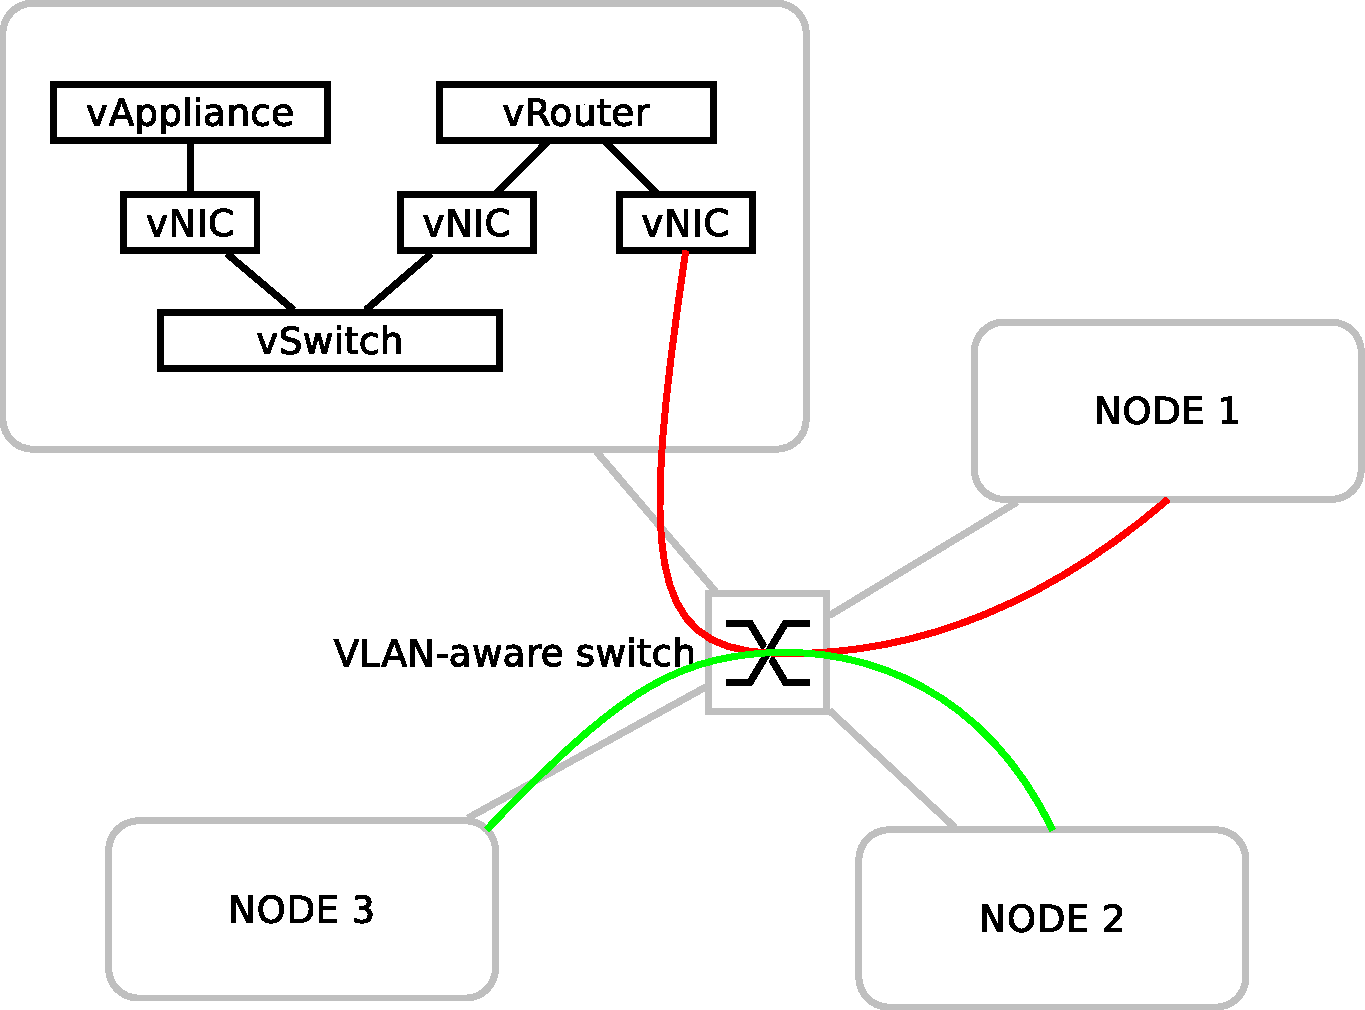
\includegraphics[width=.5\textwidth]{img/ctx/vnet-types.pdf}

          \caption{Internal and external network virtualization}
          \label{fig:ctx:nvtypes}
        \end{figure}


      \subsection{Virtualized network devices}

        Virtualized network devices (i.e. nodes used to build network paths between boundary machines providing or
        consuming services) include mostly those belonging to second and third layer of the \gls{acr:osi} model (e.g.
        switches and routers, respectively). However, devices that are assigned to higher layers are subject to
        virtualization, too.

        Two virtualization approaches can be distinguished: partitioning of physical devices in order to create logical
        entities with assigned resources or software-based solutions used to build independent virtualized components
        with the same behaviour as their physical counterparts. Both methods can be applied at various layers of the
        \gls{acr:osi} model. In the context of network devices, virtualization means creating both virtual as well as
        logical resources.

        Data Link layer virtual resources can be created --- these include virtual switches and virtual network
        interface cards built on top of them. Virtual routers connect network segments the same way as physical ones.
        More sophisticated examples include software implementations of firewalls and load balancers.

        Logical devices require specialized hardware and the approach is used mainly in high-end solutions.
        \gls{acr:vlan} technology is one of the most widely used partitioning techniques within Data Link layer ---
        ports of a switch are grouped to provide separate broadcast domains. Another technique, used to merge
        geographically distributed segments and create single Layer 2 segment is \gls{acr:vpls} \cite{moreno}.
        \gls{acr:vrf} is used to create logical routing entities on top of physical partitioning-capable routers.


      \subsection{Virtual appliances}
      \label{sub:}

        % ogolnie o podejsciu, przyklady
        % can serve various purposes - ordinary network nodes (app layer: workstations, servers, proxy?) but also
        % routers, firewalls, load balancers
        % IMPORTANT: often host a single application

        % Solaris Zones, together with other components of the Solaris OS, constitute a complete framework that
        % implements virtual appliance approach to systems management.

        Virtual appliance is a \textit{pre-built, pre-configured, ready-to-run (enterprise) application packaged along
        with an optimized operating system inside a virtual machine} \cite{changhua}. The main problem virtual
        appliances can solve is the complexity and duration of application deployment process.  In general, a service
        deployment can be described as comprising the following stages: preparation (learning the dependencies),
        pre-installation, installation and post-installation. With traditional (non-virtualized) approach, these stages
        have to be repeated every time a service is deployed on different machines.

        \begin{figure}[H]
          \begin{center}
            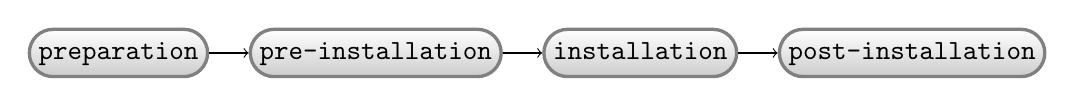
\begin{tikzpicture}[start chain,
                                node distance=5mm,
                                every node/.style={on chain, join, terminal},
                                every join/.style={->},
                                text depth=.25ex]

              \node {preparation};
              \node {pre-installation};
              \node {installation};
              \node {post-installation};
            \end{tikzpicture}
          \end{center}

          \caption{Traditional application deployment stages}
        \end{figure}

        Virtual appliance approach makes it possible to reduce deployment time significantly \cite{changhua}. This is
        achieved by performing most of the deployment stages once and storing the configured environment in a virtual
        appliance. The appliance can then be moved to publicly-available repository for actual deployment on host
        systems. Deployment process with virtual appliances leveraged is depicted in figure \ref{fig:sol:dep-va}

        \begin{figure}[H]
          \begin{center}
            \begin{tikzpicture}[node distance=5mm]

              { [start chain, every node/.style={terminal, on chain, join, text width=3cm}, every join/.style={->}, align=center]

                { [every on chain/.style={text width=3.5cm}, text depth=.25ex, align=center]

                  \node (prep)                 {preparation};
                  \node (pre)  [below=of prep] {pre-installation};
                  \node (ins)  [below=of pre]  {installation};
                  \node (post) [below=of ins]  {post-installation};
                }

                \node (pub)  [right=of post] {appliance publication};
                \node (act)  [right=of pub]  {appliance retrieval and activation};
                \node (adj)  [right=of act]  {configuration adjustment};
              }

              \begin{pgfonlayer}{background}
                \node [terminal] (background) [fit=(prep) (post), style=terminal] {};
              \end{pgfonlayer}

            \end{tikzpicture}
          \end{center}

          \caption{Deployment process with virtual appliances}
          \label{fig:sol:dep-va}
        \end{figure}

        It is possible to prepare sets of virtual appliances containing traditional services (such as application,
        database or media servers) as well as highly specialized networking-focused appliances that can act as routers,
        firewalls or load balancers.
        
        % These Virtual (Network) Appliances, together with other components provided by Solaris OS, can be leveraged to
        % build fully virtual network topologies.

        \begin{figure}[H]
          \begin{center}
            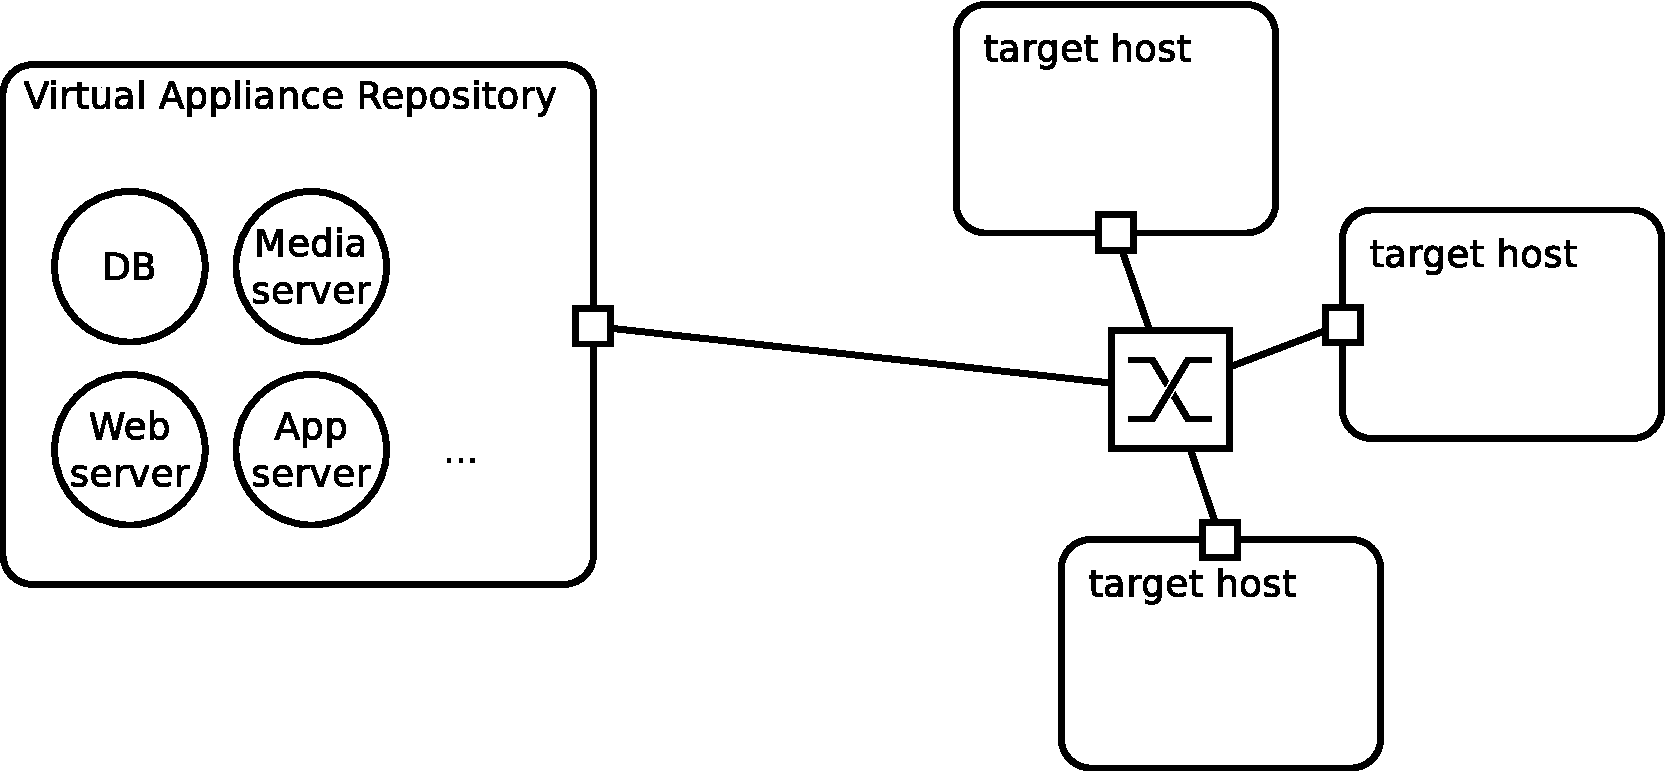
\includegraphics[width=.7\textwidth]{img/solaris/virtual-appliance-infra.pdf}
          \end{center}

          \caption{An example of infrastructure utilizing virtual appliances with appliance repository}
        \end{figure}


      \subsection{,,Network in a box'' concept}

        The ,,Network in a box'' term refers to virtual network topology hosted by a single machine (internal network
        virtualization). The topology consists of virtualized Layer 2 devices, virtual network machines (routers,
        firewalls, etc.) and virtual appliances providing specific high-level services. Moreover \gls{acr:qos} policies
        are applicable to enable network traffic differentiation. The solution allows to easily consolidate network
        topologies of arbitrary complexity and size.

        Thanks to the integration of multiple network-centric virtualization techniques, there are numerous advantages
        of the approach:

        \begin{itemize}

          \item the transmission is made more reliable and efficient with the use of virtualized data paths as physical
                links are not used and some packet processing stages can be omitted,

          \item policies driving the operation of virtual network machines can be easily changed with software-based
                implementation,

          \item services are deployed quickly and changed whenever needed as they are hosted on virtual appliances,

          \item fine-grained policies can be associated with specific classes of traffic to make the network
                \gls{acr:qos}-aware,

          \item high level of flexibility (hard to achieve in purely-physical environment) is provided, including
                topology reconfiguration (virtual appliance reattachment), \gls{acr:qos} policy management and control
                over physical resources consumption.
        
        \end{itemize}

        There can be multiple networks created inside single host system with guaranteed isolation. Also, the model can
        be extended to span multiple machines with topologies interconnected using \gls{acr:vlan}.

        There are existing virtualization solutions that support the model. The solutions differ in virtualization
        method used, \gls{acr:qos} support and efficiency. Most notable examples include Solaris OS (together with
        Containers and Crossbow technologies), VMWare and Xen.


    \section{Applications and benefits of virtual infrastructures}
    \label{sec:ctx:infra}

      Each IT company some day faces the challenge of partially utilized servers, low level of performance, low
      scalability and high complexity. Although there is no perfect solution for all those issues, virtual
      infrastructure is an approach gaining recently more and more supporters.  

      Things like lowering hardware, power and space requirements may be obtained thanks to accepting these approach.
      Beyond just system efficiency growth also effort necessary to put in configuring a system is smaller. 


      \subsection{Simulations and testing}

        Setting up networking environment when testing new protocols or topology operation itself can be hard or even
        impossible due to the costs. Even if successful, the topology is not flexible and adjustable --- these two
        crucial requirements for simulations and experimental studies are not met.

        Virtual infrastructures offer an alternative approach --- the environment to be tested can be easily created,
        often within a single physical machine, and used to perform the simulations. The parameters of the whole system
        can be adjusted whenever needed. Moreover, the approach does not require specialized hardware resources, thus it
        is cheaper. After necessary tests have been performed, the virtual model can be mapped directly to physical
        implementation, if necessary.

        The impact of virtualization on software development and testing process is also important. Software development
        teams can use fully virtualized environments --- reflecting the characteristics of actual ones --- to build,
        test and deploy software. The resulting flexible environment can be easily duplicated or restored to some
        specific state when needed.


        % Virtual infrastructure gives ability to provision new applications easily and quickly. As it is presented and
        % described in more detail in chapter \ref{chap:cs} creating any network structure consisting of any number of
        % virtual elements is easier than ever thanks to virtualized infrastructure. 


      \subsection{Server virtualization}
        
        There are multiple advantages of utilizing virtualization in server management. These benefits include, among
        others, reducing maintenance costs, flexibility and scalability.

        A number of logical servers can run inside single machine at the same time with network connectivity and
        resource sharing (e.g. read-only file system) enabled, if needed. Thanks to this consolidation, hardware
        spendings are significantly reduced and the centralized infrastructure is easier to administer. Moreover, the
        resources can be assigned dynamically, depending on the demand, allowing efficient hardware utilization
        \cite{server-consolidation}.

        Depending on virtualization type, the host machine can run either multiple instances of the same operating
        system (lightweight partitioning) or independent systems provided by different vendors (full virtualization).
        In both cases, the instances can be fully isolated to prevent interference between applications running inside.
        The flexibility makes virtualizing complex heterogneous environments easier.

        Replication and restoration on any target machine is simpler with virtualized servers. This property is
        particularly useful when designing and executing disaster recovery activities --- in case of system failure the
        whole infrastructures can be reprovisioned immediately, allowing business continuity for crucial services to
        remain intact \cite{vib}.

        Finally, legacy systems can also be integrated as a part of virtual infrastructure. Specific software and
        hardware requirements of these systems can be reconstructed in a virtualized environment to allow seamless
        migration and interoperation with other virtualized components. The approach allows to reduce substantial
        expenses associated with legacy systems maintenance that many \gls{acr:it} organizations bear \cite{boers}.


      \subsection{Infrastructure as a service}

        \gls{acr:iaas} refers to providing hardware (network, storage, computing resources) and software (operating
        system) as a service --- the service provider owns the underlying equipment and is responsible for housing,
        running and maintenance. The infrastructure can be highly personalized with respect to network topology,
        \gls{acr:qos} policies, computing power or provided software. The user is charged depending either on the
        contract signed or resource consumption (pay-per-cycle) \cite{iaas}.

        The on-demand infrastructure has to fulfil the requirements of flexibility and scalability. Thus, ability to use
        virtualized resources when providing \gls{acr:iaas} is crucial, both for customer and provider. The customer has
        access to isolated environment that --- as far as usage is considered --- is not different from a physical one
        and that can be expanded as needed, whereas the provider consolidates the services and makes efficient use of
        their hardware resources \cite{iaas}.

        % The \gls{acr:iaas} sometimes also called \gls{acr:haas} is one of three cloud computing models, the other two
        % are: \gls{acr:saas} and \gls{acr:paas}. This service is based on providing by the supplier whole scalable IT
        % infrastructure depending on user demand such as virtualized hardware. The service provider owns the equipment
        % and is responsible for housing, running and maintaining it.

        % At the beginning the \gls{acr:iaas} was just renting dedicated servers services from supplier. Nowadays thanks
        % to virtualization these are most often virtual machines. In the former case user paid for the concrete hardware
        % (box), now client typically pays on a per-use basis.


      \subsection{The role of virtualization in Service-oriented Architecture}

        \gls{acr:soa} is an architectural approach with main focus on building \gls{acr:it} systems as sets of loosely
        coupled services linked together and utilizing common communication infrastructure to interoperate. Given a
        business process, a service can be thought of as a repeatable task within the process. Services expose their
        interfaces, hiding implementation-, organization- or time-dependent details. It is important that the design of
        the \gls{acr:soa}-compliant system reflects the design of the business process \cite{soa-foundation}.

        Virtualization plays important role supporting the \gls{acr:soa}. The Infrastructure Services part of the
        logical model (depicted in figure \ref{fig:ctx:soa-logical}) uses virtualization extensively to provide secure,
        isolated, flexible and reliable execution environment to deploy and run services. Moreover, hardware usage can
        be optimized with single machine hosting multiple virtual environments \cite{soa-foundation}.

        \begin{figure}[h]
          \begin{center}
            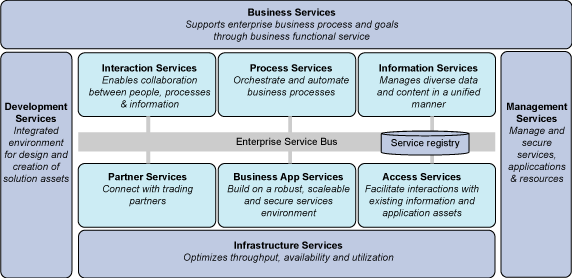
\includegraphics[scale=.5]{img/ctx/soa-logical.png}
          \end{center}

          % TODO przerysowac!

          \caption{Logical Service-oriented Architecture model}
          \label{fig:ctx:soa-logical}
        \end{figure}

        \gls{acr:s3} (figure \ref{fig:ctx:soa-stack}) is a high-level model depicting the functional and nonfunctional
        layers of an \gls{acr:soa} solution.  The \gls{acr:s3} shows the separation of concerns of the nine layers and
        imposes a border between service providers and consumers. In \gls{acr:s3}, virtual appliances are leveraged to
        provide on-demand applications building the Operational Systems layer \cite{soa-stack}.

        \begin{figure}[h]
          \begin{center}
            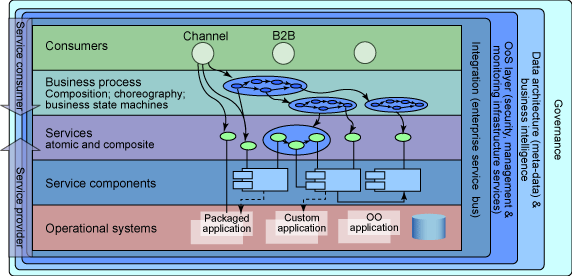
\includegraphics[scale=.5]{img/ctx/soa-stack.png}
          \end{center}

          % TODO przerysowac!

          \caption{Logical layers in the SOA Solution Stack}
          \label{fig:ctx:soa-stack}
        \end{figure}


    \section{QoS-aware networking}
    \label{sec:ctx:qos}

      % TODO  krotki przeglad QoS w roznych sieciach, nie tylko IP, ale tez ATM, Frame Relay, Token Ring (na podst.
      % wykl. Luke-a?)
      %
      % w szczegolach o QoS na IP

      \gls{acr:qos} is an issue in all types of networks such as \gls{acr:ip}, Token Ring, Frame Relay or even
      \gls{acr:atm}.  Each of them adapted specific approach towards this matter. \gls{acr:ip} network for instance is
      non-deterministic although there is a possiblity of packet classification using \gls{acr:cos} field. Token Ring on
      the other hand is deterministic and allows using priority to distinct traffic. Last but not least \gls{acr:atm}
      creates virtual path between sender and receiver and sets \gls{acr:qos} parameters. Despite the fact that all
      approaches are very interesting and meaningful this paper focuses mainly on the \gls{acr:ip} network and its
      approach to \gls{acr:qos}.

      % IntServ, DiffServ, inne

      Nowadays the \gls{acr:ietf} is working on two approaches beyond the basic best-effort service to provide more
      advanced handling of packets and providing requested level of bandwidth and delay which are:

      \begin{enumerate}
        \item integrated services --- reserves resources necessary to provide the service along path,
        \item differentiated services --- do not require resource reservation along path
      \end{enumerate}


      \subsection{DiffServ}

        Due to clear need for relatively simple and coarse methods of providing differentiated classes of service for
        Internet traffic, to support various types of applications, and specific business requirements. The
        differentiated service approach to providing quality of service in networks employs a small, well-defined set of
        building blocks from which a variety of aggregate behaviors may be built. \cite{qos}

        DiffServ works with traffic stream containing many complex microflows which among the same stream have:

        \begin{itemize}
          \item Same \gls{acr:qos} requirements,
          \item Traverses domain towards the same direction.
        \end{itemize}

        Microflow is a flow between applications and is identified mainly by:

        \begin{enumerate}
          \item Source and/or Destination Address,
          \item Transport protocol,
          \item Source and/or Destination Port.
        \end{enumerate}

        \begin{figure}[h]
          \begin{center}
            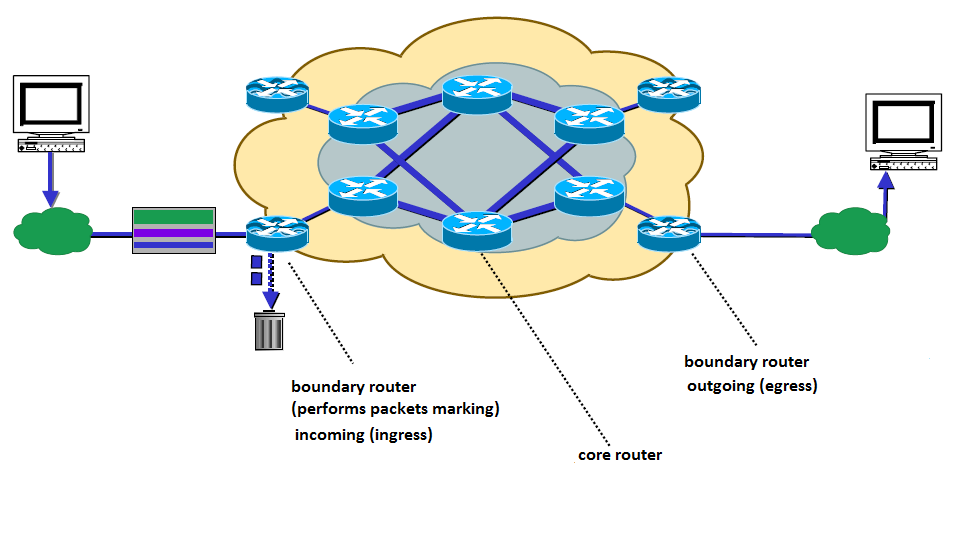
\includegraphics[width=.7\textwidth]{img/qos/diffserv.png}
          \end{center}

          % TODO przerysowac!

          \caption{DiffServ domain \cite{qos2}}
        \end{figure}

        DiffServ domain is a set of nodes with consistent \gls{acr:qos} policy (for example network managed by the same
        \gls{acr:isp} or intranet). Routers within domain are divided into two groups: boundary routers and core
        routers. Boundary router performs traffic classification, packet marking, traffic metering, traffic control
        (policing, shaping) where core routers pass packets according to \gls{acr:phb} and sometimes changes
        \gls{acr:dscp} labels. \cite{qos2}

        This architecture distinguishes two major components: packet marking using the IPv4 ToS byte or TC in IPv6 and
        \gls{acr:phb}.

        \medskip

        Redefined ToS field now uses 6 bits for packet classification and is called \gls{acr:dscp}. \gls{acr:phb}
        defines how packet should be treated due to its priority. Accepted policy should be consistent within all
        domain.


      \subsection{IntServ}

        Integrated services beyond the basic best-effort service defined in two \gls{acr:rfc} documents provide two
        levels of service for \gls{acr:ip} which are called Controlled-Load Service and Guaranteed Service. Both require
        information about the traffic to be generated. 

        Guaranteed Service type should be used in applications with real time demands as it provides guaranteed
        bandwidth and delay, whereas Controlled-Load Service does not give full guarantee and should be used with
        application less sensitive for packets loss or delay.

        IntServ requires resource reservation for certain flows or aggregated data streams. The reservation operation is
        available thanks to \gls{acr:rsvp}. Due to this reservation session initialization lasts much longer than in
        DiffServ \cite{qos2}.

        \begin{table}[ht]
          \centering
          \begin{tabular}{|c|c|}
            \hline
            IntServ         & DiffServ \\
            \hline \hline
            Stateful        & Stateless \\
            \hline
            Not scalable    & Scalable \\
            \hline
            Stream oriented & Processing single packets \\
            \hline
          \end{tabular}

          \caption{Comparison of DiffServ and IntServ}
        \end{table}


    \section*{Summary}

      The chapter presented general information about resource virtualization together with examples of the approaches and
      implementations being in common use in the domain. The importance of network virtualization was emphasized and
      multiple aspects of network topology virtualization were covered --- internal and external virtualization,
      partitioning and creating logical software-based networking devices. Also, one of the core concepts of virtual
      infrastructure management --- virtual appliances --- was introduced and its advantages were listed.

      The selected applications of virtual network infrastructures confirm the importance of virtualization techniques
      in modern systems management, service provisioning, sophisticated software development and testing. The
      flexibility and scalability that virtualization offers compared to hardware solutions makes it a natural choice when
      building enterprise class architectural frameworks, like \gls{acr:soa}.

      Despite the fact that the concept of virtualization is not new, it is still one of the most discussed and
      investigated fields in the area of computer science. Innovative ideas and solutions emerging incessantly and the
      impact they have on the way computing is perceived is what makes virtualization interesting both as a tool and
      a subject of research.


  \chapter{Requirements analysis}
  \label{chap:req}

    The chapter presents initial phase of the system development --- requirements analysis. The established goal is to
    design architecture and system implementing it that supports creation of any requested, fully isolated virtual
    network topology with ability to monitor its operation. This objective implicates the necessity of creating
    requirements specification in order to avoid ambiguities and skipping essential services.

    Section \ref{sec:req:spec} introduces objects and processes discussed throughout the thesis. Formal definition is
    provided for each term. Also, high-level view of the domain is depicted to give better understanding of the subject.

    Section \ref{sec:req:func} lists functional requirements the architecture has to fulfill. The requirements are
    grouped to reflect main coarse-grained processes.
    
    Section \ref{sec:req:nonfunc} describes two classes of identified non-functional requirements. Run-time qualities
    (related to user goals) and development-time qualities are discussed.

    Finally, execution environment requirements are gathered in section \ref{sec:req:env}. These describe underlying
    environment characteristics such as isolation and preservation of broadcast domain.


    \section{Domain specification}
    \label{sec:req:spec}

      To provide common vocabulary, make the requirements specification clearer and avoid ambiguities, definitions of
      crucial domain elements and processes are provided in table \ref{tab:req:def}. These definitions are referred to
      throughout the subsequent discussion.

      \begin{table}[H]
        \centering

        \begin{tabularx}{\textwidth}{|l|X|}
          \hline
          \multicolumn{1}{|c|}{Term}     & \multicolumn{1}{c|}{Definition}                                            \\
          \hline \hline
          Virtual topology               & Computer network topology built using virtualized links, \gls{acr:nic}s,
                                           switches, appliances, etc. together with \gls{acr:qos} policies defined    \\
          \hline
          Virtual topology model         & Abstract, implementation-independent description of a virtual topology     \\
          \hline
          Flow                           & A class of network traffic                                                 \\
          \hline
          Host machine                   & Physical or virtual machine with an operating system capable of hosting
                                           a virtual topology                                                         \\
          \hline
          Underlying network environment & A group of host machines connected with \gls{acr:lan}                      \\
          \hline
          Instantiation                  & The process of transforming virtual topology model to actual topology
                                           deployed on host machines                                                  \\
          \hline
          Discovery                      & Automatic process of examining existing virtual topology and recreating
                                           virtual topology model                                                     \\
          \hline
          Monitoring                     & Accessing historical information about topology operation (e.g. bandwidth
                                           consumption)                                                               \\
          \hline
        \end{tabularx}
        
        \caption{Important problem domain terms and their definitions}
        \label{tab:req:def}
      \end{table}

      Figure \ref{fig:req:overview} presents an overview interoperation between objects and processes defined. The
      monitoring functionality provided is required to operate on the virtual topology model rather that the topology
      itself.

      \begin{figure}[H]
        \centering
        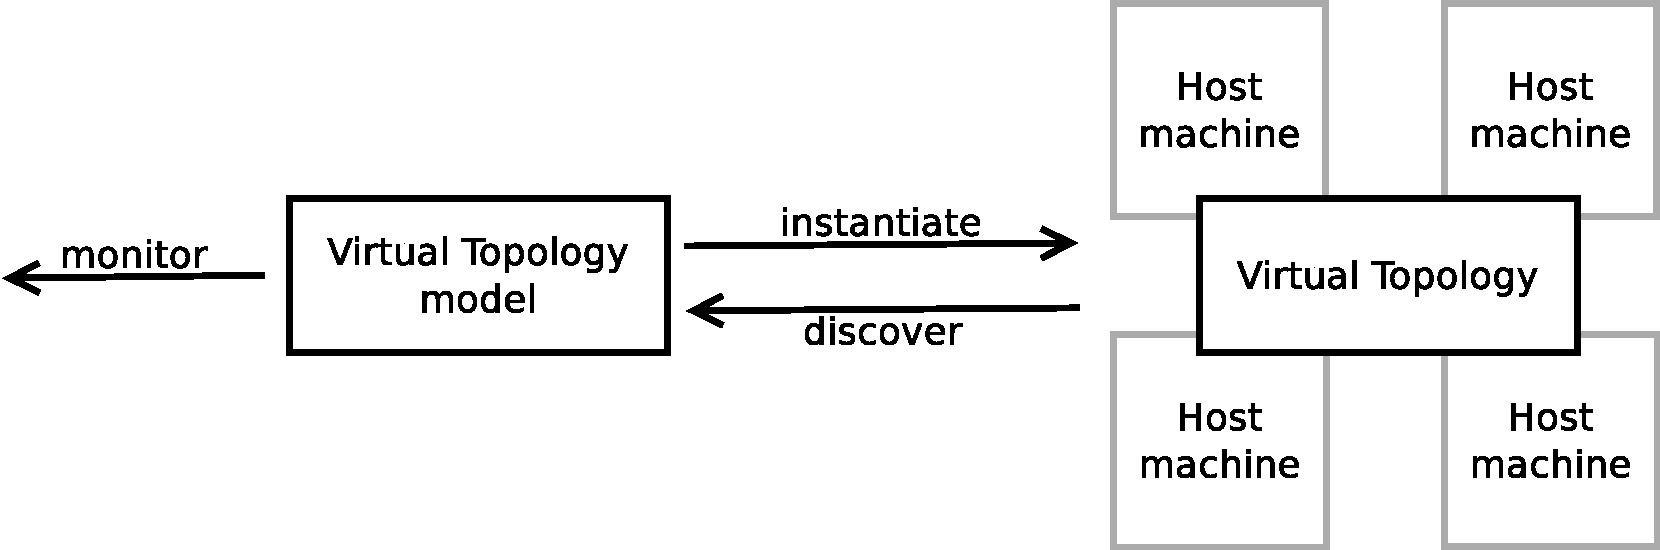
\includegraphics[width=.7\textwidth]{img/req/overview.pdf}

        \caption{Important high-level objects and processes}
        \label{fig:req:overview}
      \end{figure}


    \section{Functional requirements}
    \label{sec:req:func}

      All services of the system are divided into four groups --- topology design, instantiation, discovery and
      monitoring. This division reflects the main processes identified when working with virtual infrastructures.
      Detailed description of each group follows.

      \todo[inline]{diagram: review}

      \begin{figure}[H]
          \centering

          \begin{tikzpicture}[rotate=90]
            \begin{umlsystem}[x=6, y=7, fill=red!10]{The CM4J core system}
              \umlusecase[x=-4, y=4]{creation of network structure}
              \umlusecase[x=-2, y=5.5, fill=green!20]{CRUD operations for network virtual elements}
              \umlusecase[x=-6, y=1.5, fill=green!20]{CRUD operations for virtual resources}
              \umlusecase[x=-6, y=8.5, fill=green!20]{applying QoS limits}
              \umlusecase[x=0.5, y=5]{network virtual element's bandwidth monitoring}
              \umlusecase[x=-1, y=0]{network statistics monitoring}
              \umlusecase[x=-10, y=4]{network project structure discovery}
              \umlusecase[x=-7, y=1, fill=green!20]{virtual resource discovery}
              \umlusecase[x=-12, y=1, fill=green!20]{virtual elements discovery}
              \umlusecase[x=-8, y=7, fill=green!20]{assigned QoS limits discovery}
            \end{umlsystem}

            \umlactor{user}[y=-6]

            \umlassoc{user}{usecase-1}
            \umlassoc{user}{usecase-2}
            \umlassoc{user}{usecase-3}
            \umlassoc{user}{usecase-5}
            \umlassoc{user}{usecase-6}
            \umlassoc{user}{usecase-7}
            \umlassoc{user}{usecase-8}
            \umlassoc{user}{usecase-9}

            \umlinclude[name=incl]{usecase-8}{usecase-7}
            \umlinclude[name=incl]{usecase-9}{usecase-7}
            \umlinclude[name=incl]{usecase-10}{usecase-7}
            \umlinclude[name=incl]{usecase-2}{usecase-1}
            \umlinclude[name=incl]{usecase-3}{usecase-1}
            \umlinclude[name=incl]{usecase-4}{usecase-1}
          \end{tikzpicture}

          \caption{Functional requirements use-case diagram.}
        \end{figure}


      \subsection{Virtual topology design and adjustment}

        The process of network design and adjustment is among the most important considerations. It is the main
        way the user is able to define and change virtual topologies. Virtual topology model is used to manipulate
        virtual topologies --- no underlying details are exposed to the user or other high-level components.

        The user designing a virtual topology from scratch or modifying an existing topology should be able to:

        \begin{itemize}
          \item create, modify, delete components of the topology (interfaces, switches, routers),
          \item access appliance repository and select appliances that should be a part of the topology,
          \item assign interfaces to appliances and routers,
          \item enable and alter routing tables to enable communication between different \gls{acr:ip} subnetworks,
          \item manage \gls{acr:qos} policies (assign priorities and limit bandwidth of network traffic flows),
          \item assign parts of the model to available host machines.
        \end{itemize}


      \subsection{Instantiation}
      \label{sec:req:func:inst}

        The system should support virtual topology instantiation --- for any correct virtual topology model it should be
        possible to create corresponding virtual components that implement the model. Instantiation process should:

        \begin{itemize}
          \item be automatic --- no extra intervention is required from user to deploy the model,
          \item be atomic --- either all the elements of topology are instantiated successfully or the process is rolled
                back,
          \item support deployment of multiple topologies on a single host machine,
          \item support topologies spanning multiple host machines,
          \item provide optional automatic topology assignment in accordance with predefined rules.
        \end{itemize}


      \subsection{Discovery}
      \label{sec:req:func:disc}

        Instantiated virtual topologies should be discoverable automatically. The discovery process is an inverse of
        instantiation. The required functionalities are:

        \begin{itemize}
          \item distinguishing multiple topologies deployed on a single host machine and returning separate models for
                them,
          \item support for topologies spanning multiple host machines.
        \end{itemize}


      \subsection{Monitoring}
      \label{sec:req:func:acc}

        When instantiated, a topology is subject to monitoring. The user still uses the model to query particular
        statistics --- implementation details remain hidden. Monitoring functionality should:

        \begin{itemize}
          \item allow to access interfaces, switches and routers and gather statistical data,
          \item provide multiple levels of granularity (bit, byte, packet),
          \item store the data so that it can be read and analyzed in the future,
          \item present statistics in a clean and readable way.
        \end{itemize}


    \section{Non-functional requirements}
    \label{sec:req:nonfunc}

      Two main groups of non-functional requirements (qualities) of a system can be distinguished --- there are run-time
      qualities (related to user goals) and development-time qualities (related to development organization goals)
      \cite{nonfunctional}.

      Main run-time qualities the system should meet are:

      \begin{itemize}
        \item usability --- \gls{acr:gui} should be intuitive and allow to perform operations effectively,
        \item configurability --- configurable properties should be easy to set,
        \item adaptable --- ability to adapt to changing conditions (unstable underlying environment),
        \item fault tolerance --- system should be resistant to errors (incorrect input should not break the system's
                                  operation).
      \end{itemize}

      Development-time requirements to fulfill are:

      \begin{itemize}
        \item independent and reusable object model --- the model should be general, independent of system-specific
                                                        details,
        \item evolvability --- support for new functionalities or adjustment to new technologies should be easy,
        \item extensibility --- ability to add new, earlier unspecified functionalities; open/closed principle should be
                                applied while designing the system,
        \item composability --- system should be created in form of composable, highly-cohesive components,
        \item reusability --- ability to (re)use and embed in other systems; \gls{acr:api} version dependent on required
                              level of abstraction.
      \end{itemize}


    \section{Underlying environment characteristics}
    \label{sec:req:env}

      Underlying environment should be a composition of fully independent nodes. However, there are requirements that
      must be fulfilled by each node to allow the system to work properly.

      The chosen operating system must provide mechanisms for isolation among virtualized elements, so that one's
      processor or memory usage does not affect corresponding resources performing other operations. Also, there cannot
      be any interference between different topologies hosted on the same machine.

      The broadcast domain has to be preserved, too --- i.e. there has to be isolation starting from the link layer of
      the \gls{acr:osi} model. Every instantiated infrastructure should preserve its broadcast domain in order to
      achieve network traffic isolation between different projects to fulfill the thesis statement. To achieve that,
      separate \gls{acr:vlan} per project should be created or any other equivalent approach should be adopted.


    \section*{Summary}

      This chapter provided thorough analysis of system requirements. After the vocabulary of crucial terms have been
      established, all the requirements (both functional and non-functional) which the implemented \gls{acr:cm4j} is
      expected to fulfill were described. Also, expectations towards underlying environment were presented. In order to
      meet all the aforementioned constraints the system has to be implemented under OS supporting network and resource
      virtualization with ability to isolate infrastructure operation and restrict broadcast domains.


  \chapter{Solaris 10, Solaris 11 and OpenSolaris}
  \label{chap:sol}
  
    %TODO change chapter title !!! // Solaris OS as a resource virtualization environment
    % TODO  actually, Solaris 10, Solaris 11 and OpenSolaris are described here!

    The chapter provides an overview of Oracle Solaris operating system and evaluates it as a platform for resource
    virtualization. The chapter describes Solaris 11 Express release of the system, as it is the first release (together
    with OpenSolaris) with Crossbow technology integrated. Special emphasis is put on the networking-related aspects of
    virtualization. Thus, the Solaris Crossbow technology is described in detail.

    Section \ref{sec:sol:general} contains introductory information about the system. A short historical note is
    presented and general description follows. Main components of the system are introduced and described.
    
    Each of the remaining sections describe in more detail these parts of the operating system that are extensively used
    by the implemented system. Section \ref{sec:sol:containers} investigates the Solaris Zones technology. After
    defining the concept of zones, zone lifecycle model is presented, the achieved level of process isolation is
    described and discussion of Zones advantages in comparison to non-virtualized environments follows.

    Section \ref{sec:sol:xbow} introduces Solaris Crossbow - lightweight network virtualization environment. The section
    starts with general description of the technology. Next, components crucial to efficiency improvement are presented
    in detail. Etherstubs, \gls{acr:vnic}s and flows are described. These are building blocks used to create virtualized
    network elements and apply \gls{acr:qos} policies. The section ends with the comparison between Crossbow and
    DiffServ and a method of integration of these two solutions is presented.

    Section \ref{sec:sol:res} provides an overview of resource control methods offered by the Solaris OS. The types of
    resource management mechanisms (constraints, partitioning and scheduling) are identified and defined. Resource
    control hierarchy used by the system is depicted and explained. Also, the accounting facility is described. The
    types of resources extended accounting can work with are enumerated and examples of data that can be gathered are
    listed.


    \section{General information}
    \label{sec:sol:general}

      Oracle Solaris is a \textit{multiuser, multitasking, multithreading UNIX-like operating system} \cite{reference}.
      Since its release in 1992 (as Sun Solaris 1), the system became one of the most popular environments supporting
      enterprise software. Nowadays, big corporations and companies as well as individual developers use it to do their
      business and deliver reliable and scalable services.

      The Solaris OS provides unique set of tools that support virtualization of practically all types of resources at
      various levels. There is \gls{acr:ldom} technology for full virtualization and lightweight Zones, when all that is
      needed is the isolation of processes. Logical domains can be connected with complex virtual networks that are
      created with virtual switches (vsw) and virtual network devices (vnet) \cite{ldomag} and Crossbow can be used to
      enable lightweight and efficient networking for zones, exploiting capabilities of underlying hardware layer
      (network interface cards with virtualization level 1, 2 or 3 \cite{santos}).

      Resource utilization can be managed with integrated administration tools. Resource access policies can be created
      with high level of granularity (per-process resource control) as well as in more general way (limiting resource
      access for \gls{acr:ldom}s). Resource consumption can be subject of monitoring and accounting. With extended
      accounting subsystem enabled, it is possible to capture detailed accounting data even for single processes.
      Gathered data include CPU usage, number of bytes received or transmitted per DiffServ or Crossbow flow and more.

      As far as multiple physical machines are considered, there is also support for \gls{acr:vlan}.  Thanks to
      \gls{acr:vlan} tagging support, it is possible to build systems that guarantee the quality of service from the
      lowest levels up, even for services belonging to different systems and consolidated within single physical
      machine.

      \begin{figure}[H]
        \begin{center}
          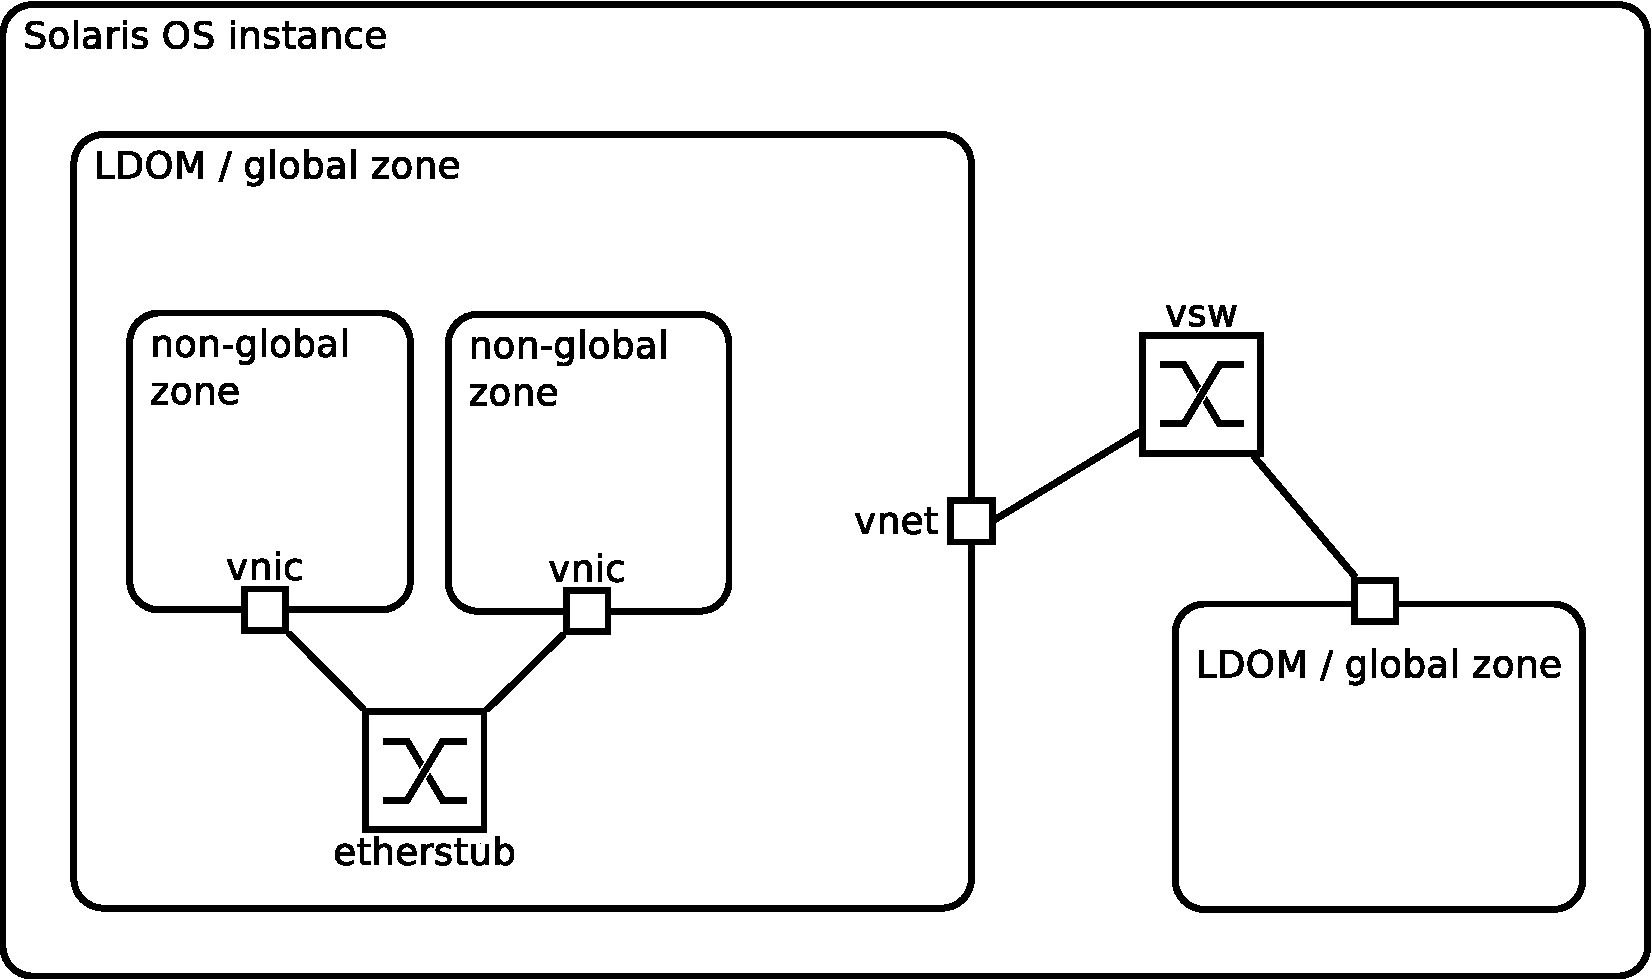
\includegraphics[width=.7\textwidth]{img/solaris/full-featured.pdf}
        \end{center}

        \caption{The variety of resources that can be virtualized with Solaris OS}
      \end{figure}

      As it can be seen, the Solaris operating system is accompanied by vast variety of virtualization-supporting
      subsystems. This multiplicity and flexibility makes it a promising platform for service provisioning and building
      even more abstract architectures on top of it. The following sections describe selected aspects of the system in
      more detail.


    \section{OS-level virtualization with Solaris Containers}
    \label{sec:sol:containers}

      The concept of lightweight (OS-level) virtualization is supported by most modern operating systems. The solutions
      are either integrated into the system's kernel and accessible as soon as it is installed (Solaris Containers, AIX
      Workload partitions, BSD jails \cite{kamp}) or are provided by third-party manufacturers as kernel patches and
      utility software (OpenVZ and \gls{acr:lxc} for Linux OS). Because of awareness of other system components and
      integration with them, it can be expected that Zones have more potential than other virtualization methods.


      \subsection{General information}
      \label{sub:}

        Zones technology was introduced as of Solaris OS 10. It provides a way of partitioning system resources and
        allows for isolated and secure application execution environment \cite{sag}. Solaris Zones, together with
        resource management functionality, constitute the Solaris Container environment.

        There are two types of zones: global and non-global. Global zone is the default one and is used to execute
        applications as well as to administer the system. Non-global zones can be created from within the global zone
        only. A single operating system instance with one global zone can host as many as 8192 non-global zones
        \cite{sag}.

        Zones can be assigned system resources such as CPU capacity, the amount of random-access memory or even maximum
        number of lightweight processes that can be running simultaneously. Also, network isolation is supported at two
        levels: basic, at the \gls{acr:ip} layer, and network isolation and advanced virtualization with fine grained
        quality of service control using the Crossbow technology.

        Each zone can run a different set of applications, with optional translation of system calls (Branded Zones
        Technology) thus emulating different operating environments \cite{sag}. The user is able to create a branded
        zone with translation of Linux system calls and run Linux-specific applications without code recompilation.

        \begin{figure}[H]
          \begin{center}
            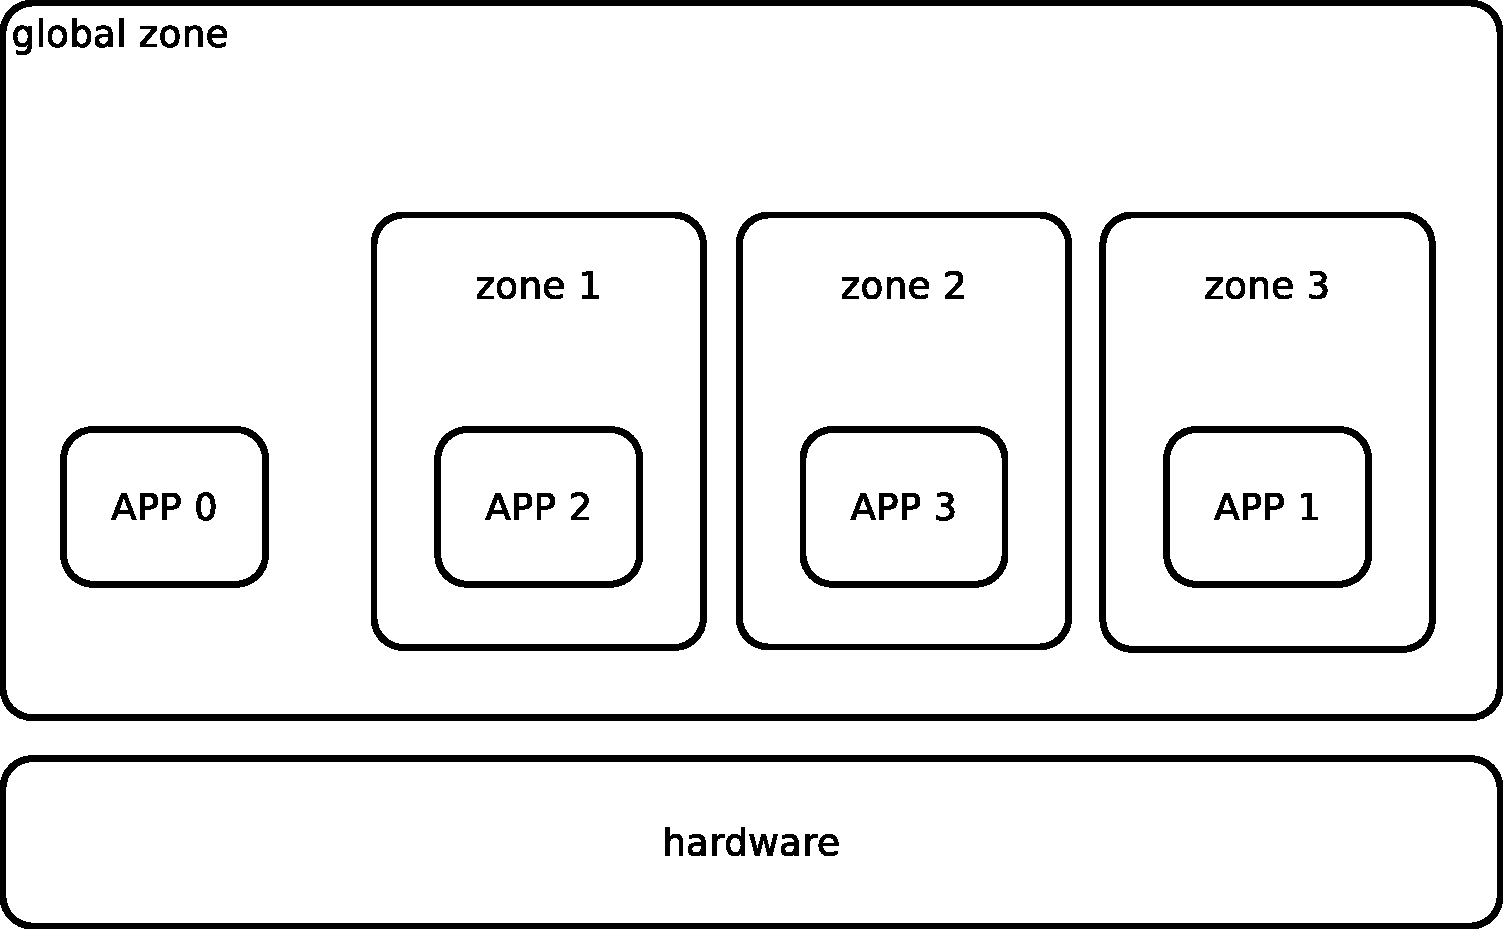
\includegraphics[width=0.7\textwidth]{img/solaris/zones-high-level.pdf}
          \end{center}

          \caption{Solaris Zones high-level view}
        \end{figure}


      \subsection{Zone lifecycle}
      \label{sub:}

        A model was created to describe the states in which each zone must exist and its possible transitions. A
        non-global zone can be in one of six states: \textit{configured}, \textit{incomplete}, \textit{installed},
        \textit{ready}, \textit{running}, \textit{shutting down or down} \cite{sag}. Figure \ref{fig:sol:lifecycle}
        depicts the model.

        \begin{figure}[H]
          \begin{center}
            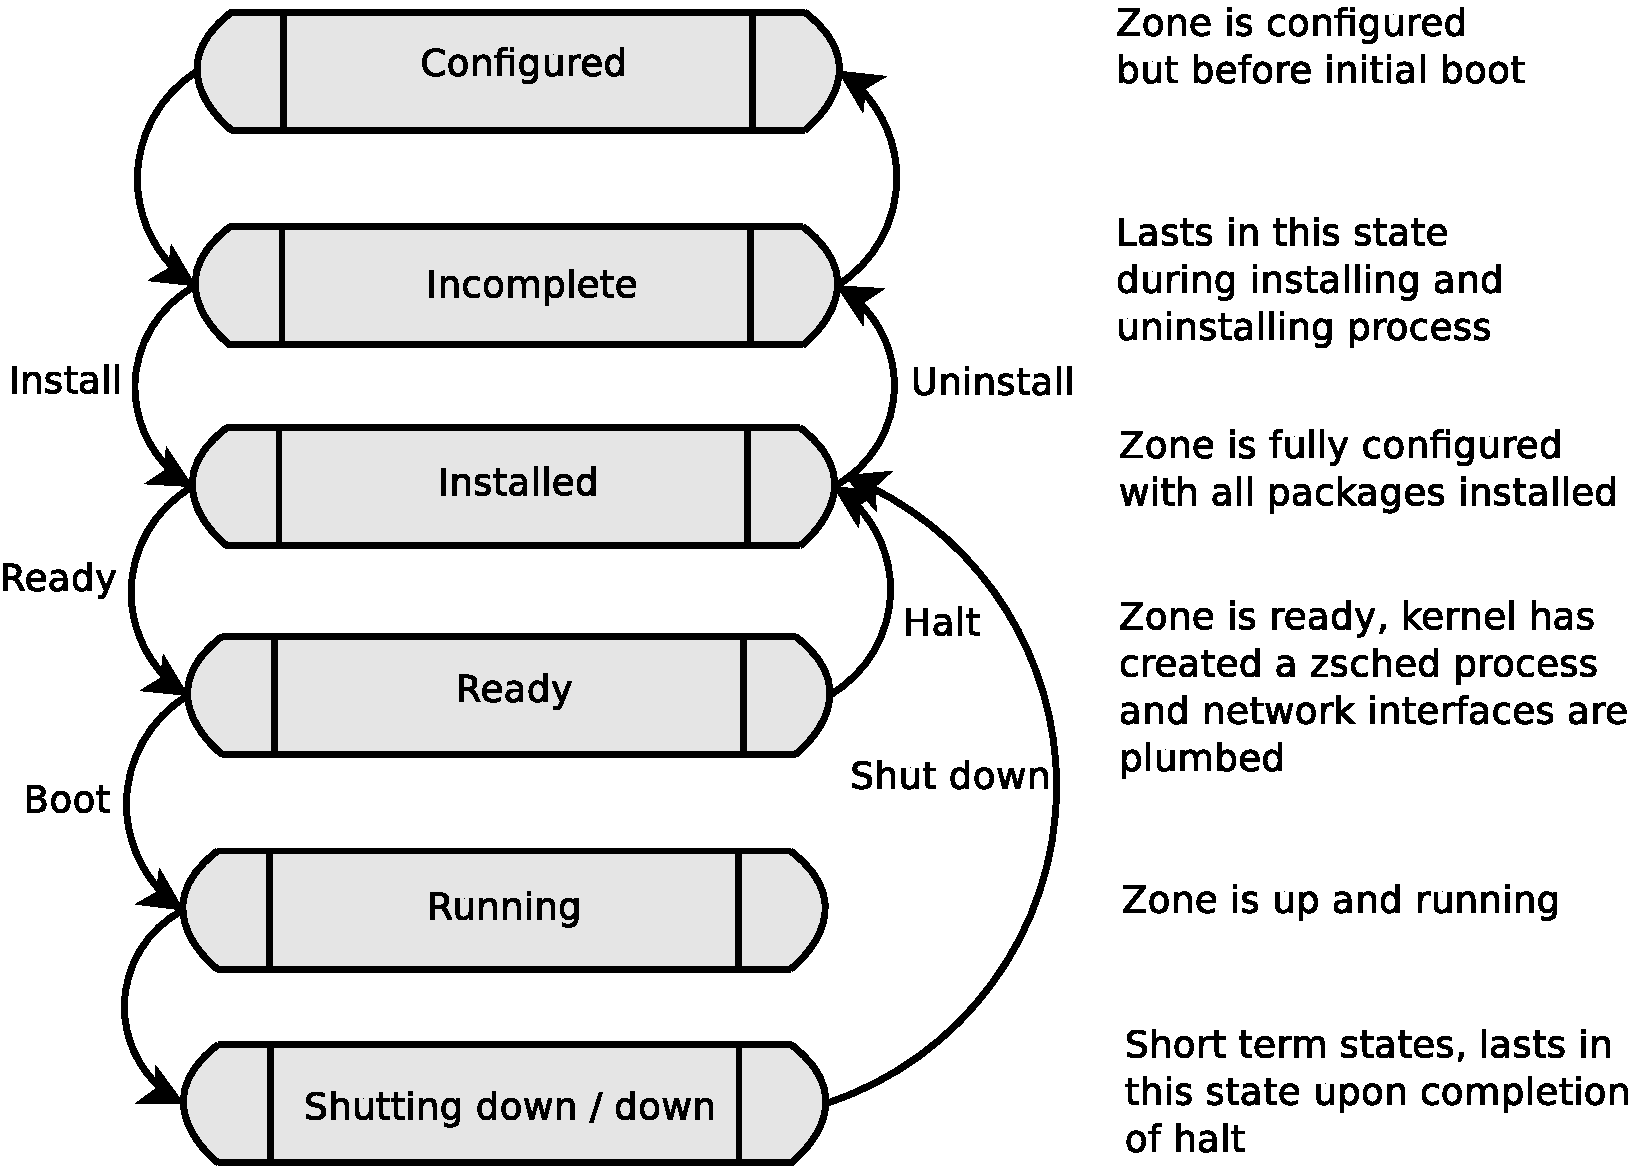
\includegraphics[width=0.7\textwidth]{img/solaris/zone_states.pdf}
          \end{center}

          \caption{Zone states and possible transitions}
          \label{fig:sol:lifecycle}
        \end{figure}


      \subsection{Isolation of processes}
      \label{sub:}

        The Containers environment offers a high level of application security and isolation. This is accomplished by
        imposing software bounds on the resource usage and introduction of additional abstraction layer over hardware.

        Every process and its children are bound to concrete zone and the assignment cannot be changed. Moreover, it is
        impossible for processes in distinct zones to monitor each other operation. They are not visible to each other
        and no interprocess communication can take place, except for network-based one, if enabled by the administrator.

        Because of the isolation, an application failure possibly affects only the processes in the containing zone.
        Assuming no interaction between processes in separate zones, the rest of the system remains intact and can
        operate normally.
        
        % TODO easier recovery, independent container management
      

      \subsection{Advantages of Containers technology when compared to non-virtualized environments}
      \label{sub:}

        The architecture of Solaris Containers makes it a competitive solution as far as systems administration and
        operation efficiency is concerned. The technology, imposing negligible overhead \cite{price}, allows to perform
        tasks that would be impossible or very hard to accomplish if traditional setup is used. Examples of such tasks
        include dynamic resource assignment, instantaneous cloning and migration of systems between physical nodes.

        The technology allows for running a number of isolated instances of operating system sharing CPU time, physical
        network bandwidth, filesystem contents and binary code. Sharing of these resources can greatly improve overall
        system efficiency and reduce the amount of occupied memory. The speed of network communication between different
        zones can also be improved thanks to ,,short-circuited'' traffic (ie. omitting the layers below \gls{acr:ip} in
        the \gls{acr:osi} stack). The instances are able to execute applications with minimum overhead introduced mainly
        due to accessing commands and libraries through the lofs (loopback filesystem) \cite{price,fsag}.

        When using file system that supports snapshots (as, for example, ZFS), zones can be serialized (a snapshot of
        the file system can be taken) and sent over the network connection or other means of data transfer to another
        machine. There, the zone can be restored and operate as a part of the host system.

        Another important aspect of building the infrastructure with containers is resource control. The Solaris system
        makes it possible to define resource controls (rctls) at various levels, also on per-zone basis. CPU shares,
        maximum number of lightweight processes and maximum swap size are examples of resource control properties that
        can be set for a zone. This can be further extended by providing fine-grained properties at project, task and
        process levels \cite{sag}. The resource control process is dynamic - assignments can be changed as the system is
        running, without interrupting the container's normal operation. This can be of extreme importance as far as
        high-availability systems are considered.

        Containers facilitate service consolidation - all components of a system can be executed in a single machine
        with network-based communication handled entirely by the host operating system, thus eliminating the need for
        additional networking hardware and its management. The consolidated infrastructure becomes more flexible as the
        majority of administration tasks can be performed by issuing a series of terminal commands. All these factors
        make total cost of ownership lower \cite{price}.

        \begin{figure}[H]
          \begin{center}
            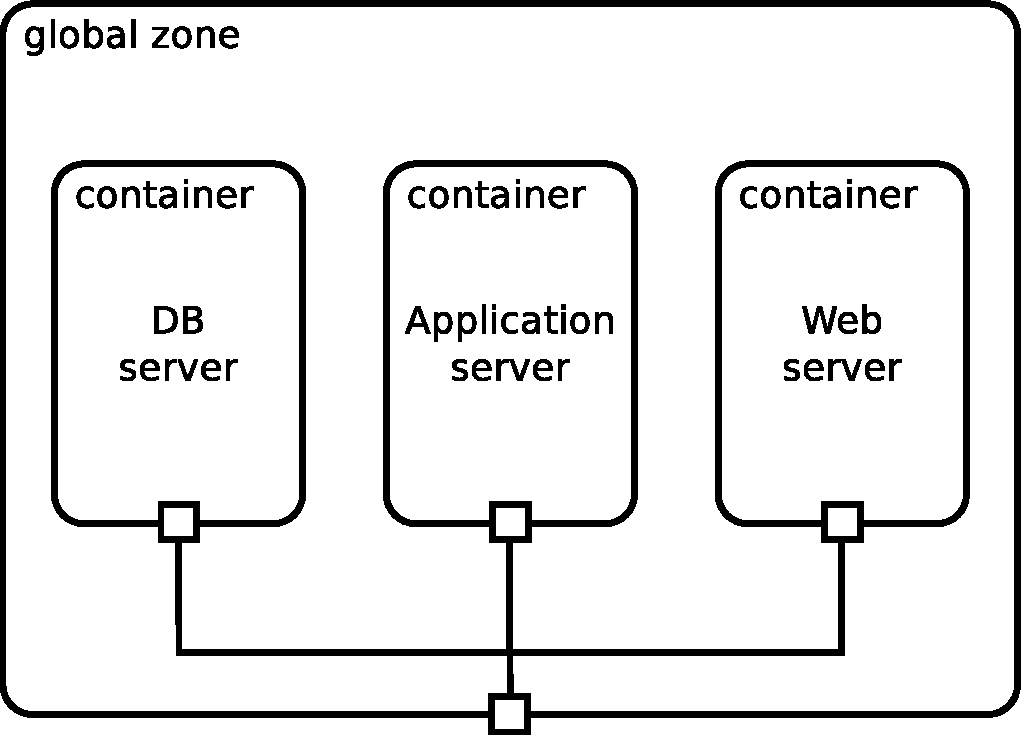
\includegraphics[width=.6\textwidth]{img/solaris/consolidation.pdf}
          \end{center}

          \caption{Service consolidation within a Solaris OS instance with internal network connectivity}
        \end{figure}


    \section{Crossbow - network virtualization technology}
    \label{sec:sol:xbow}

      % TODO when introduced? +citation

      It is generally acknowledged that Crossbow was invented in China in 341 B.C but it was in middle ages when it
      earned its recognition. Very easy in use and simultaneously very effective. The Solaris Crossbow mechanism for
      \gls{acr:qos} are just like real crossbows, very efficient in comparison to other existing \gls{acr:qos}
      mechanisms and this similarity indicates the project name origin.


      \subsection{Crossbow architecture}

        One of the most important conditions in terms of network virtualization is that network traffic should be
        insulated between virtual machines. This kind of isolation can be achieved by having a dedicated physical
        \gls{acr:nic}, network cable and port from the switch to the virtual machine itself. Moreover, switch must also
        ensure sustainability on every port. Otherwise, virtual machines will definitely interfere with each other
        \cite{crossbow}.
        
        In a particular case when a physical \gls{acr:nic} has to be shared between virtual machines the most promising
        solution is to virtualize \gls{acr:nic} hardware and the second layer of the \gls{acr:osi} stack where sharing
        is fair and interference will be avoided. These approach was adapted in the Crossbow architecture in the Solaris
        OS \cite{crossbow}.
        
        Traffic separation is achieved with fundamental blocks (\gls{acr:vnic}) of new architecture created by
        partitioning physical \gls{acr:nic}. A \gls{acr:vnic} can be created over \gls{acr:nic} or Etherstub and be
        dynamically controlled by the bandwidth and CPU resources assigned to it \cite{crossbow,network_virtualization}.
        New architecture after introducing new networking features combined with existing features like Solaris
        Containers, resource control can be presented as following:

        \begin{figure}[H]
          \begin{center}
            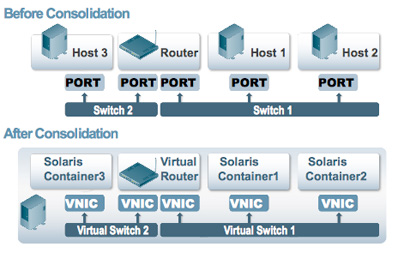
\includegraphics[width=.7\textwidth]{img/crossbow.jpg}
          \end{center}

          % TODO przerysowac!

          \caption{The Solaris Crossbow network virtualization enhancement, source: http://www.net-security.org/images/articles/crossbow.jpg}
        \end{figure}

        The crossbow architecture has introduced fully parallel network stack structure. Each stack could be seen as an
        independent lane (without any shared locks, queues, and CPUs) therefore network isolation is guaranteed. Key
        concept is hardware classification performed by the \gls{acr:nic} over which \gls{acr:vnic} was created. Each
        lane has a dedicated buffer for Transmit (Tx) and Receive (Rx) ring. In case when load exceeds assigned limit
        packets must be dropped as it is wiser to drop them than to expend OS CPU resources \cite{crossbow}.

        \begin{figure}[H]
          \begin{center}
            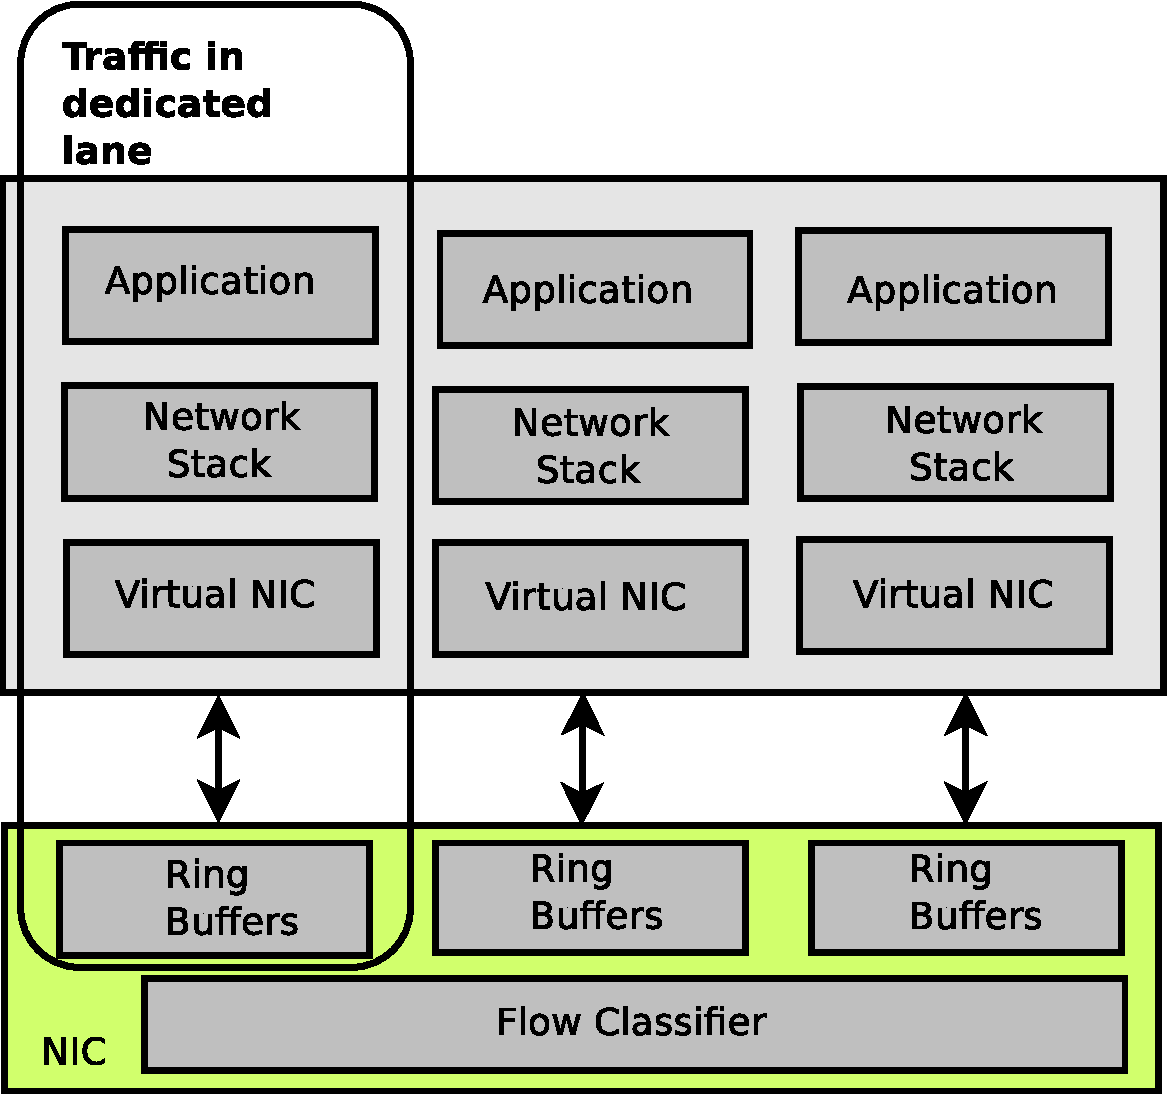
\includegraphics[width=0.5\textwidth]{img/crossbow-traffic-dedicated-line.pdf}
          \end{center}

          \caption{Dedicated lanes in the Crossbow architecture}
        \end{figure}

		
      \subsection{Virtualization lanes}

        Virtualization lane is the most key component in the Crossbow architecture. Each lane consists of some dedicated
        hardware and software that might be used to handle specific type of traffic. It usually would be composed of: 

        \begin{enumerate}
          \item \gls{acr:nic} resources (receive and transmit rings, interrupts, MAC address slots),
          \item Driver resources (DMA bindings),
          \item MAC layer resources (data structures, execution threads, locks).
        \end{enumerate}
        
        A virtualization lane can be one of two types, hardware-based or software-based.

        
        \subsubsection{Hardware-based virtualization lanes}
        
          This type requires ability to partitioning resources from \gls{acr:nic}. The minimum requirement is that a
          hardware-based lane should must have a dedicated receive ring. Other resources such as transmit lane can be
          exclusive or shared between lanes. Each virtual machine could have one or more lanes assigned and the incoming
          packets would be distributed among them based on even scheduling unless some administrative polices where
          created, such as priority or bandwidth limit \cite{crossbow}.		

        
        \subsubsection{Software-based virtualization lanes}
        
          In case when \gls{acr:nic} runs out of hardware-based virtualization lane, receive and transmit rings may be
          shared by multiple \gls{acr:vnic}s. The number of software-based virtualization lanes also often called
          softrings is unlimited. The main disadvantage of software-based lanes is the lack of fairness and isolation
          which in fact is provided in hardware-based lanes. The received and sent rings may work also in mix mode,
          whereas some of the rings may be assigned to software and some may be assigned to hardware based lanes
          \cite{crossbow}.	
			
      \subsection{Dynamic polling}	
        
        The Crossbow architecture proposed two types of working modes. Currently used mode is determined by traffic and
        load. Under low load, where the rate of arriving packets is lower than time of packet processing, a lane works in
        the interrupt mode which means that receive ring generates an interrupt when new packet arrives. However, when
        the backlog grows, the line switches to dynamic polling mode in which a kernel thread goes down to the receive
        ring in the \gls{acr:nic} hardware to extract all outstanding packets in a single chain. Key aspect is that every
        virtualization lane works independently and transparently from each other. Usually only three threads are used
        per lane \cite{crossbow}:
        
        \begin{enumerate}
          \item Poll thread which goes to the \gls{acr:nic} hardware to get all packet chain,
          \item Worker thread which is responsible for protocol processing (\gls{acr:ip} and above) or delivers packets
                to virtual machine. Thread performs also any additional transmit work which is a natural requirement
                some concrete protocol, such as processing TCP packets that require sending ACK packets,
          \item Transmit thread that is activated when if packets are being sent after transmit side flow control relief
                discharge, or after retrieving transmit descriptor. Application or virtual 
                machine can transmit any packets without performing queuing because of flow control or context switching.
        \end{enumerate}


      \subsection{Virtual switching}
        
        Virtual switches are always created implicitly when the first \gls{acr:vnic} is defined under existing
        \gls{acr:nic} and could never be accessed directly nor be visible by any user (even administrator)
        \cite{crossbow2}. 
        
        \begin{figure}[H]
          \centering
          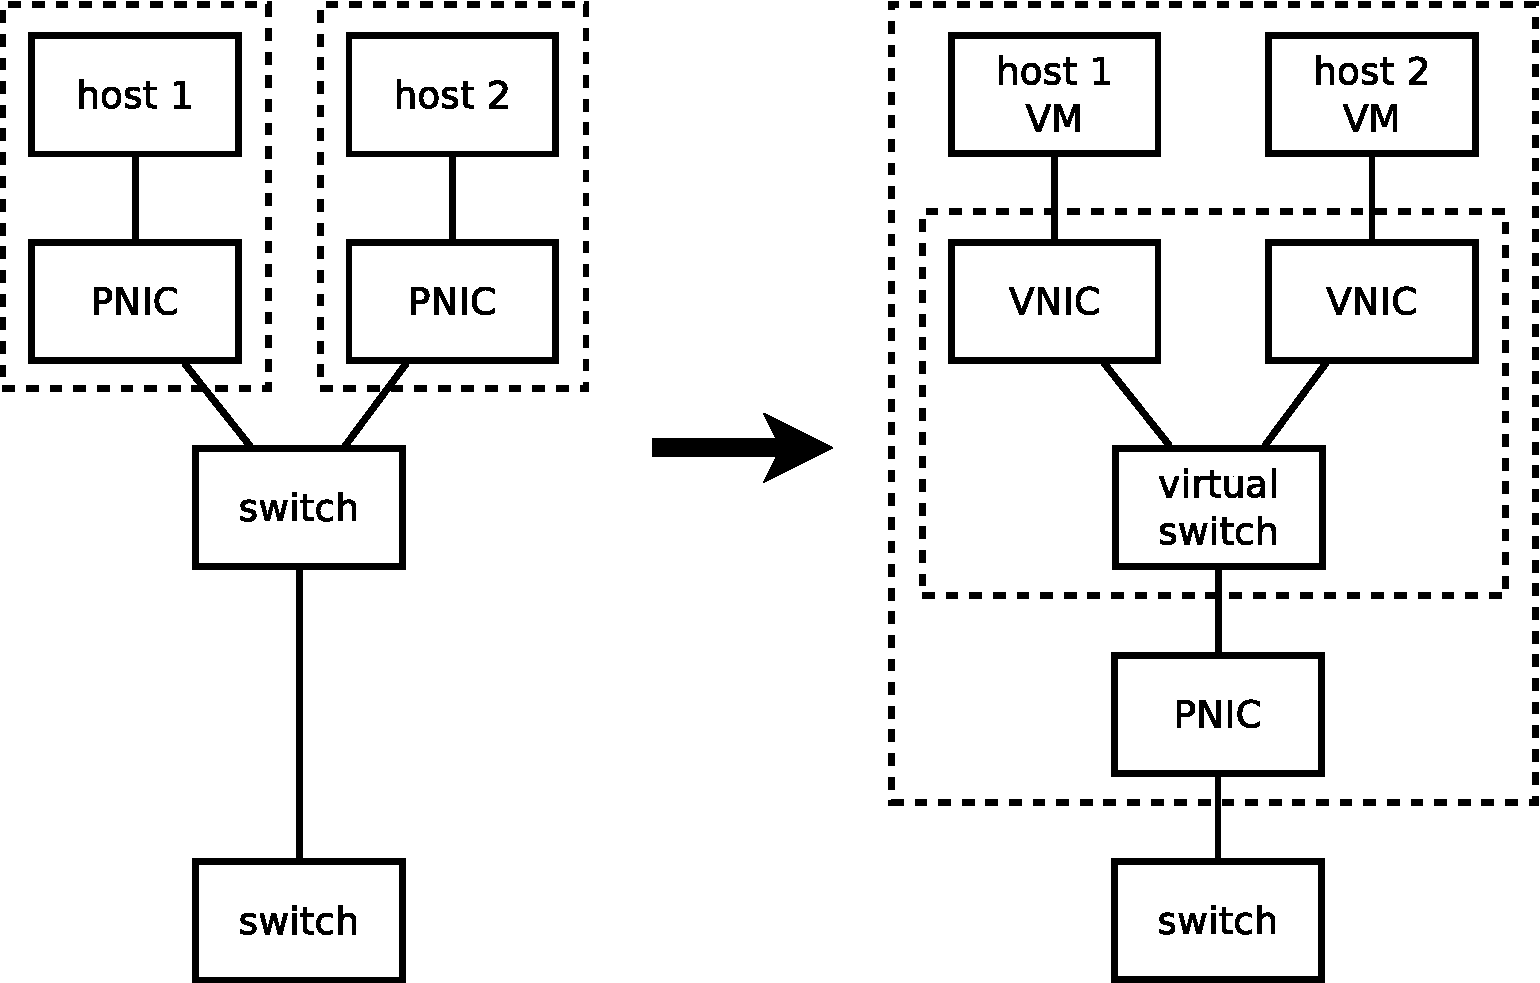
\includegraphics[width=.7\textwidth]{img/solaris/mapping.pdf}

          \caption{Mapping between physical and virtual network building elements}
        \end{figure}
        
        Semantics assured by virtual switches is the same as provided by physical switches: 

        \begin{enumerate}
          \item \gls{acr:vnic}s created on top of the same \gls{acr:nic} can send packets to each other,
          \item Broadcast packets received by the underlying \gls{acr:nic} are distributed to every single
                \gls{acr:vnic} that was defined on the top of this \gls{acr:nic},
          \item Broadcast packets sent by one of the \gls{acr:vnic}s is distributed to all \gls{acr:vnic}s defined on
                the top of the same \gls{acr:nic} and to the \gls{acr:nic} for further transmission as well,
          \item In terms of multicast network traffic multicast group membership is monitored and used for distributing
                packets to appropriate \gls{acr:vnic}.
        \end{enumerate}

        Data Link Layer connectivity between \gls{acr:vnic}s is available only when they were defined on top of the same
        \gls{acr:nic} \cite{crossbow2}. 

	
      \subsection{Crossbow components}

        The Crossbow specification describes three major components: \gls{acr:vnic}s, Etherstubs and Flows. This section
        gives an insight into their application and usage.

                
        \subsubsection{VNICs}
        
          \gls{acr:vnic}s each containing their own lane are the key element in crossbow architecture. There is no
          difference between \gls{acr:nic} and \gls{acr:vnic} in administration, as they are all treated as data links.
          Every \gls{acr:vnic} has an assigned lane and flow classifier which classifies received packets by
          \gls{acr:vnic}'s MAC address and sometimes by the \gls{acr:vlan} tag.  If created with a \gls{acr:vlan} tag,
          protocols like \gls{acr:gvrp} or \gls{acr:mvrp} may be used to register the \gls{acr:vlan} tag with the
          physical switches too \cite{crossbow}.	

          In terms of sharing bandwidth, Crossbow enables administrative control of bandwidth for every single
          \gls{acr:vnic}. The bandwidth of the link is implemented by regulating the periodic intake of incoming packets
          per dedicated lane. The network stack allows only as many packets as it was assigned to specific
          \gls{acr:vnic}. The lane picks more packets when the next period begins. In case of regulating the speed of
          transmitted bandwidth it is much easier as the network stack can either control the application that is
          generating the stream of packets or just drop the excessive amount of packets. These mechanisms are also used
          in flows \gls{acr:qos} described and discussed later in this paper \cite{crossbow}.


        \subsubsection{Etherstubs}

          As it was mentioned before, the MAC layer provides the virtual switching capabilities which allow
          \gls{acr:vnic}s to be created over existing physical \gls{acr:nic}s.  In some cases, creating virtual networks
          without the use of a physical \gls{acr:nic} is more welcomed than creating over physical \gls{acr:nic}s. In
          that case \gls{acr:vnic}s would be defined on the top of pseudo \gls{acr:nic}s.  The Crossbow provides these
          kind of elements which are called Etherstubs. These components could be used instead of \gls{acr:nic}s during
          creation of \gls{acr:vnic}s \cite{crossbow}.


        \subsubsection{Flows}

          Flows are additional instruments created to allow easier network traffic administration. They might be used in
          order to provide bandwidth resource control and priority for protocols, services, containers. Virtual networks
          can be described to maintain isolation and different network properties, and define flows to manage quality of
          service \cite{network_virtualization}.

          Defined flow is a set of attributes based on Layer 3 and Layer 4 headers of the \gls{acr:osi} model which are
          then used to identify protocol, service or virtual machine. Flows assigned to a link must be independent
          therefore before adding new one its correctness is checked. Input and output packets are matched to flows in
          very efficient manner with minimal performance impact.

          \medskip

          Crossbow flows can be created with one of the following sets of attributes:

          \begin{itemize}
            \item Services (protocol + remote/local ports),
            \item Transport (TCP, UDP, SCTP, iSCSI, etc),
            \item \gls{acr:ip} addresses and \gls{acr:ip} subnets,
            \item \gls{acr:dscp} field.
          \end{itemize}

          For each flow the following properties can be set \cite{flows2}: 

          \begin{itemize}
            \item bandwidth,
            \item priority.
          \end{itemize}

          \textbf{flowadm} is the console command used to create, modify, remove or to display network bandwidth and
          priority limits assigned to a particular link. 


      \subsection{Running examples of flowadm and dladm command}

        \textbf{dladm} and \textbf{flowadm} are two basic administrative commands for dealing with the Crossbow's
        components. Below a few general examples of their usage are presented.
  
        \textbf{dladm} is the admin command for crossbow datalinks elements management. Below a few examples of
        \gls{acr:vnic}s, Etherstubs management commands are presented and how bandwidth and priority values might be
        assigned to these elements. \\


        \noindent
        \begin{minipage}{\textwidth}
          \lstinputlisting[caption={\textbf{dladm} command usage examples},label={lst:uc:xbow:dladm}]{lst/dladm.sh}
        \end{minipage}
  
        More examples can be found in \textbf{man dladm}. \\


        \textbf{flowadm} is the admin command for flow management. It might be used as follows: \\

        \noindent
        \begin{minipage}{\textwidth}
          \lstinputlisting[caption={\textbf{flowadm} command usage examples},label={lst:uc:xbow:flowadm}]{lst/flowadm.sh}
        \end{minipage}

        More information about \textbf{flowadm} and \textbf{dladm} available options can be found in manual.

      \subsection{Creating zone over VNIC}

        Listing \ref{lst:uc:xbow:vnic-zone} shows an example of assigning \gls{acr:vnic} to zones. Exclusive
        \gls{acr:ip} zones must be used when zones are to be used as containers for the virtual network. \\

        \noindent
        \begin{minipage}{\textwidth}
          \lstinputlisting[caption={Creating an Exclusive IP Zone Over a VNIC example},label={lst:uc:xbow:vnic-zone}]{lst/vnic-zone.sh}
        \end{minipage}


      \subsection{Crossbow and Differentiated Services - interoperability}
      \label{sub:sol:diffserv}

        The Crossbow technology is designed to work inside single operating system instance, there are no mechanisms
        meant to cope with problems that arise when dealing with installations spanning multiple physical machines
        connected with traditional (non-virtual) network. Crossbow's flows are, by design, relatively simple (when
        compared to DiffServ) but more efficient as far as receive performance is considered \cite{xbow-vertically}.
        Crossbow, unlike DiffServ, does not require special hardware, although if it is present it can boost overall
        operation performance \cite{xbow-vertically}.

        DiffServ, on the other hand, provides sophisticated \gls{acr:qos} mechanisms that require proper hardware
        (DiffServ-aware routers) to be present for it to work. DiffServ is standardized (\gls{acr:rfc} 2475) and offers
        a multiplicity of classification, marking, policing and traffic shaping alternatives \cite{rfc2475}. Special
        fields (called \gls{acr:dscp}) contained in \gls{acr:ip} packet's header are used to carry processing-related
        information with packets. The approach can be used with complex networks, comprising a number of routers with
        \gls{acr:qos} awareness.

        These two environments complement one another rather than compete. Crossbow supports flow matching based on the
        \gls{acr:dscp} field value. \gls{acr:dscp} field generation is planned but not yet supported. It is possible
        (although, at the moment, only partially) to integrate these and build a comprehensive end-to-end networking
        solution with \gls{acr:qos} support and virtualized components.

        \begin{figure}[H]
          \begin{center}
            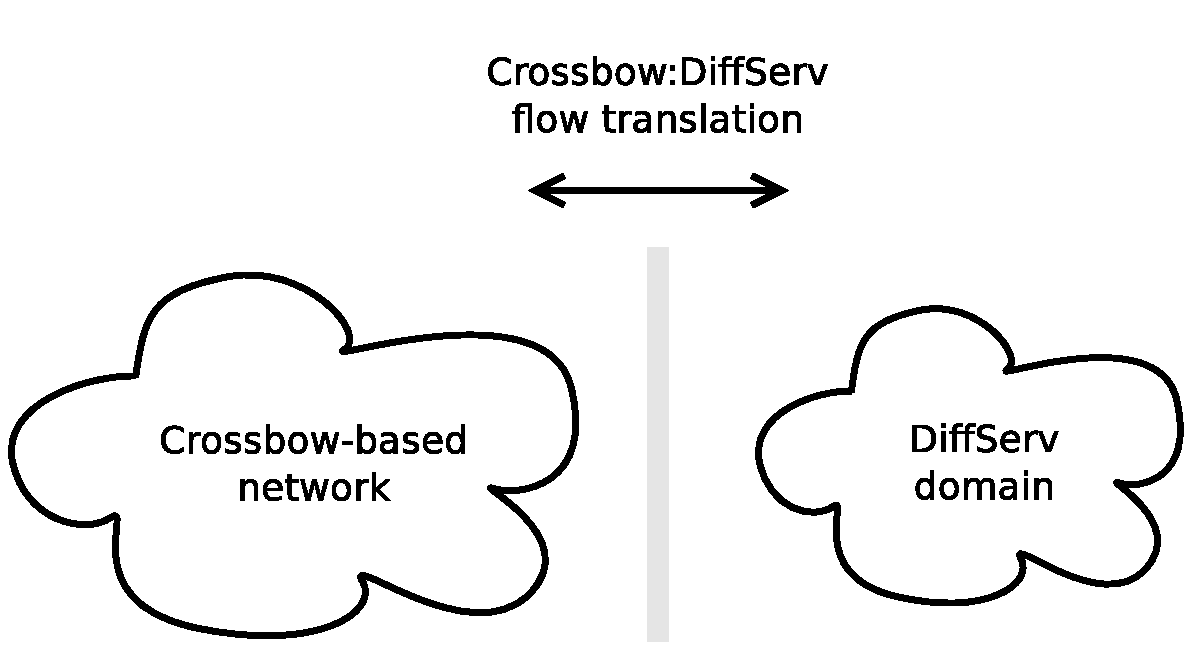
\includegraphics[width=.7\textwidth]{img/solaris/xbow-diffserv.pdf}
          \end{center}

          \caption{DiffServ integration using Crossbow-provided mechanisms}
        \end{figure}


    \section{Resource control}
    \label{sec:sol:res}

      Nowadays existing operating systems must provide mechanisms for response to the varying resource demands per
      workload which is an aggregation of processes of an application. By default resource management features are not
      used and system gives equal access to resources. When necessary, it is possible to modify this default behaviour
      with respect to different workloads. It is allowed to:

      \begin{enumerate}
        \item Restrict access to specific resource,
        \item Offer resources to workloads on a preferential basis,
        \item Isolate workloads from each another.
      \end{enumerate}
	
      Resource is any part of computing system that may be modified in order to change application behaviour. Resource
      management enables more effective resource utilization and avoid wasting available ones due to load variability.
      Reserving additional capability during off-peak periods and effective sharing resources definitely increases
      application performance \cite{oracle_admin_guide}.

      Most of the operating systems limited the resource control just to per-process control, whereas Oracle Solaris has
      extended this concept to the task, project and zone. Due to introducing granularity levels processes, tasks, and 
      zones are efficiently controlled from excessive resource consumption. All these enhacements are available thanks 
      to resource controls (rctls) facility \cite{oracle_admin_guide}.
      
      Solaris Operating System introduced three types of resource management control mechanisms:

      \begin{enumerate}
        \item constraints --- allows defining set of bounds on used resources for a workload,
        \item partitioning --- enables binding subset of system's available resources to specific workload,
        \item scheduling --- involves predictable algorithm making sequence of allocation decisions at specific
                             intervals.
      \end{enumerate}

      Hierarchical architecture allows defining set of resource control sets on each level. However, if more than one is
      assigned to a resource, the smallest container's control level is enforced \cite{oracle_admin_guide}. 

      \begin{figure}[H]
        \centering
        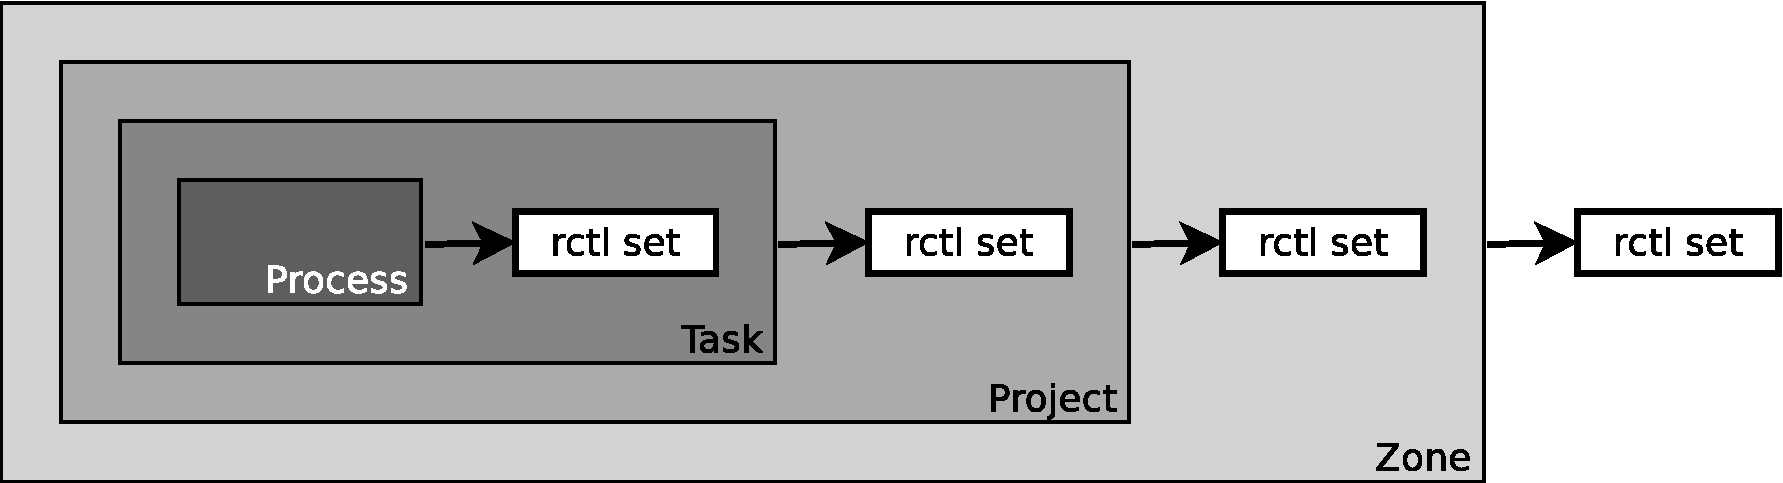
\includegraphics[width=.7\textwidth]{img/solaris/multi.pdf}

        \caption{Solaris system multilevel architecture and its resource control sets}
		  \end{figure}


      \subsection{Accounting}
      \label{sub:sol:acct}

        Highly configurable accounting facility is provided as part of the system. Its role is to gather historical
        usage records of system and network resources. There are two levels accounting can work on in Solaris
        OS - basic and extended. Basic accounting allows for per-zone and per-project statistics gathering while
        extended accounting facility makes it possible to collect the data for tasks and processes. Statistics gathered
        by the extended accounting can be examined using C or Perl interface of the libexacct library \cite{sag}.

        The extended accounting facility can gather data for:

        \begin{itemize}
          \item system resources usage (per-task and per-process),
          \item flows defined with the IPQoS tools,
          \item links and flows created with Crossbow.
        \end{itemize}

        % TODO what data can be gathered?


    \section*{Summary}

      The chapter presented the Solaris operating system with regard to resource virtualization. The stack of tools
      integrated into the system provides an extensive support for virtualization techniques: Containers facilitate
      OS-level resource virtualization and Crossbow, shipped with Solaris 11, makes virtualization of networking
      resources possible. Resource control subsystem gives the administrator even more fine-grained control over
      resource utilization. Last but not least, accounting functionality provides a detailed view of the resource usage
      history.

      The features mentioned above make the realization of flexible, scalable and efficient systems possible. With these
      foundations, it is possible to build and consolidate complex network-oriented infrastructures that prove to be
      reliable, relatively easy to manage and adjust to changing requirements.

      Solaris 10 OS seems to be an ideal cross-platform choice for customers dealing with the management of high level
      services, complex system administration and high costs. It is the only open operating system which has proven
      results running from every critical enterprise databases to high performance Web farms. That is why Solaris OS is
      becoming strategic platform for today's constantly growing demands on operating systems
      \cite{solaris_operating_system}. 


  \chapter{The CM4J system architecture}
  \label{chap:arch}

    The chapter discusses architectural aspects of the created system. First, the operating environment is discussed
    together with third-party components used to run the system. Then, general high-level view is described and
    layers of the system are presented. The remaining sections describe details of the layers.

    Section \ref{sec:arch:env} presents the context of the system. The distributed environment is described and
    basic requirements with regard to installed software are listed. Also, the way of extending the environment with
    specialized components is presented.

    Section \ref{sec:arch:over} introduces the design of the system. Main layers (or subsystems) are identified together
    with corresponding responsibilities. General aspects of layer interoperability are described.

    Section \ref{sec:arch:inst} provides in-depth description of resource instrumentation layer. Its internal design is
    presented and main classes of objects analyzed. Interactions between the objects are depicted and, finally, the
    listing showing all the crucial classes belonging to the layer follows.

    Section \ref{sec:arch:vi} describes the topmost layer of the whole system --- virtual infrastructure management. The
    layer functionality is presented, then data model used is introduced and discussed and main components of the layer
    are described together with their interdependencies and interactions. Extensive description of the layer's three
    main use-cases --- instantiation, discovery, monitoring --- follows.


    \section{Operating environment}
    \label{sec:arch:env}

      As depicted in figure \ref{fig:arch:deployment}, the system is designed to operate in a distributed environment
      --- the bottommost layer of the operating environment is an \gls{acr:ip} network of physical machines. Each of the
      machines is running an instance of Solaris Operating System with support for Crossbow technology. None of the
      nodes is favoured over the others. The instances of operating system have \gls{acr:jvm} deployed and are capable
      of running \gls{acr:jmx} Agent which is used to host components of the system.

      In addition to these basic specification, pure \gls{acr:jmx} Agents (i.e. agents without any components registered) can be
      enriched with third-party software and thus enable complete set of functionality implemented. With pure \gls{acr:jmx} Agents
      only single-node management is possible and limited to Crossbow networking resources. After integration with \gls{acr:jims}
      the system gains awareness of the whole distributed environment, has access to extensive mechanisms for
      controlling containers and can be used to create and manage complex virtual network topologies.
    
      \begin{figure}[H]
        \begin{center}
          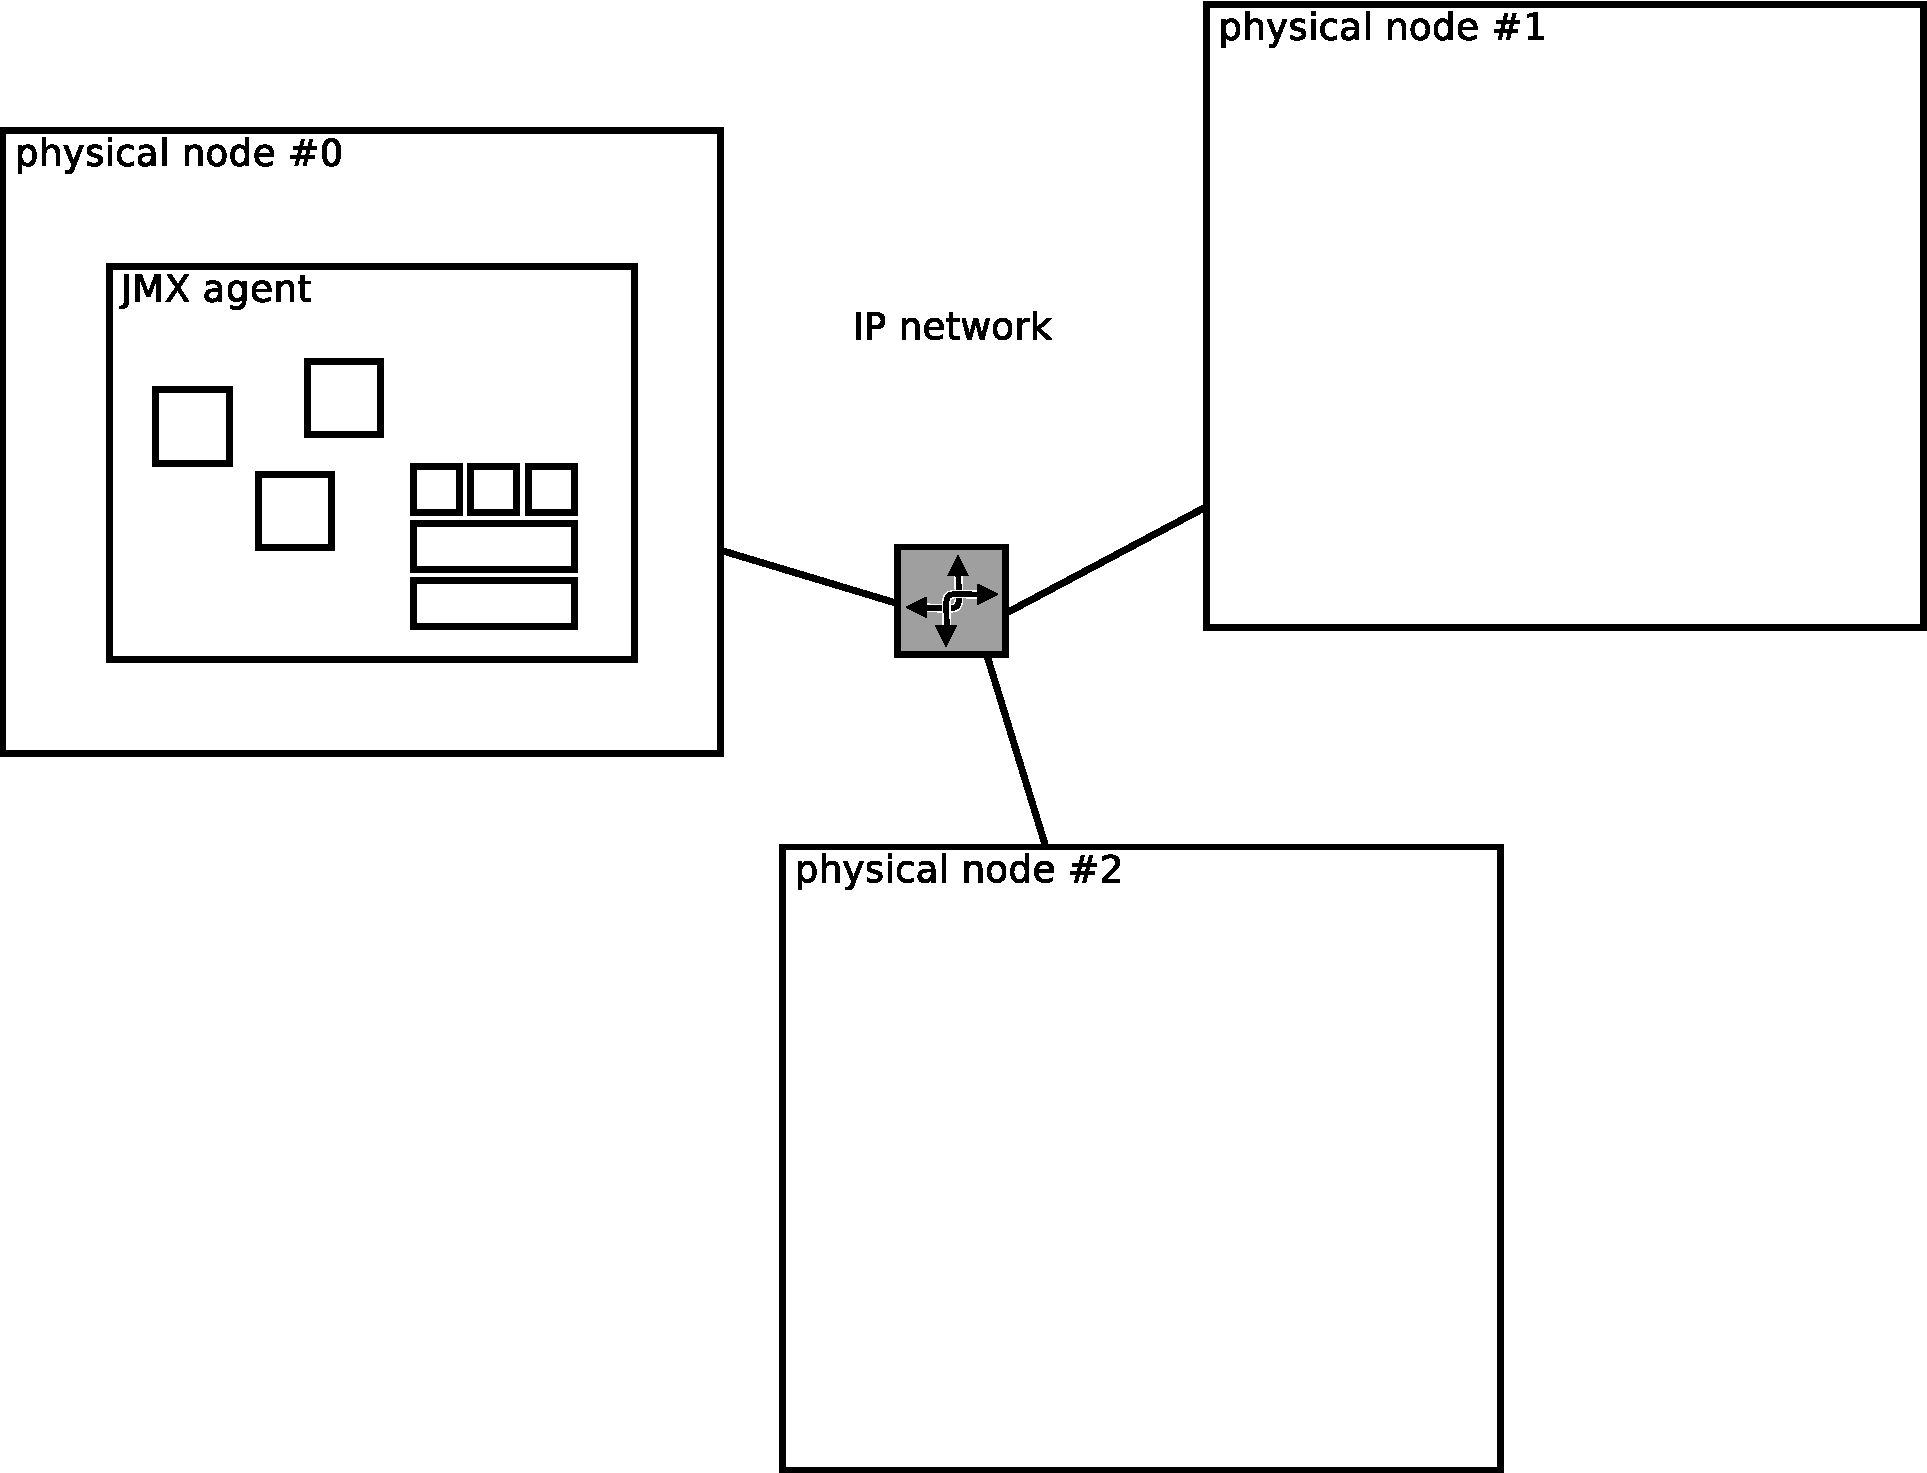
\includegraphics[width=.8\textwidth]{img/architecture/deployment.pdf}
        \end{center}

        \caption{Deployment diagram for the system}
        \label{fig:arch:deployment}
      \end{figure}


    \section{Architecture overview}
    \label{sec:arch:over}

      When considered at a very high level, the architecture of the system as a whole is layer-based. There are three
      main layers, each specifying a set of its own interfaces. The higher the layer is placed in the stack, the more
      complex interface it exposes. The three layers, as shown in figure \ref{fig:arch:layers}, are:

      \begin{itemize}

        \item Infrastructure management layer

              contains components that help design, instantiate and manage network topologies, \\
              can possibly span multiple physical machines, \\
              requires \gls{acr:jims} installation to operate,

        \item Resource instrumentation layer

              is an abstraction layer over resources provided by the underlying system, \\
              present on each of the physical hosts, \\
              network-based interoperability between nodes is not supported,

        \item Underlying resources layer

              represents all the resources made available by host operating system, \\
              can be managed with vendor-supplied low-level utilities and libraries.

      \end{itemize}

      All the operations (e.g. topology modification) performed by infrastructure management layer go down the stack
      and, after necessary transformations, result in persistent changes to underlying resources. Conversely, the state
      of low-level resources can be expressed in terms of the domain model used by the highest layer (discovery
      process).

      \begin{figure}[H]
        \begin{center}
          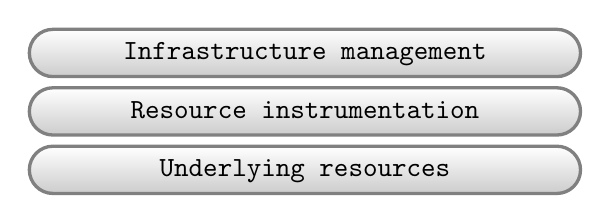
\begin{tikzpicture}[start chain,
                              node distance=1mm,
                              every node/.style={terminal, minimum width=7cm},
                              text depth=.25ex]

            \node (infr)                 {Infrastructure management};
            \node (inst) [below=of infr] {Resource instrumentation};
            \node (undr) [below=of inst] {Underlying resources};
          \end{tikzpicture}
        \end{center}

        \caption{Layered system architecture}
        \label{fig:arch:layers}
      \end{figure}


    \section{Crossbow resources instrumentation}
    \label{sec:arch:inst}

      The main responsibility of resource instrumentation subsystem is to provide a consistent way to create and manage
      resources of the underlying operating system. This general-purpose abstraction layer can easily be expanded when
      needed and further leveraged to build more sophisticated systems on top of it.


      \subsection{Separation of concerns}

        There are two classes of objects present at this level (figure \ref{fig:arch:manent}) --- Entity objects that
        are abstractions representing resources of specific type and exposing appropriate interfaces, and Manager
        objects used to perform basic coarse-grained operations (such as creation, deletion, modification) on resources
        they manage.

        \begin{figure}[H]
          \begin{center}
            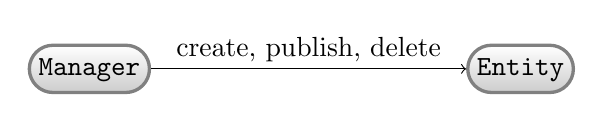
\begin{tikzpicture}[node distance=4cm, text depth=.25ex]

             \node (ent) [terminal] {Entity};
             \node (man) [terminal, left=of ent] {Manager}
               edge [->] node [auto] {create, publish, delete} (ent);

            \end{tikzpicture}
          \end{center}

          \caption{Manager and entity objects interoperability}
          \label{fig:arch:manent}
        \end{figure}


        \subsubsection{Entity objects}

          Entity objects represent instances of a resource type. Each entity object class exposes an interface to manage
          the resource it is associated with. Fine-grained management is possible with entity objects --- single
          properties can be accessed and manipulated (a subset of Flow public interface is presented in listing
          \ref{lst:arch:iface:flow}). \\

          \noindent
          \begin{minipage}{\textwidth}
            \lstinputlisting[caption={Selected methods of entity interface},label={lst:arch:iface:flow},language=Java]{lst/arch-iface-flow.java}
          \end{minipage}


        \subsubsection{Manager objects}

          Each manager subtype is associated with a single class of resources. The subtype can be thought of as a
          gateway exposing methods to manage collection of resources. The responsibilities of manager objects include
          resource discovery, creation, modification and removal. Managers maintain lists of resources present in the
          system and provide ways to access them (as entity objects). The resources can also be published in external
          repositories. \\

          \noindent
          \begin{minipage}{\textwidth}
            \lstinputlisting[caption={Selected methods of manager interface},label={lst:arch:iface:flowmanager},language=Java]{lst/arch-iface-flowmanager.java}
          \end{minipage}

          Sequence diagram in figure \ref{fig:arch:pub} shows the process of creating new entity object. After creation,
          the object is published in a repository to make it accessible for other components.

          \begin{figure}[H]

            \centering

            \begin{tikzpicture}[text height=1.5ex, text depth=.25ex]
              
              \begin{umlseqdiag}

                \umlobject{Client}
                \umlobject{Manager}
                \umlobject{Native library}
                \umlobject{Publisher}

                \begin{umlcall}[op={create(entity)}]{Client}{Manager}
                  \begin{umlcall}[op={create(entity)}]{Manager}{Native library}
                  \end{umlcall}
                  \begin{umlfragment}[inner ysep=2]
                    \begin{umlcall}[op={publish(entity)}, return=id]{Manager}{Publisher}
                    \end{umlcall}
                  \end{umlfragment}
                \end{umlcall}
              
              \end{umlseqdiag}
            
            \end{tikzpicture}

            % \begin{sequencediagram}

            %   \newthread{cli}{Client}
            %   \newinst[2]{man}{Manager}
            %   \newinst[1]{lib}{Native library}
            %   \newinst[1]{pub}{Publisher}

            %   \begin{call}{cli}{create(entity)}{man}{}
            %     \begin{call}{man}{create(entity)}{lib}{}
            %     \end{call}
            %     \begin{sdblock}{if publisher attached}{}
            %       \begin{call}{man}{publish(entity)}{pub}{id}
            %       \end{call}
            %     \end{sdblock}
            %   \end{call}
            % 
            % \end{sequencediagram}

            \caption{Entity creation scheme with optional publication}
            \label{fig:arch:pub}
          
          \end{figure}


      \subsection{Layered design}

        Both the Manager and Entity objects share the same three-layer internal design as presented in figure
        \ref{fig:arch:laydes}. The objects themselves are exposed as \gls{acr:jmx} beans. To implement the interface,
        either shell scripts or native libraries (or both) are used depending on the complexity of an operation. At the
        lower level, command line programs or native calls are executed, respectively.

        \begin{figure}[H]
          \begin{center}
            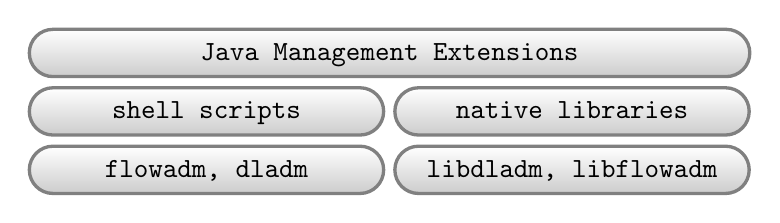
\begin{tikzpicture}[start chain,
                                node distance=1mm,
                                every node/.style={terminal, minimum width=4.5cm},
                                text height=1.5ex, text depth=.25ex]

              \node (jmx)  [minimum width=9.15cm] {Java Management Extensions};
              \node (midl) [below=of jmx.south west, anchor=north west] {shell scripts};  \node (midr) [right=of midl] {native libraries};
              \node (lowl) [below=of midl] {flowadm, dladm};                              \node (lowr) [right=of lowl] {libdladm, libflowadm};
            \end{tikzpicture}
          \end{center}

          \caption{Layered system architecture}
          \label{fig:arch:laydes}
        \end{figure}


      \subsection{Instrumented Solaris OS resources}

        All the important Crossbow resources are instrumented (Manager:Entity pairs are created). This includes
        \gls{acr:nic}s, \gls{acr:vnic}, \gls{acr:vlan}, Etherstubs and Flows. All the components are loosely coupled and
        can be used independently.

        \begin{figure}[H]
          \begin{center}
            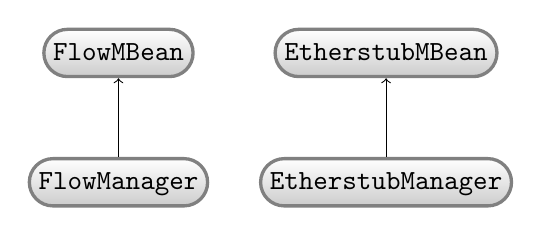
\begin{tikzpicture}[every node/.style={minimum width=4.5cm},
                                text height=1.5ex, text depth=.25ex]

              \node (eflow) [terminal] {FlowMBean};
              \node (mflow) [terminal, below=of eflow] {FlowManager};

              \node (eether) [terminal, right=of eflow] {EtherstubMBean};
              \node (mether) [terminal, below=of eether] {EtherstubManager};

              \useasboundingbox (current bounding box);

              \path [->] (mflow)  edge node [auto] {manages} (eflow)
                         (mether) edge                       (eether);

            \end{tikzpicture}

            \bigskip

            \begin{tikzpicture}[every node/.style={minimum width=4.5cm},
                                text height=1.5ex, text depth=.25ex]

              \node (enic) [terminal, below=of mflow] {NICMBean};
              \node (mnic) [terminal, below=of enic] {NICManager} (enic);

              \node (evnic) [terminal, right=of enic] {VNICMBean};
              \node (mvnic) [terminal, below=of evnic] {VNICManager}
                edge [->] node [auto] {} (evnic);

              \node (evlan) [terminal, right=of evnic] {VLANMBean};
              \node (mvlan) [terminal, below=of evlan] {VLANManager};

              \useasboundingbox (current bounding box);

              \path [->] (mnic)  edge node [auto] {manages} (enic)
                         (mvnic) edge                       (evnic)
                         (mvlan) edge                       (evlan);
              
            \end{tikzpicture}
          \end{center}

          \caption{Instrumented resources}
          \label{fig:arch:instr}
        \end{figure}
        

    \section{Virtual infrastructure management}
    \label{sec:arch:vi}

      Virtual infrastructure management subsystem is built on top of the instrumentation layer. Leveraging entity and
      manager objects and components of the \gls{acr:jims} project, it provides high-level mechanisms to manage and monitor
      complex network topologies and quality policies associated with them.


      \subsection{High-level functionality overview}
      \label{sub:arch:hl}

        Figure \ref{fig:arch:hl} shows main stages of the management process together with general flows of data and is
        the starting point when identifying and designing coarse-grained components. The stages presented map to
        implemented components of the system that were implemented --- User Interface to design, manipulate and monitor
        the topology, nodes responsible for discovery of available physical hosts, and mappers which translate between
        logical model and underlying resources.

        \begin{figure}[H]
          \begin{center}
            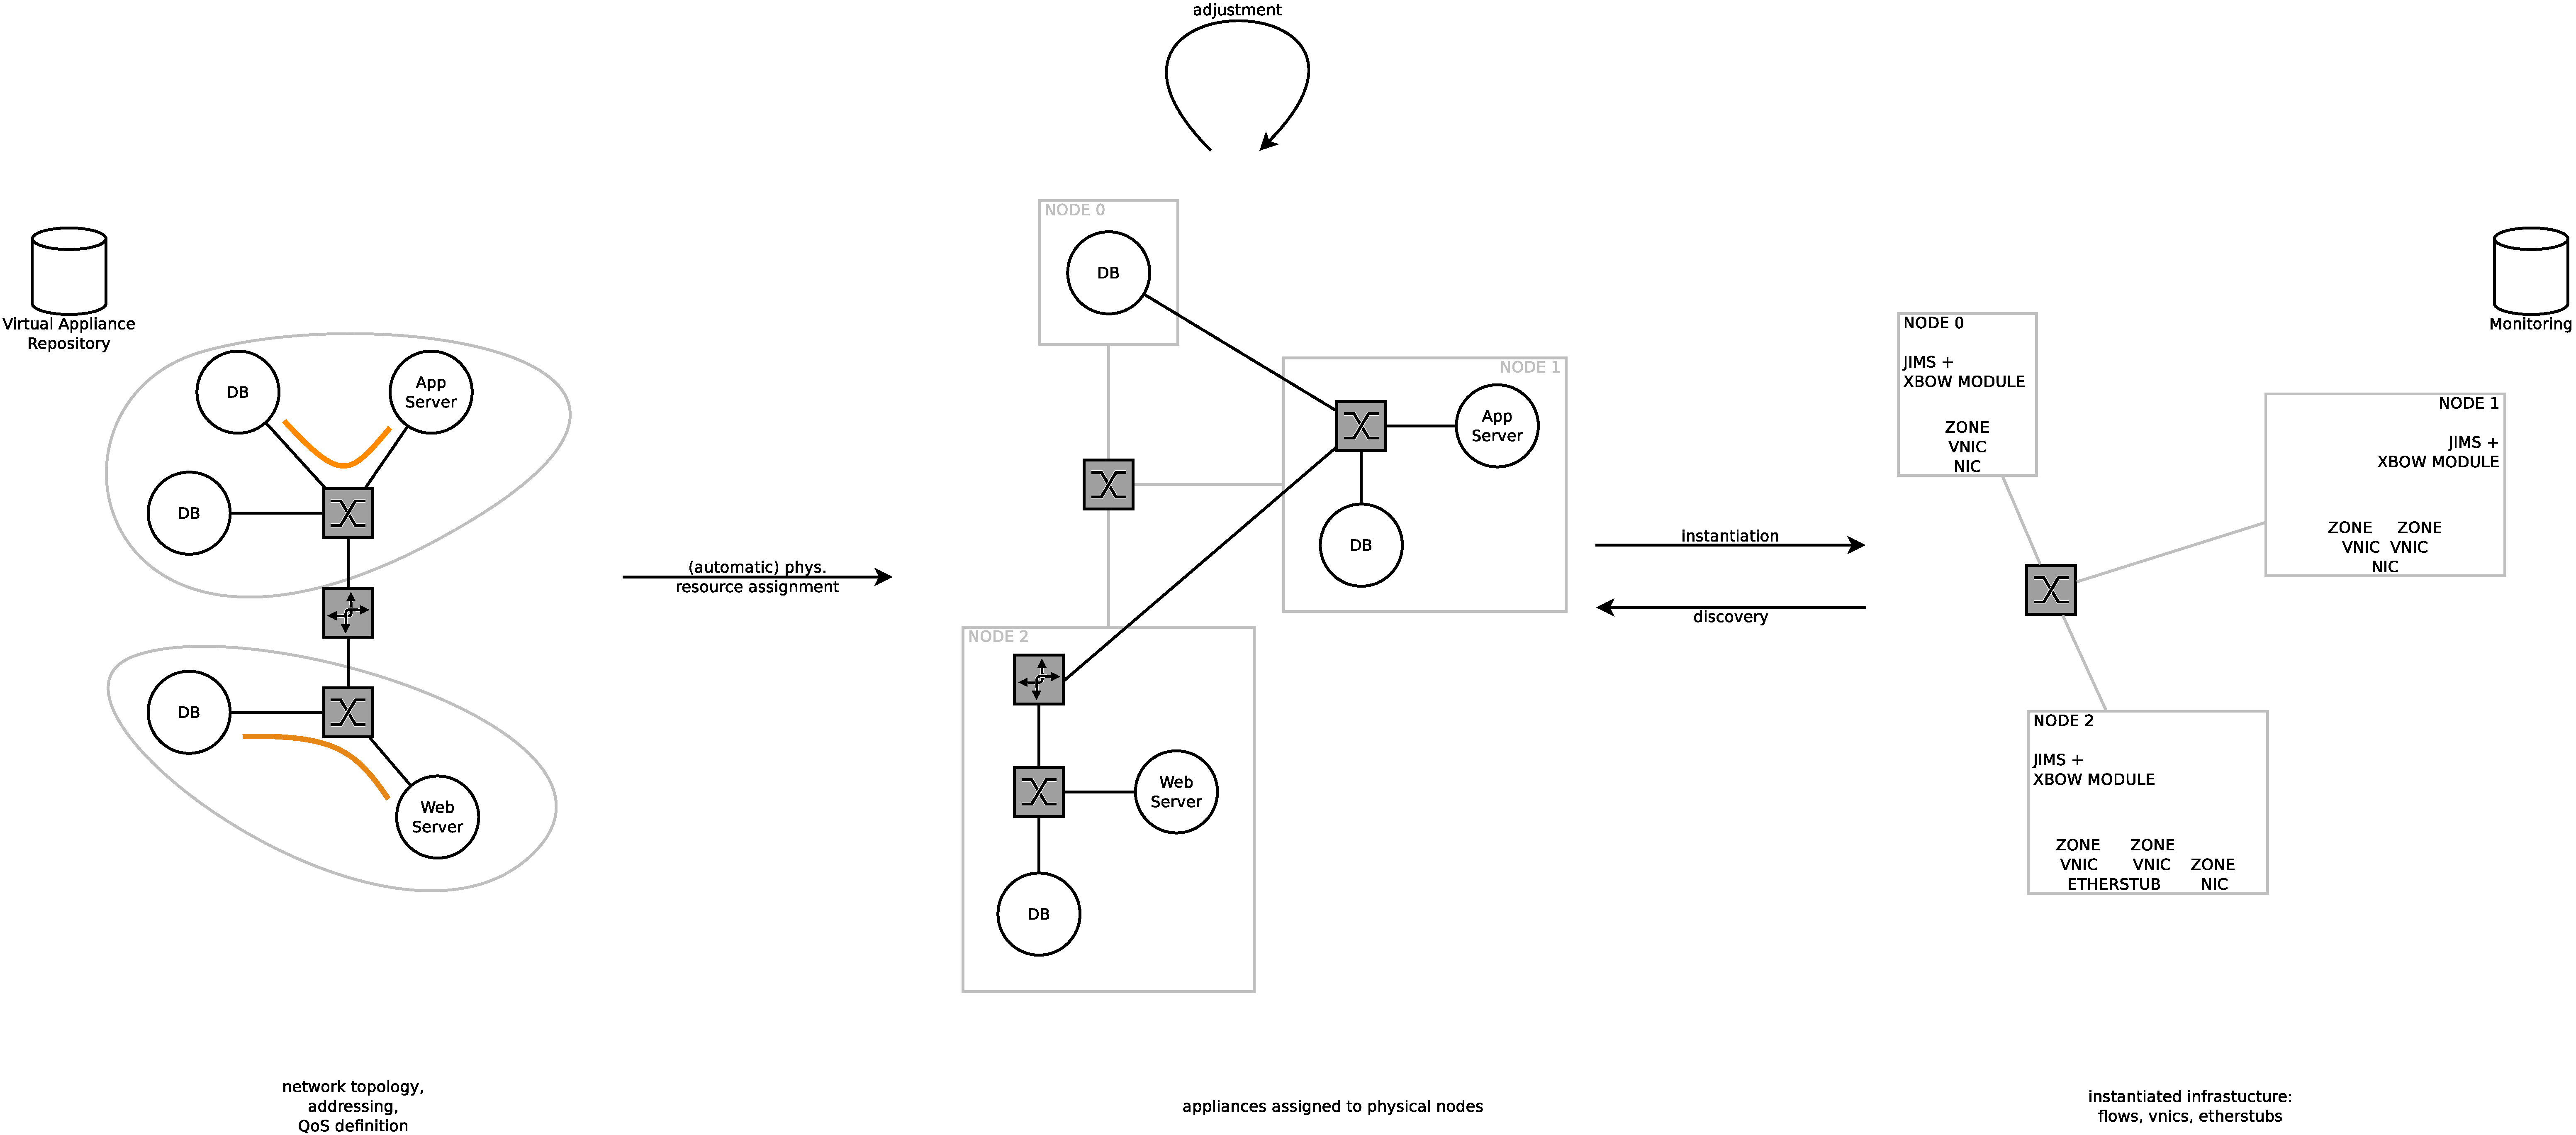
\includegraphics[width=\textwidth]{img/architecture/scope.pdf}
          \end{center}

          \caption{Main stages of operation}
          \label{fig:arch:hl}
        \end{figure}


      \subsection{Domain model and data flows}
      \label{sec:domain-model}

        Dedicated domain model was created for the virtual infrastructure management layer. It describes higher-level
        entities and operations that can be performed. The model is divided into three logical groups --- static data
        describes resources and their interdependencies, assignment model is used to denote the association between
        parts of a topology and underlying physical resources, actions model is used to express the operations that can
        be applied to elements of a topology.


        \subsubsection{Static data model}

          As far as networking domain is considered, the model covers three main aspects:

          \begin{itemize}

            \item available entities --- the set of resources that can be used to build a network topology,

                  \begin{figure}[H]
                    \centering

                    \begin{tikzpicture}
                      \umlclass{Resource}
                      {
                        + projectId : String \\
                        + resourceId : String \\
                      }
                      {}

                      \umlclass[x=-4, y=-3]{Appliance}
                      {
                        + repoId : String \\
                        + type : ApplianceType
                      }
                      {}

                      \umlclass[x=-4, y=-6]{Router}
                      {
                        + type : ApplianceType = ROUTER
                      }
                      {}

                      \umlemptyclass[x=4, y=-3]{Endpoint}

                      \umlclass[y=-8]{RoutingTable}
                      {
                        + staticRoutes : List( IpAddress, IpAddress )
                      }
                      {}

                      \umlemptyclass[x=2, y=-5]{Switch}

                      \umlemptyclass[x=6, y=-5]{Interface}

                      \umlclass[x=8, y=-8]{IpAddress}
                      {
                        + address : String \\
                        + netmask : int
                      }
                      {}

                      \umlinherit{Appliance}{Resource}
                      \umlinherit{Router}{Appliance}

                      \umlaggreg[geometry=-|]{Router}{RoutingTable}
                      \umlaggreg[geometry=-|, arg2=0..1]{Interface}{IpAddress}

                      \umlinherit{Endpoint}{Resource}
                      \umlinherit{Switch}{Endpoint}
                      \umlinherit{Interface}{Endpoint}
                    \end{tikzpicture}

                    \caption{Object model --- entities}
                  \end{figure}

            \item allowed interconnections --- reflecting a subset of real-world connections between networking
                  hardware,

                  \begin{figure}[H]
                    \centering

                    \subfloat[Interface--Endpoint interconnection]{
                      \begin{tikzpicture}
                        \umlemptyclass{Interface}
                        \umlemptyclass[x=-4]{Endpoint}

                        \umlassoc[mult2=0..1]{Interface}{Endpoint}
                      \end{tikzpicture}
                    } \hspace{.5cm}
                    %
                    \subfloat[Switch--Endpoint interconnection]{
                      \begin{tikzpicture}
                        \umlemptyclass{Switch}
                        \umlemptyclass[x=-4]{Endpoint}

                        \umlassoc[mult2=0..*]{Switch}{Endpoint}
                      \end{tikzpicture}
                    } \vspace{.5cm}
                    %
                    \subfloat[Appliance, Interface, Policy interconnection]{
                      \begin{tikzpicture}
                        \umlemptyclass{Appliance}
                        \umlemptyclass[x=4]{Interface}
                        \umlemptyclass[x=4, y=-3]{Policy}

                        \umlaggreg[mult2=*]{Appliance}{Interface}
                        \umlaggreg[mult1=1, mult2=*]{Interface}{Policy}
                      \end{tikzpicture}
                    }

                    \caption{Object model --- interconnections}
                  \end{figure}

            \item \gls{acr:qos} policies --- classify traffic and determine priorities.

                  \begin{figure}[H]
                    \centering

                      \begin{tikzpicture}
                        \umlclass[x=-1, y=1]{Policy}
                        {
                          + policyId : String
                        }
                        {}

                        \umlclass[x=-3, y=-2]{BandwidthPolicy}
                        {
                          + limit : int
                        }
                        {}

                        \umlclass[x=-3, y=-5]{PriorityPolicy}
                        {
                          + priority : LOW / MEDIUM / HIGH
                        }
                        {}

                        \umlemptyclass[x=3, y=1]{Filter}

                        \umlemptyclass[x=7, y=-2]{AnyFilter}

                        \umlclass[x=7, y=-5]{PortFilter}
                        {
                          + protocol : String \\
                          + port : int \\
                          + location : LOCAL / REMOTE
                        }
                        {}

                        \umlclass[x=7, y=-8]{TransportFilter}
                        {
                          + protocol : String
                        }
                        {}

                        \umlclass[x=7, y=-11]{IpFilter}
                        {
                          + address : String \\
                          + netmask : int \\
                          + location : LOCAL / REMOTE
                        }
                        {}

                        \umlinherit[geometry=-|]{PriorityPolicy}{Policy}
                        \umlinherit[geometry=-|]{BandwidthPolicy}{Policy}

                        \umlaggreg{Policy}{Filter}

                        \umlinherit[geometry=-|]{AnyFilter}{Filter}
                        \umlinherit[geometry=-|]{PortFilter}{Filter}
                        \umlinherit[geometry=-|]{TransportFilter}{Filter}
                        \umlinherit[geometry=-|]{IpFilter}{Filter}
                      \end{tikzpicture}

                    \caption{Object model --- policies}
                  \end{figure}

          \end{itemize}


        \subsubsection{Modeling assignments}

          The assignment descriptor is used together with static data model to map entities to physical nodes. The
          descriptor is created automatically or by the user before instantiating the model as well as during the
          discovery stage when it is constructed by low-level components of the implemented system.

          The annotation part of the descriptor can be used to carry additional entity-specific properties that have to
          be passed between components. It can also be used to hold auxiliary data while performing internal
          transformations of the model.

          \begin{figure}[H]
            \centering

            \begin{tikzpicture}
              \umlclass{Assignments}
              {
                + assignments : Map< Object, String > \\
                + annotations : Map< Object, Object >
              }
              {}
            \end{tikzpicture}
          
            \caption{Assignments}
          \end{figure}


        \subsubsection{Actions}

          When managing the topology, actions play crucial role --- they describe, for each element of the model, the
          operation that is going to be performed. Actions are assigned not globally for the model but on per-object
          basis --- the approach that introduces more flexibility and efficiency.

          There are four types of actions designed. The object in the model can be created (ADD, as in instantiation
          phase), deleted (REM, typically performed after topology discovery), modified (UPD, for entities that support
          on-line property adjustment) or no action can be taken at all (NOOP).

          \begin{figure}[H]
            \centering

            \begin{tikzpicture}
              \umlclass{Action}
              {
                + op : ADD / REM / UPD / NOOP \\
                + resource : Resource
              }
              {}
            \end{tikzpicture}
          
            \caption{Actions}
          \end{figure}


      \subsection{System components and their responsibilities}

        The specific character of the system --- running in a distributed environment, moderate complexity --- requires
        proper architectural model. The model should allow to design the elements of the system to be highly cohesive
        and maintain coupling as loose as possible. Each component has its own well-defined role and exposes a set of
        operations to interact with others.

        The components presented in figure \ref{fig:arch:comp} reflect three main stages of operation shown in
        subsection \ref{sub:arch:hl}. Boundaries were introduced to make the partition even clearer. The following
        subsections describe the components in more detail and provide listings with most important methods of exposed
        interfaces.

        \begin{figure}[H]
          \begin{center}
            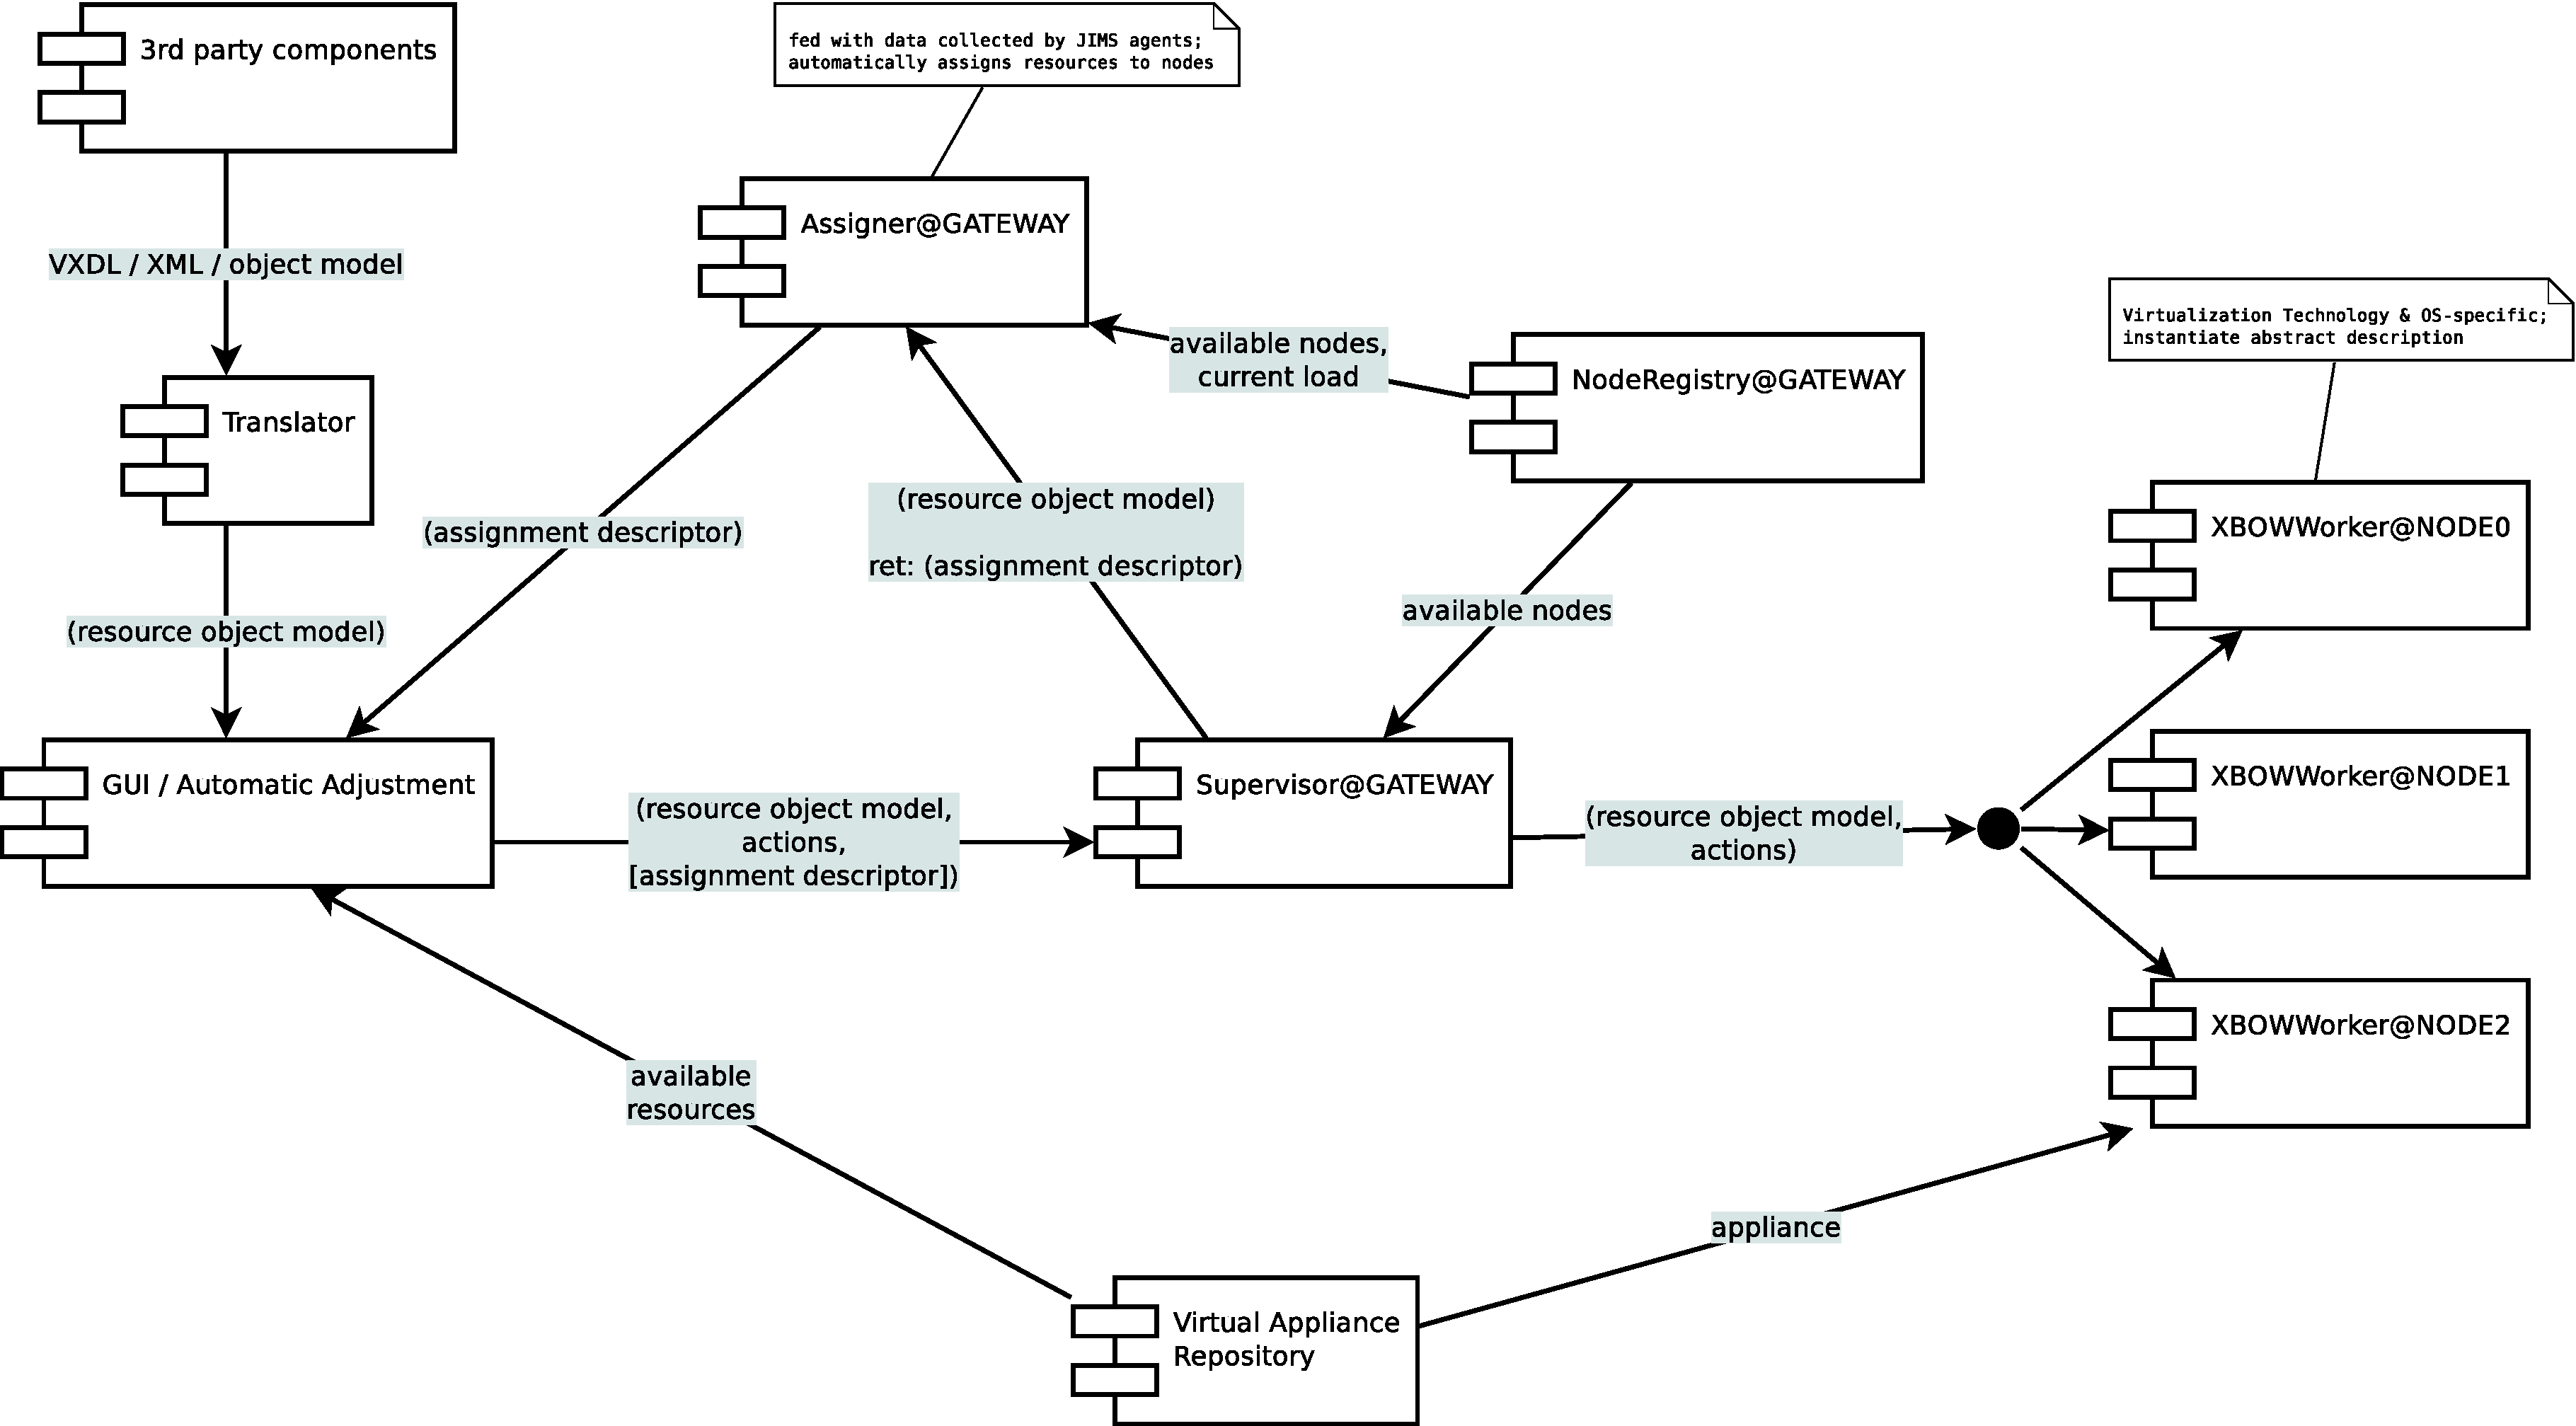
\includegraphics[width=\textwidth]{img/architecture/iaas-components.pdf}
          \end{center}

          \caption{Components of the system}
          \label{fig:arch:comp}
        \end{figure}


        \subsubsection{Virtual Appliance Repository}

          The main responsibility of Virtual Appliance Repository is to maintain the list of and provide access to
          virtual appliances created. It is used in two phases: the design phase to select appliances that are to be
          deployed, and instantiation phase to serve virtual appliance images. \\

          \noindent
          \begin{minipage}{\textwidth}
            \lstinputlisting[caption={Virtual Appliance Repository public interface},label={lst:arch:iface:repo},language=Java]{lst/arch-iface-repo.java}
          \end{minipage}
          

        \subsubsection{Assigner}

          The optional assigner module can handle entire assignment stage and make it fully automatic. To be able to do
          this, it has to be configured with a set of rules and has to continuously collect data about physical nodes
          load. If the assigner component is not present, logical model has to be assigned manually to available host
          machines.


        \subsubsection{Supervisor}

          Supervisor component manages all the worker nodes present in the system. Its responsibility is to perform
          preliminary model transformations (if needed --- for example, when using multiple host machines), divide the
          topology model according to the assignment rules and ask appropriate worker nodes to instantiate resulting
          parts.

          Supervisor delegates most of the work to worker nodes. Transactional operations can be provided at this level
          by extending the supervisor's behaviour to rollback after one of the worker nodes fails. \\

          \noindent
          \begin{minipage}{\textwidth}
            \lstinputlisting[caption={Supervisor public interface},label={lst:arch:iface:supervisor},language=Java]{lst/arch-iface-supervisor.java}
          \end{minipage}


        \subsubsection{Worker}

          Worker components perform all the low-level operations, including model to underlying entity mapping (and vice
          versa). Workers do not transform the model in any way --- all they do is provide well-defined rules for
          instantiation (including naming schemes) and discovery. Multiple workers are managed by the supervisor.

          Public interface of worker component is presented in listing \ref{lst:arch:iface:worker}. \\

          \noindent
          \begin{minipage}{\textwidth}
            \lstinputlisting[caption={Worker public interface},label={lst:arch:iface:worker},language=Java]{lst/arch-iface-worker.java}
          \end{minipage}


      \subsection{Main data flows and cooperation of the components}

        \subsubsection{Instantiation}

          There are three main stages identified when working with the topologies. There is a purely logical one that
          does not require any knowledge of the underlying environment --- the operations involve manipulating the
          domain model to create or update the virtual topology. There is an assignment stage which results in
          association between the model and physical resources. Finally, the actual deployment takes place in model
          instantiation stage --- logical elements are mapped to low-level ones after performing necessary
          transformations.

          Instantiation is the process of transforming a logical model to fully operational virtual network. There are
          three main stages that constitute the complete process:

          \begin{enumerate}

            \item Logical model definition

              This is the first stage the user is exposed to. The main task is to create a virtual network topology
              comprising logical networking components (belonging to Layer 2 and 3 of the \gls{acr:osi} model) and
              virtual appliances --- specialized virtual machines. After the topology is created, \gls{acr:ip}
              addressing is provided and routing set up. Finally, \gls{acr:qos} policies are determined to classify and
              differentiate the traffic.

            \item Physical resource selection and assignment

              After the model is defined, it can be associated with underlying physical resources. There are two
              possible ways of performing the assignment --- it can be done manually with supplied utilities or special
              component can suggest optimal solution based on, for example, current workload and predefined set of
              rules. The latter approach is particularly useful when working with complex systems that should be able to
              adjust themselves automatically to balance the load.

            \item Model instantiation

              The final, entirely automatic, step is to map the logical model and assignments to actual components
              created on the host machines. This involves a series of transformations to adjust the model to
              capabilities of the underlying environment and satisfy other requirements like topology isolation.
                  
          \end{enumerate}

          \begin{figure}[H]

            \centering

            \begin{tikzpicture}[text height=1.5ex, text depth=.25ex]
              
              \begin{umlseqdiag}

                \umlobject{GUI}
                \umlobject{Supervisor}
                \umlobject[x=10]{Worker}
                \umlobject[x=14]{VA Repository}

                \begin{umlcall}[op={getIds()}, return={appliance IDs}]{GUI}{VA Repository}
                \end{umlcall}

                \begin{umlcall}[op={instantiate(model)}]{GUI}{Supervisor}
                  \begin{umlcallself}[op={transform(model)}, return={adjusted model}]{Supervisor}
                  \end{umlcallself}
                  \begin{umlfragment}{type=loop}
                    \begin{umlcall}[op={instantiate(parts of the model)}]{Supervisor}{Worker}
                        \begin{umlcall}[op={getAppliance(id)}, return={virtual appliance}]{Worker}{VA Repository}
                      \end{umlcall}
                    \end{umlcall}
                  \end{umlfragment}
                \end{umlcall}
              
              \end{umlseqdiag}
            
            \end{tikzpicture}

            % \begin{sequencediagram}

            %   \newthread{gui}{GUI}
            %   \newinst[2]{sup}{Supervisor}
            %   \newinst[4]{wrks}{Worker}
            %   \newinst[2]{var}{VA Repository}

            %   \begin{call}{gui}{getIds()}{var}{appliance IDs}
            %   \end{call}

            %   \begin{call}{gui}{instantiate(model)}{sup}{}
            %     \begin{callself}{sup}{transform(model)}{adjusted model}
            %     \end{callself}
            %     \begin{sdblock}{loop}{for each worker with model assigned}
            %       \begin{call}{sup}{instantiate(parts of the model)}{wrks}{}
            %         \begin{call}{wrks}{getAppliance(id)}{var}{virtual appliance}
            %         \end{call}
            %       \end{call}
            %     \end{sdblock}
            %   \end{call}
            % 
            % \end{sequencediagram}

            \caption{Topology instantiation}
          
          \end{figure}

          % TODO co rozumiemy przez topologie? (topology=layout+qos)


        \subsubsection{Discovery}

          Instantiated topology, together with applied addressing, routing table entries and quality policies, can be
          discovered, i.e. object model that describes it can be recreated. The discovery process is an inverse of
          instantiation, it is composed of three phases (as shown in figure \ref{fig:arch:seqdis}):

          \begin{enumerate}

            \item The system resources are inspected by each of the Worker nodes and parts of the model together with
                  Assignment descriptors are created independently,

            \item partial results are collected and merged by the Supervisor. Redundant data is removed and necessary
                  transformations performed,

            \item complete model is passed further (e.g. to the \gls{acr:gui} component).
          
          \end{enumerate}

          \begin{figure}[H]

            \centering

            \begin{tikzpicture}[text height=1.5ex, text depth=.25ex]

              \begin{umlseqdiag}

                \umlobject{GUI}
                \umlobject{Supervisor}
                \umlobject{Worker}

                \begin{umlcall}[op={discover()}, return=model]{GUI}{Supervisor}
                  \begin{umlfragment}{type=loop}
                    \begin{umlcall}[op={discover()}, return={parts of the model}]{Supervisor}{Worker}
                    \end{umlcall}
                  \end{umlfragment}
                  \begin{umlcallself}[op={merge(parts of the model)}, return={model}]{Supervisor}
                  \end{umlcallself}
                \end{umlcall}
              
              \end{umlseqdiag}

            \end{tikzpicture}

            % \begin{sequencediagram}

            %   \newthread{gui}{GUI}
            %   \newinst[2]{sup}{Supervisor}
            %   \newinst[4]{wrk}{Worker}

            %   \begin{call}{gui}{discover()}{sup}{model}
            %     \begin{sdblock}{loop}{for each worker}
            %       \begin{call}{sup}{discover()}{wrk}{parts of the model}
            %       \end{call}
            %     \end{sdblock}
            %     \begin{callself}{sup}{merge(parts of the model)}{model}
            %     \end{callself}
            %   \end{call}
            % 
            % \end{sequencediagram}

            \caption{Topology discovery}
            \label{fig:arch:seqdis}
          
          \end{figure}


        \subsubsection{Monitoring}

          Topology operation can be monitored with high degree of granularity. Single flows can be inspected to see the
          amount of data transferred. Historical data is also made available.

          The StatisticsGatherer component performs the translation between domain models, for example it is able to map
          Policy to corresponding Flow and retrieve traffic statistics. The operation in shown in figure
          \ref{fig:arch:seqmon}.

          \begin{figure}[H]
            \centering

            \begin{tikzpicture}[text height=1.5ex, text depth=.25ex]

              \begin{umlseqdiag}

                \umlobject{GUI}
                \umlobject{StatisticsGatherer}
                \umlobject{Entity object}

                \begin{umlcall}[op={getStatistics()}, return=statistics]{GUI}{StatisticsGatherer}
                  \begin{umlcall}[op={getStatistics()}, return={statistics}]{StatisticsGatherer}{Entity object}
                  \end{umlcall}
                \end{umlcall}
              
              \end{umlseqdiag}

            \end{tikzpicture}

            % \begin{sequencediagram}

            %   \newthread{gui}{GUI}
            %   \newinst[2]{gat}{StatisticsGatherer}
            %   \newinst[2]{ent}{Entity object}

            %   \begin{call}{gui}{getStatistics()}{gat}{statistics}
            %     \begin{call}{gat}{getStatistics()}{ent}{statistics}
            %     \end{call}
            %   \end{call}
            % 
            % \end{sequencediagram}

            \caption{Topology monitoring}
            \label{fig:arch:seqmon}
          \end{figure}


    \section*{Summary}

      % TODO napisac tu cos sensownego

      The chapter provided the description and discussion of the system's architecture. The high-level layered design was
      presented and its advantages listed. Flexible and easily-expandable resources instrumentation layer was analyzed.
      The layer provides general-purpose abstractions over low-level system resources.  Finally, the topmost layer 
      (virtual infrastructure management) which used to build complex virtual network topologies was introduced.

      The design satisfies requirements the system has to meet and ensures an easy expansion when necessary. Thanks to low
      coupling, new components can be integrated whenever additional functionality is needed. The created system can
      scale to support large topology models deployed on a number of physical hosts preserving a small amount of time
      needed for the instantiation process.


  \chapter{The CM4J implementation}
  \label{chap:impl}

    This chapter focuses mainly on implementation details, especially on most interesting and complex problems
    encountered during the \gls{acr:cm4j} system implementation process  like integrating with \gls{acr:jims}, accessing
    low level functions, providing multiple programming models etc.

    The \gls{acr:cm4j} project's implementation structure is presented in section \ref{sec:impl:structure}, whereas
    section \ref{sec:impl:env} discusses implementation environment aspects like requested operating system,
    libraries presence or necessary programs to be built and installed. Issues like created components facilitating
    crossbow usage (\ref{sec:impl:comp}), low level function access methods (\ref{sec:impl:low}), prepared domain model
    transformation (\ref{sec:impl:model}) and adopted approach to data persistence (\ref{sec:impl:persist}) are mainly
    discussed in this section.

    Aspects like implemented system verification (\ref{sec:impl:verif}), detailed description of necessary steps for
    build completion (\ref{sec:impl:build}), load balancing problems and other potentially hard to solve issues
    (\ref{sec:impl:problems}) are described in the remaining part of this chapter.


    \section{The \gls{acr:cm4j} project's structure }
    \label{sec:impl:structure}

	The \gls{acr:cm4j} system consists of two subprojects: crossbow-gui and crossbow-jims-module. The crossbow-gui  
	based on technologies such as: Java, \gls{acr:swt} and Swing was created to facilitate working with implemented crossbow-jims-module.
	Without gui working with system would be more complex and tiring. A place in which core functionalities are conculded was crossbow-jims-module. 
	During the implementation process in order to fulfill previously listed requirements Java, \gls{acr:jmx}  and C was used 
	(more detailed description about both subprojects is provided in the following sections).

    \section{Implementation environment}
    \label{sec:impl:env}

      Project's architecture is based on \gls{acr:jmx} architecture which is a technology usually used for distributed resource
      management and control. These managed resources in \gls{acr:jmx} are represented by MBeans which are simple Java objects
      registered at MBean Server under specific ObjectName \cite{jims}.
    
      \begin{figure}[H]
        \begin{center}
          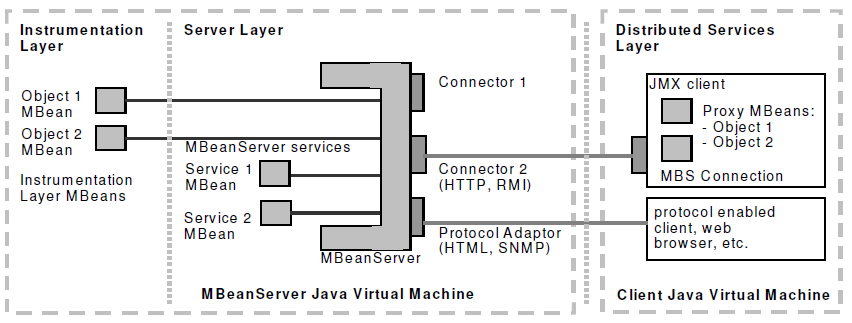
\includegraphics[width=0.9\textwidth]{img/jims/jmx.png}
        \end{center}

        % TODO przerysowac!

        \caption{JMX architecture \cite{jims}}
      \end{figure}
	
      \gls{acr:jmx} provides also services such as:

      \begin{itemize}
        \item Notifications  -- allow MBeans to send asynchronous messages which usually inform about MBean's state change, event occurrence or other important issue,
        \item MLet (downloading dynamic modules) -- allow to instantiate and register one or more MBeans in the MBean Server downloaded from remote URL.
      \end{itemize}
	
      As already mentioned the \gls{acr:cm4j} system consists of two subprojects. The implementation environment
     requirements to each of them are a bit different. 
	
      \subsection{The jims-crossbow-module implementation environment}

      In case of the jims-crossbow-module the implementation environment must consist:

      \begin{itemize}
        \item gcc compiler - for building jims-crossbow shared libraries,
        \item dladm, flowadm libraries.
      \end{itemize}
	
      The demand for crossbow libraries (flowadm, dladm) implicated that implementation environment must have been
      Solaris 11 or any other system supporting crossbow.

     Whole jims-crossbow-module was designed in order to extern existing \gls{acr:jims} system and integrate with it.

      \gls{acr:jims} supports monitoring and management under both Linux and Solaris platforms. Thanks to \gls{acr:jims}
      features such as easy maintenance (automatic modules downloading) and extensibility (possibility of adding
      additional modules) the task of integrating \gls{acr:cm4j} with \gls{acr:jims} is straightforward \cite{jims}.
    
      \begin{figure}[H]
        \begin{center}
          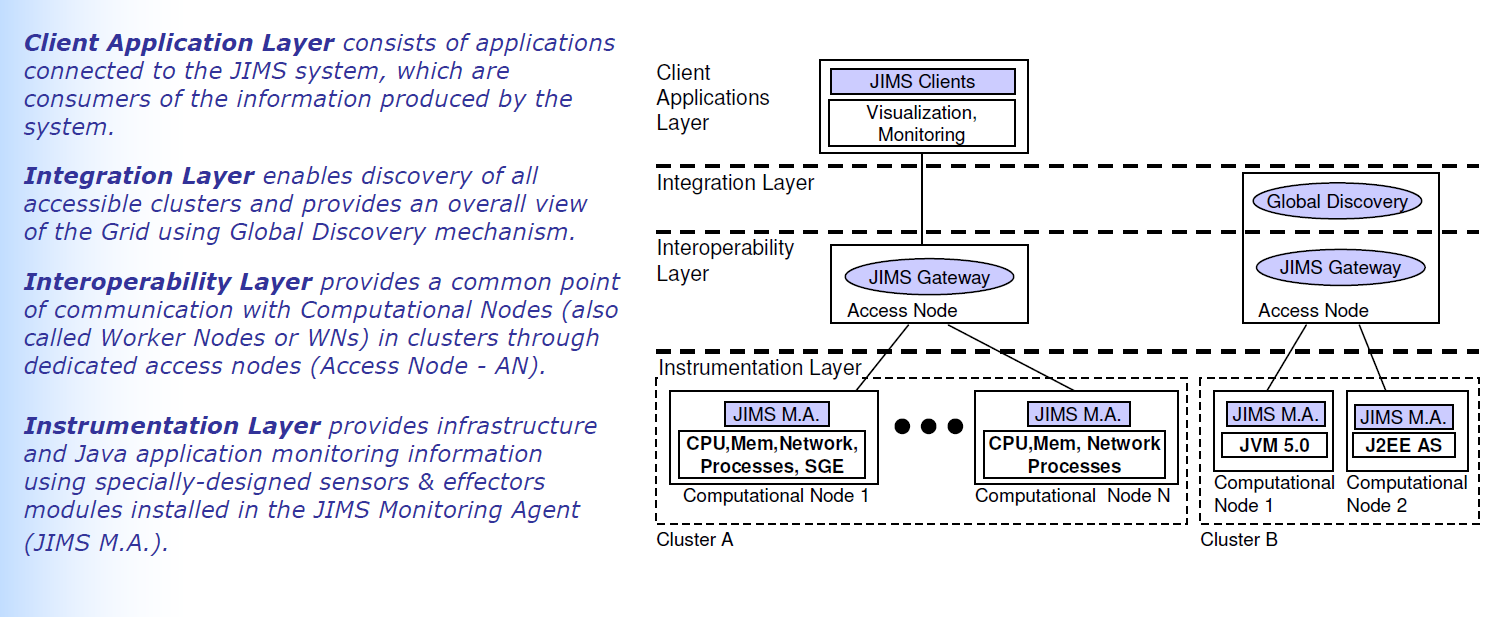
\includegraphics[width=0.9\textwidth]{img/jims/jims.png}
        \end{center}
        \caption{JIMS architecture \cite{jims}}
      \end{figure}

      The \gls{acr:jims} Extensions for Resource Monitoring and Management of Solaris 10 provides general architecture for
      monitoring and management applications written in Java.
	 
      Existing \gls{acr:jims} services enabling creating, reading and changing properties of Solaris zones are
      extensively used in the system during instantiating requested network structure.
    
     \subsection{The crossbow-gui implementation environment}

      \gls{acr:gui} application was developed in java using \gls{acr:swt} and swing graphic libraries. Project was managed with
      maven and thanks to maven profiles feature can be build and run on operating systems like:

      \begin{itemize}
        \item Solaris,
        \item Linux x86,
        \item Windows x86.
      \end{itemize}

      \gls{acr:swt} core libraries for these operating systems were provided in repository so the only requirements is to have
      one of the already mentioned operating system and installed: Java SE 1.6 or above and maven 2.x.
	  
	  \medskip
	  

      \section{The jims-crossbow-module implementation details}
	\label{sec:impl:module}
		
      To provide fully functional system allowing all expected functionalities new \gls{acr:jims} module called ''jims-crossbow-module'' was
      implemented. Created module consists of another three projects:

      \begin{itemize}
        \item Crossbow model components - performing crossbow like operations (\textbf{jims-crossbow-mbean}),
        \item Domain model transformation responsible for describing domain with actions (\textbf{jims-crossbow-model}),
        \item Infrastructure project for high-level management (\textbf{jims-crossbow-infrastructure}).
      \end{itemize}

      \begin{figure}[H]
        \centering
        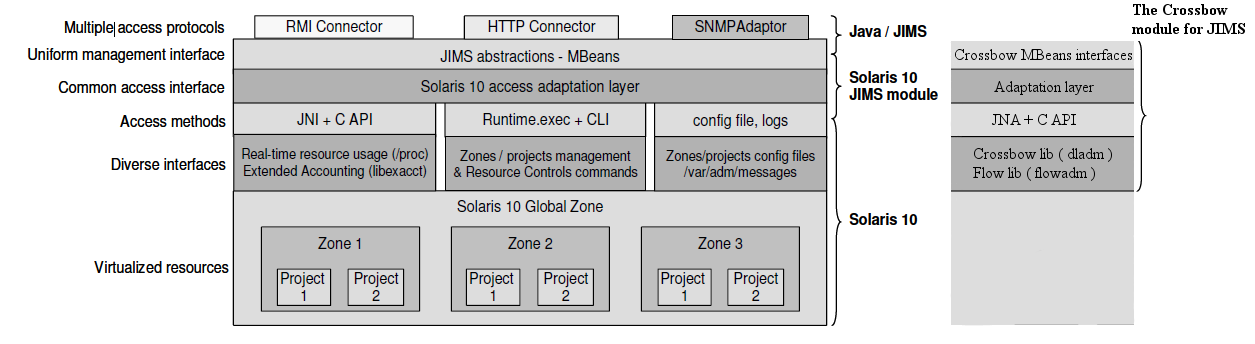
\includegraphics[width=1.26\textwidth, angle=90]{img/impl/jims_and_cm4j.png}

        \caption{The Crossbow module integrated with JIMS \cite{jims}}
      \end{figure}
		

      \subsection{Crossbow components implementation details}
      \label{sec:impl:comp}

        \begin{itemize}
          \item Plumb / unplumb operation, 
          \item Setting interface up or down operation,
          \item Reading and updating \gls{acr:mac}, \gls{acr:ip} address,
          \item Getting parent link name operation,
          \item Checking whether \gls{acr:vnic} was created under Etherstub or \gls{acr:nic},
          \item Reading / adding properties such as bandwidth limit, \gls{acr:vnic} packets priority.
        \end{itemize}

        As already mentioned each entities operation's are adjusted to their needs. Three figures \ref{fig:impl:etherstub}, 
        \ref{fig:impl:vnic}, \ref{fig:impl:flow} depict in detail each manager and its corresponding entity.


        \begin{figure}[H]
          \centering
          % TODO tikz
          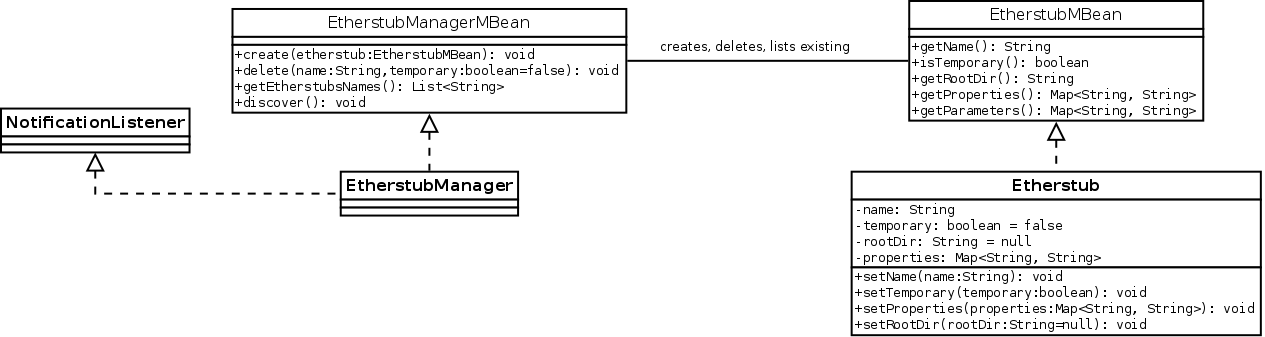
\includegraphics[width=1.2\textwidth, angle=90]{img/impl/etherstub.png}

	\label{fig:impl:etherstub}
          \caption{Etherstub class diagram}
        \end{figure}        

        \begin{figure}[H]
          \centering
          %TODO tikz
          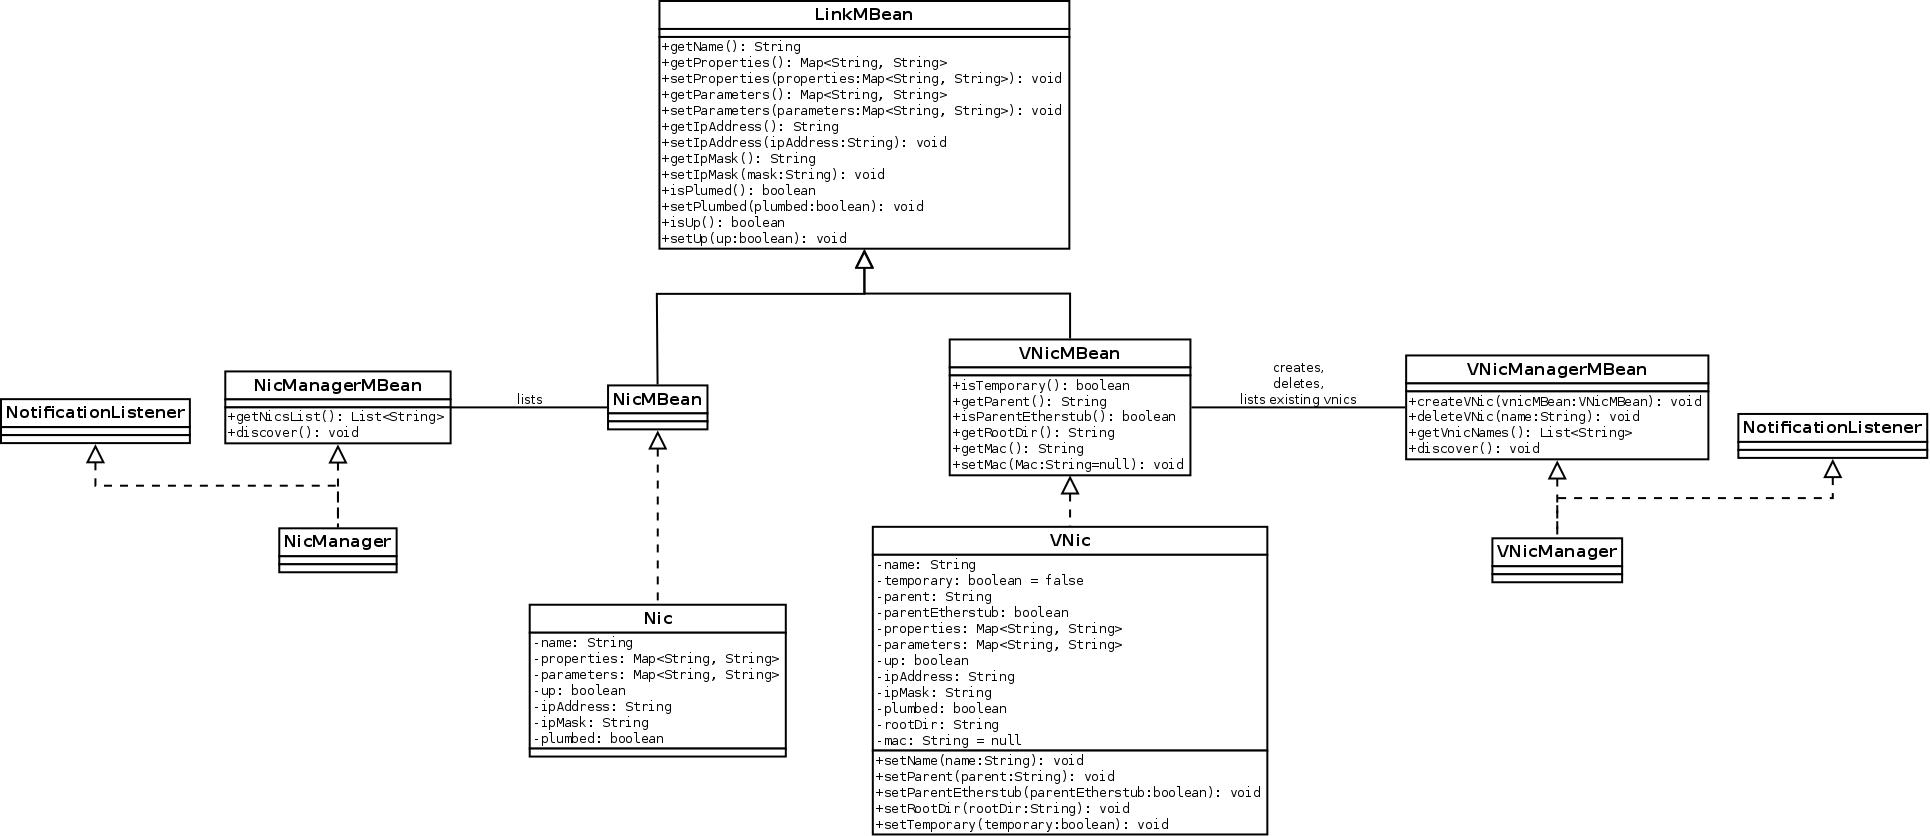
\includegraphics[width=1.2\textwidth, angle=90]{img/impl/link.png}

	\label{fig:impl:vnic}
          \caption{Link (VNIC, NIC) class diagram}
        \end{figure}        

        \begin{figure}[H]
          \centering
          % TODO tikz
          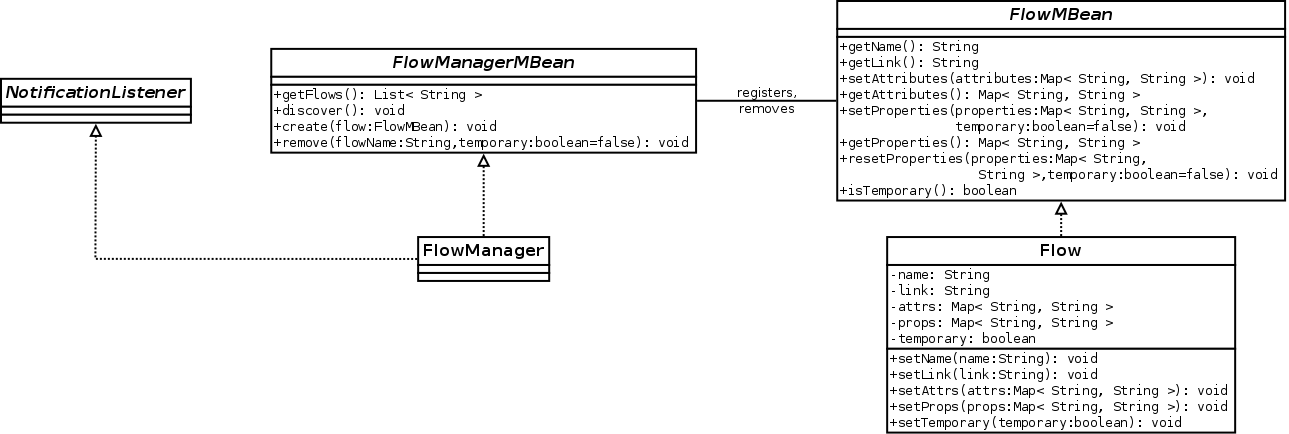
\includegraphics[width=1.2\textwidth, angle=90]{img/impl/flow.png}

	\label{fig:impl:flow}
          \caption{Flow class diagram}
        \end{figure}        

        Due to the fact that managers and entities have been separated and that each entity is an individual MBean
        these entities can be accessed not only from Java code but also be viewed and modified from JConsole.
		

      \subsection{Low-level functions access}
      \label{sec:impl:low}

        \gls{acr:jims} layered architecture together with crossbow dladm and flowadm library implicated the demand for 
        an approach towards accessing low-level functions.

        In developed application these approaches were adjusted to existing conditions so that for accessing functions
        from shared libraries \gls{acr:jna} was used and for doing more complex low-level operations shell scripts were
        written. Created jims-crossbow module contains shared library allowing
        \gls{acr:crud} operations which subsequently are being accessed by \gls{acr:jna}, whereas most of \gls{acr:jims}
        low-level access was done through running shell scripts. Although running scripts by ProcessBuilder is faster in implementation
        accessing native libraries through libraries like \gls{acr:jna} or \gls{acr:jni} gives more configurational advantage and does 
       not require shell script writing abilities.

        Listing \ref{lst:impl:low:jna} presents reduced example of \gls{acr:jna} access to native libraries. The
        corresponding native code in C language is shown in figure \ref{lst:impl:low:jnac}. \\


        \noindent
          \begin{minipage}{\textwidth}
          \lstinputlisting[caption={Native library access with JNA (Java code)},label={lst:impl:low:jna},language=Java]{lst/impl-jna.java}
        \end{minipage}  

        \noindent
        \begin{minipage}{\textwidth}
          \lstinputlisting[caption={Native library access with JNA (Native code)},label={lst:impl:low:jnac},language=C]{lst/impl-jna.c}
        \end{minipage}


      \subsection{Domain model transformations}
      \label{sec:impl:model}

        % TODO ta podsekcja dalej - za infrastructure project

        To allow conversion between network structure (as seen by the user in \gls{acr:gui} console) and underlying
        Crossbow components, a series of transformations is performed by Worker and Supervisor nodes. These
        transformations include simple one-to-one mappings as well as more sophisticated multi-step operations.
        In-depth description of the transformations follows together with a graphical example in figure
        \ref{fig:impl:transformation} \todo[inline]{narysowac}.

        % TODO obrazek!


        \subsubsection{Simple mappings}

          This is the class of transformations performed when instantiating or discovering abstractions that map
          directly to Crossbow components. These include switches, interfaces and policies. Worker component is
          responsible for performing the transformations. Table \ref{tab:impl:simple-mapping} contains detailed
          description of the mappings for each of the objects.

          \begin{table}[H]
            \centering

            \begin{tabularx}{\textwidth}{|c|c|X|}
              \hline
              Domain model class & Crossbow component & \centering Details \tabularnewline
              \hline \hline
              Switch             & Etherstub          & The simplest mapping; no attributes set \\
              \hline
              Interface          & \gls{acr:vnic}     & \gls{acr:vnic} created over \gls{acr:nic} or Etherstub \\
              \hline
              Interface          & \gls{acr:vlan}     & Logical \gls{acr:vlan}-specific interface; created when working
                                                        with routers connecting multiple physical nodes \\
              \hline
              Policy + Filter    & Flow               & The set of flow's attributes depends on the Filter specified;
                                                        Policy maps to Flow's properties \\
              \hline
            \end{tabularx}

            \caption{Domain model transformation (simple mappings)}
            \label{tab:impl:simple-mapping}
          \end{table}


        \subsubsection{Appliance to Zone transformation}

          It is necessary for network interfaces to be instantiated before a zone is created. For an Appliance to be
          fully instantiated, a sequence of steps is performed:

          \begin{enumerate}
            \item a proper snapshot is retrieved from appliance repository,
            \item the zone is configured --- network interfaces are attached,
            \item the zone is installed and booted,
            \item routing table is populated with user-defined entries.
          \end{enumerate}

          Appliances are discovered using the naming scheme --- all the zones in the system are inspected and only these
          matching the naming pattern are converted to the domain model entities. Then, for each of the discovered
          appliances, following steps are performed:

          \begin{enumerate}
            \item routing table entries are discovered,
            \item interfaces are attached (this is a part of Interface discovery process).
          \end{enumerate}


        \subsubsection{Routers connecting multiple Worker nodes}

          Topologies that embody different subnetworks and span multiple Worker hosts require special treatment ---
          traffic isolation has to be preserved and the network operation, from the end user's perspective, should be
          the same as for network deployed on a single physical machine. To satisfy these requirements, router zones
          with \gls{acr:vlan} interfaces are created on Worker nodes. The transformation is performed by Supervisor
          component: the object model is modified by duplicating the routing entity and enabling isolated communication
          channels for communication between physical hosts. Parts of the model are then sent to Worker nodes to finish
          the instantiation process (figure \ref{fig:impl:router}).

          \begin{figure}[h]
            \centering
            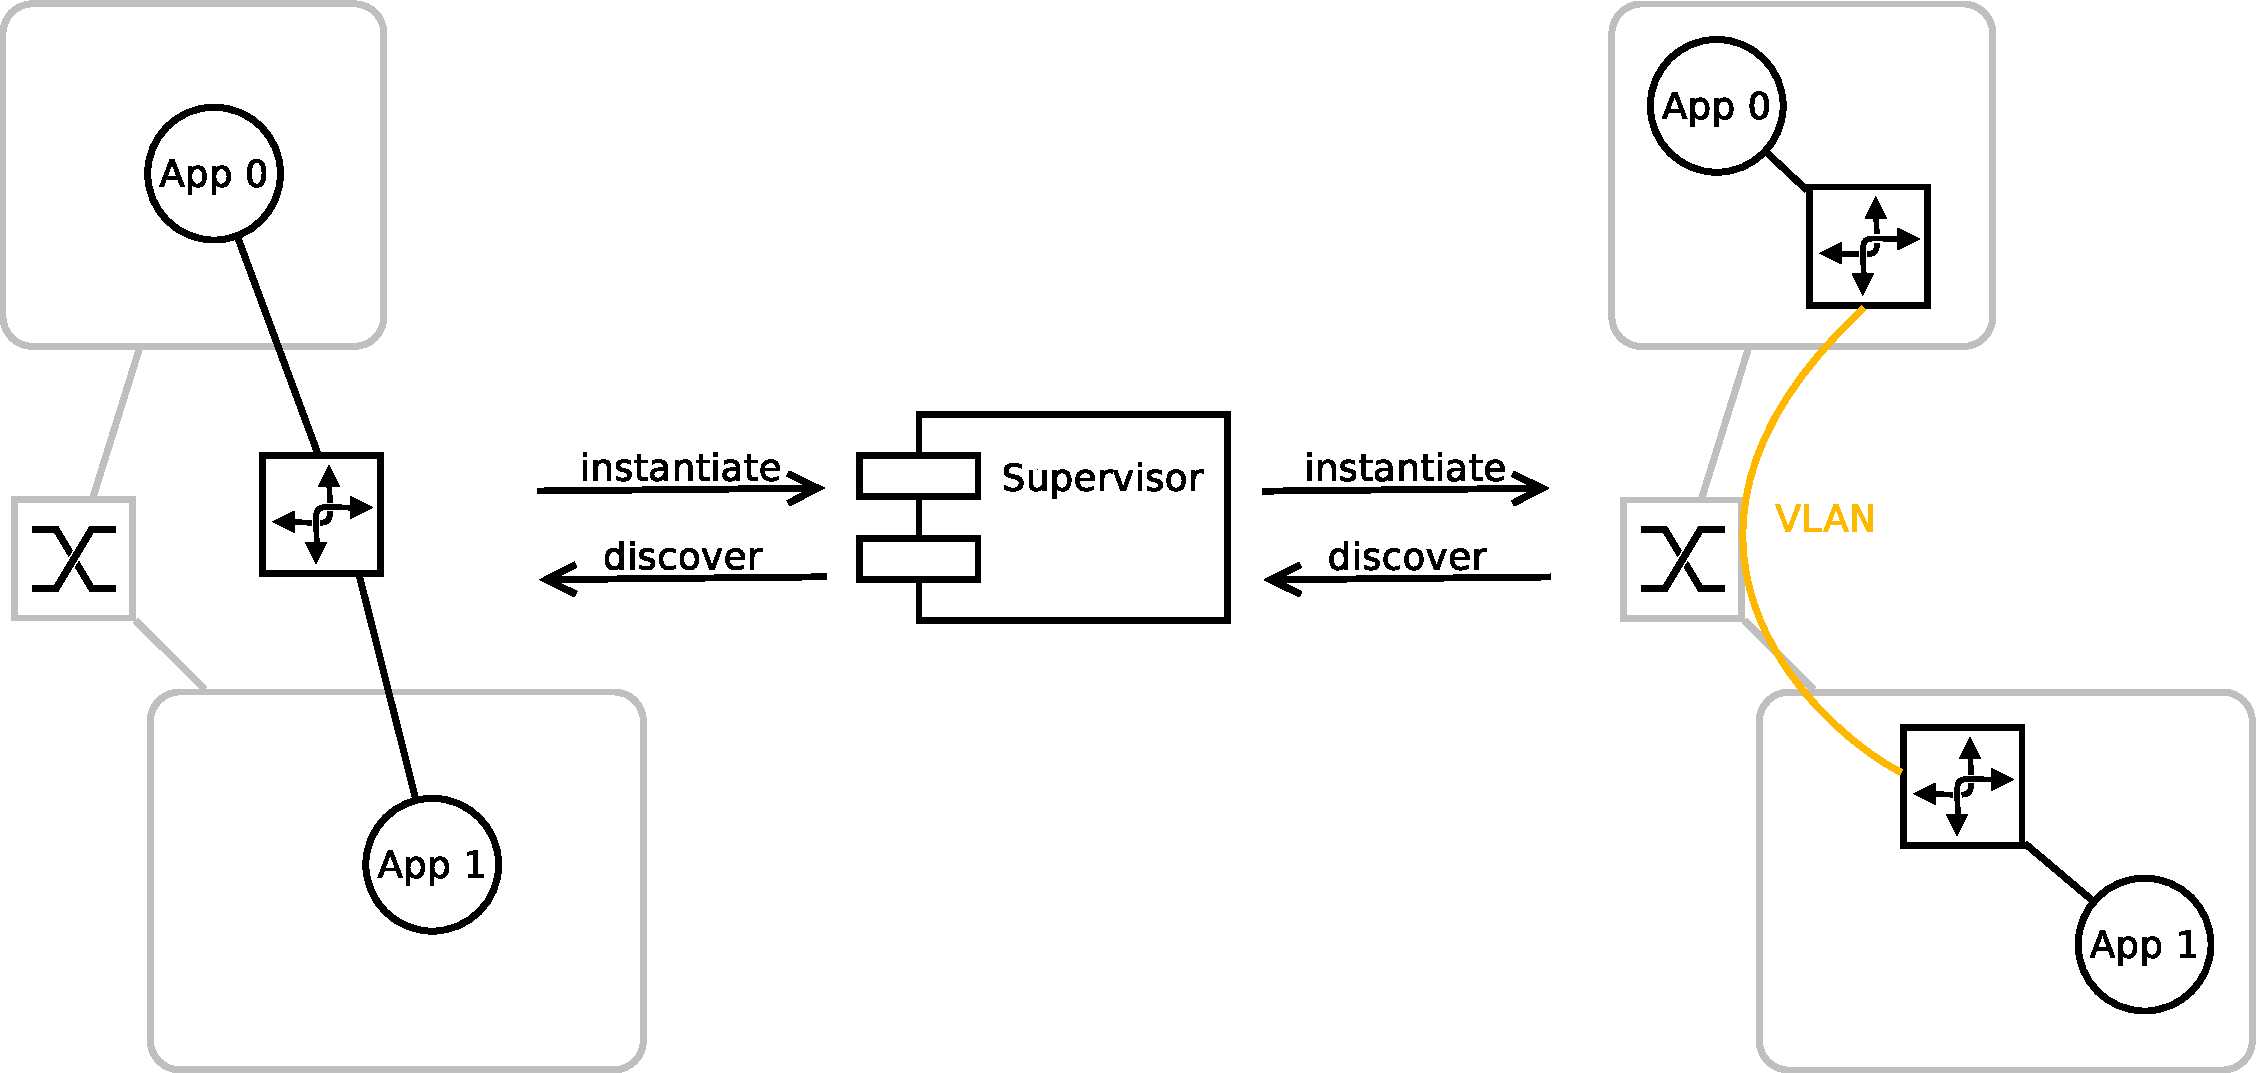
\includegraphics[width=.9\textwidth]{img/test-case/router.pdf}

            \caption{Internal model transformation for model spanning multiple nodes}
            \label{fig:impl:router}
          \end{figure}

          In the case of discovery, the steps are performed in reverse order --- Worker nodes discover, among others,
          router zones and \gls{acr:vlan} interfaces and send parts of the object model back to the Supervisor. The
          routers (together with routing tables) are merged to create single router entity that is placed in the object
          model. Auxiliary routers and \gls{acr:vlan} are then removed from the model.


      \subsection{Crossbow infrastructure project}
      \label{sec:impl:infrastructure}

        The jims-crossbow-module's subproject ( The Crossbow Infrastructure ) was designed in order to provide
        coarse operations like network structure instantiation, discovery, monitoring. 
        Functionalities provided by MBeans may invoked from \gls{acr:gui} console, JConsole or even from self written 
        applications by just adapting to existing interfaces and object names. 

        Existing high-level MBean are described and discussed in table \ref{tab:impl:hl-mbean}.

        \begin{table}[H]
          \centering

          \begin{tabular}{|l|l|p{4cm}|}
            \hline
            MBean                     & ObjectName                                  & Description                        \\
            \hline \hline
            SupervisorMBean           & \textbf{Crossbow:type=Supervisor}           & Main Bean runs whole instantiation
                                                                                      process (distributes model to
                                                                                      parts and passes them to proper
                                                                                      Worker                             \\
            \hline
            WorkerMBean               & \textbf{Crossbow:type=XBowWorker}           & Responsible for instantiating on
                                                                                      this node given model with regard
                                                                                      to specified  actions              \\
            \hline
            RepoManagerMBean          & \textbf{Crossbow:type=RepoManager}          & Allows getting/setting path to
                                                                                      projects placement, returns all
                                                                                      existing projects from working
                                                                                      path                               \\
            \hline
            StatisticGathererMBean    & \textbf{Crossbow:type=StatisticsGatherer}   & Provides statistics for interface
                                                                                      or flow for specified time period  \\
            \hline
            CrossbowNotificationMBean & \textbf{Crossbow:type=CrossbowNotification} & Returns progress of deployment,
                                                                                      logs with major information        \\
            \hline
          \end{tabular}

          \caption{High-level management MBeans}
          \label{tab:impl:hl-mbean}
        \end{table}
			
		
      \subsection{Data persistence}
      \label{sec:impl:persist}

        Although created system does not provide data persistence in databases, persistence in a bit unusual way  is
        provided. It is guaranteed on two levels: first is on \gls{acr:gui} level where user may save created
        network structure that is then serialized into file and second is on the \gls{acr:jims} nodes. During
        creation, discovery, removing network elements precise naming conventions are preserved. Due to this convention
        whole network is persistent and does not require any additional databases or files. Since generated names are
        complex, manual modification or creation of elements is not recommended as it is easy to introduce make to find
        errors --- created \gls{acr:gui} is provided for this purposes.

        With regard to statistics, flow's statistics are gathered and managed by operating system whereas \gls{acr:vnic}'s
        traffic load is gathered starting from every single \gls{acr:jims} restart.

        \begin{table}[H]
          \centering

          \begin{tabular}{|c|c|c|}
            \hline
            Domain model class & Solaris component & Naming scheme                                                \\
            \hline \hline
            Switch             & Etherstub         & \texttt{\{project\}\_S\{name\}}                              \\
            \hline
            Interface          & \gls{acr:vnic}    & \texttt{\{project\}\_\{appliance\}\_\{name\}}                \\
            \hline
            Policy             & Flow              & \texttt{\{project\}\_\{appliance\}\_\{interface\}\_\{name\}} \\
            \hline
            Appliance          & Zone              & \texttt{\{project\}\_M\{name\}}                              \\
            \hline
            Router             & Zone              & \texttt{\{project\}\_R\{name\}}                              \\
            \hline
          \end{tabular}

          \caption{Crossbow components naming scheme}
          \label{tab:impl:naming}
        \end{table}
		

      \subsection{System verification}
      \label{sec:impl:verif}
		
        Complexity of created system implies necessity of preparing tools verifying correctness of the system. In order
        to achieve this verification tests on each level of our system were prepared. Starting from (low-level) shared
        libraries, where unit tests for methods in C were implemented, through \gls{acr:jmx} level (with mocks)
        up to integration tests testing creating whole network structure. All prepared tests helped in finding most obvious
       mistakes and prepared system for testing with gui with lower risk of damaging underlying OS.  

      \section{GUI application}
      \label{sec:impl:gui}
		
        Developed \gls{acr:gui} application facilitates usage of the \gls{acr:jims} and newly implemented the jims-crossbow-module.
        Apart from project verification performed in the pre-instantiation stage, \gls{acr:gui} application is based on invoking 
        \gls{acr:jmx} Bean operation's and presenting received responses.

        Implemented \gls{acr:gui} application allows:

        \begin{itemize}
          \item Connecting to \gls{acr:jims} Gateway,
          \item Designing desired network structure with requested virtual appliances,
          \item Discovering and modifying already created projects,
          \item Detailed information about links and flows like bandwidth consumption presented in charts for requested
                time periods,
          \item Automatic logging using \gls{acr:ssh} to selected (already deployed) nodes and opening
                \gls{acr:gui}-like terminal emulator.
        \end{itemize}

        \begin{figure}[H]
          \centering
          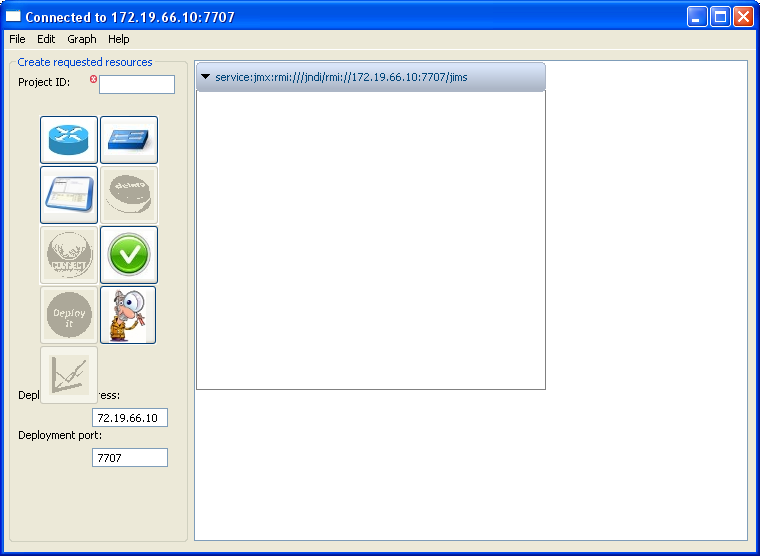
\includegraphics[width=0.7\textwidth]{img/impl/gui.png}

          \caption{GUI application}
        \end{figure}

        In relation to verification on the \gls{acr:gui} side of the system proper names, \gls{acr:ip} addresses, name duplicates and
        all necessary attributes are verified. Probability of future instantiation process failure is significantly reduces thanks to this verification, 
        although not totally prevented.

        \begin{figure}[H]
          \centering

          \begin{tikzpicture}[text height=1.5ex, text depth=.25ex]

            % TODO kosmetyka! review!

            \begin{umlseqdiag}

              \umlobject{GUI}
              \umlobject{Supervisor}
              \umlobject{ProgressShell}
              \umlobject{GraphToModelTranslator}
              \umlobject{CrossbowNotification}

              \begin{umlcall}[op={createActions(model, NetworkStructureHelper)}, return=Actions]{GUI}{GraphToModelTranslator}
              \end{umlcall}
              \begin{umlcall}[op={resetTotal(int numberOfNodes)}]{GUI}{CrossbowNotification}
              \end{umlcall}
              \begin{umlcall}[op={instantiate(model)}]{GUI}{Supervisor}
              \end{umlcall}
              \begin{umlcall}[op={open()}]{GUI}{ProgressShell}
                \begin{umlfragment}{type=loop, label={! deployed}}
                  \begin{umlcall}[op={getProgress()}, return={progress}]{ProgressShell}{CrossbowNotification}
                  \end{umlcall}
                  \begin{umlcall}[op={getNewLogs()}, return={logs}]{ProgressShell}{CrossbowNotification}
                  \end{umlcall}
                \end{umlfragment}
              \end{umlcall}

            \end{umlseqdiag}

          \end{tikzpicture}

          \caption{GUI side instantiation process}
        \end{figure}
		

    \section{Building and running the platform}
		\label{sec:impl:build}

      To build and run the platform the following prerequisites are required:

      \begin{itemize}
        \item Java SE 1.6, Maven,
        \item \gls{acr:jims} sources downloaded,
        \item jims-crossbow module\footnote{available at \url{https://github.com/robertboczek/solaris\-crossbow/tree/master/code}}
      \end{itemize}

      Afterwards \gls{acr:jims} project must be built. Detailed description of how to build \gls{acr:jims} is in README
      file located at the main directory of \gls{acr:jims} sources.

      Subsequently jims-crossbow module should be copied to the main folder containing \gls{acr:jims} and then build. The script
      inst-crossbow-lib.sh must be later executed to copy shared libraries *.so files to /usr/lib folder.

      If everything goes well, another step is running \gls{acr:jims}:

      \begin{itemize}
        \item \textit{jims-gateway: .../jims-gateway/bin/jims-agent.sh [-b host\_address] start | stop | restart},
        \item \textit{jims-agent: .../jims-agent/bin/jims-agent.sh [-b host\_address] start | stop | restart}.
      \end{itemize}

      On the main node just single jims-gateway should be run and on the remaining nodes as many jims-agents as it is
      required. For more information about \gls{acr:jims} and its architecture please refer to bibliography.

      If jims-agent or jims-gateway do not start, it is worth to see log files, located respectively at
      \textit{jims-agent/var/jims/log/agent.log} and \textit{jims-gateway/var/jims/log/agent.log}. 
      It is also  recommended to have the log file opened during \gls{acr:jims} start to see whether any exception was thrown 
      (\textit{tail -f jims\-gateway/var/jims/log/agent.log})

      \gls{acr:jims} has \gls{acr:jmx}-based architecture so each jims-agent and jims-gateway can be accessed through
      JConsole. In order to do that start JConsole, select remote process and enter type: \\
     \textit{service:jmx:rmi:///jndi/rmi://address:port/jims} where address and port is concrete
      address and port under which \gls{acr:jims} was started. The JConsole allows browsing registered mbeans and
      performing \gls{acr:crud} operations. Especially in case of the crossbow module it allows these operations as
      figure \ref{fig:impl:xbow-jconsole} presents.

      \begin{figure}[H]
        \centering
        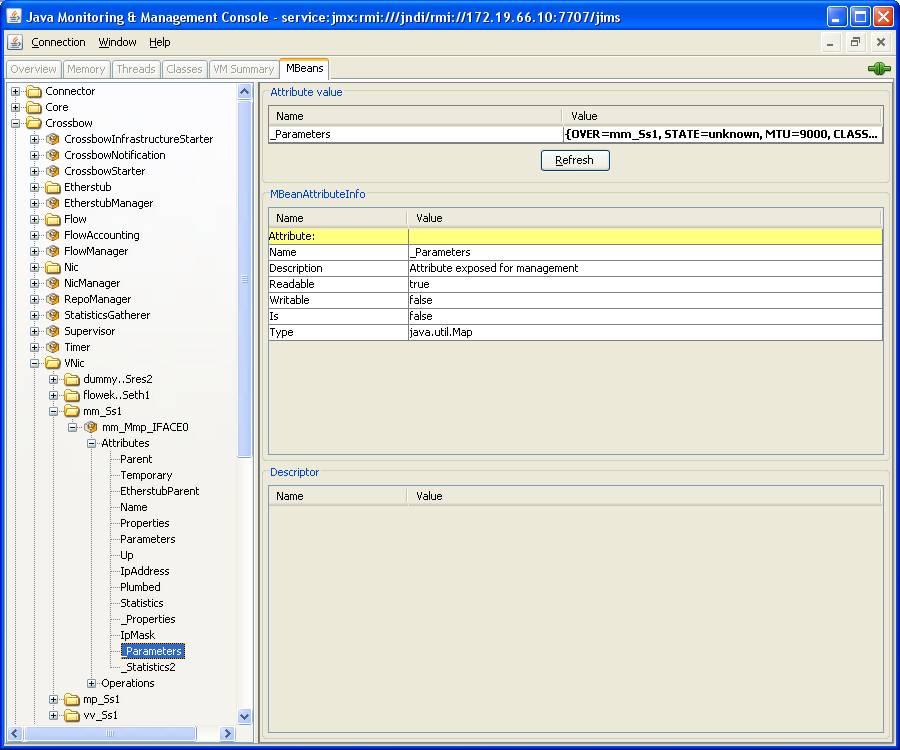
\includegraphics[width=1.0\textwidth]{img/impl/jconsole.png}

        \caption{The Crossbow module registered MBeans example}
        \label{fig:impl:xbow-jconsole}
      \end{figure}

      Building \gls{acr:gui}, which is located at 'jims/jims-crossbow/jims-crossbow-gui', requires Maven.
      Application may be imported to Eclipse and then built and run or built from console using Maven (\textit{mvn
      assembly:assembly}) and executed: \\
	\textit{java -cp target/jims-crossbow-gui-3.0.0-exe.jar org.jims.modules.crossbow.gui.Gui}.


    \section{Deployment issues}
    \label{sec:impl:problems}
		
		In terms of deployment, potential problems are easy to indicate. Use of \gls{acr:jims} functionality and related \gls{acr:jmx} 
		features stresses the lack of transactional support. Although in our system in case of errors introduced changes
		are usually removed, there is no guarantee that it will actually happen. Due to possible further errors caused during 
		restoring previous system state. In that case these partial changes must be removed manually from each node
		involved in this failing deployment attempt which generally imposes specialistic knowledge of underlying
		environment.


    \section*{Summary}
    \label{sec:impl:summary}

      This chapter introduced chosen approach to system implementation. Despite the fact that the requested functionalities
      were demanding and complex, the final product meets all the previously listed functional requirements. Thanks to used
      technologies such as \gls{acr:jmx}, the system with fully independent business layer (loosely coupled MBeans) was
      implemented. These technologies also helped to fulfill the defined non-functional requirements like: evolvability,
      extensibility, composability, etc. Definitely one of the biggest advantage of this system (apart from all
      the delivered functionalities provided by \gls{acr:cm4j}) is reusability as four possible usage models exist. The System may
      be managed from an implemented \gls{acr:gui}, a running JConsole or even from self developed (Java-based or native)
      application where developer can decide which part of \gls{acr:cm4j} would be used by just conforming to previously
      presented and described interfaces.


  \chapter{Case Study}
  \label{chap:cs}

    % TODO  dolozyc screen(y) z GUI

    The chapter describes the infrastructure that was built using the implemented system. Steps necessary to restore the
    configuration are listed and described. A number of tests were performed to evaluate the created system and
    topologies it allows to create. Resulting experimental data is presented and discussed.

    Section \ref{sec:uc:description} introduces the overall view of the topology that was created. Main components are
    described and \gls{acr:qos} requirements are discussed in more detail. Types of service are presented and
    appropriate network-level policies described. The policies are assigned to network components.

    Section \ref{sec:uc:prep} describes the stages needed to set up the topology. The steps include virtual appliance
    creation and publication, topology design, determining the quality policy and instantiation. Domain model of the
    designed topology and resulting low-level entities are listed.

    Section \ref{sec:uc:operation} presents the results of experiments performed to verify requirements the system has
    to meet. The section focuses on \gls{acr:qos}-related aspects --- it verifies definition, management and operation
    of the policies.

    Section \ref{sec:uc:enhance} lists the advantages of using the proposed system and approach to create, manage and
    monitor \gls{acr:qos}-aware virtual topologies. Aspects particularly helpful when preparing the case study are
    highlighted.

    Section \ref{sec:uc:eval} validates the system operation against defined requirements. All the major aspects of
    instantiation, discovery and monitoring processes are enumerated together with approaches chosen for \gls{acr:cm4j}
    design and implementation.


    \section{Scenario description}
    \label{sec:uc:description}

      The test case is inspired by multimedia systems. The problems of quality-aware transmission arise naturally in
      multimedia-oriented networks. Moreover, there are easily-identifiable classes of traffic with non-uniform quality
      requirements. This characteristics make multimedia networks a reasonable choice when considering tests focused on
      quality requirements verification.
      
      Also, complex topologies are built to enable multimedia transmission. The components that comprise these networks
      include, among others, specialized media servers, routers and client machines. This variety allows to demonstrate
      the usefulness of the created systems in the process of designing such topologies.


      \subsection{Types of service}
      
        As already stated, there are classes of traffic (or service types) that, by their nature, require different
        amounts of available resources (such as bandwidth, processing priority, etc.). The types of multimedia services
        map directly to \gls{acr:qos} policies required. Table \ref{tab:uc:qos} shows the mapping.

        \begin{table}[H]
          \begin{center}
            \begin{tabular}{|c|c|c|}
              \hline
              service type        & bandwidth & delay tolerance \\
              \hline \hline
              real-time streaming & high      & low \\
              \hline
              video on demand     & high      & high  \\
              \hline
            \end{tabular}
          \end{center}

          % TODO uzupelnic; czy zrodlo?

          \caption{Multimedia network traffic and its requirements}
          \label{tab:uc:qos}
        \end{table}

        The most demanding type of multimedia data is undoubtedly real-time streaming. The high priority data has to be
        favoured in order to provide desired level of quality --- precedence when accessing transport media and
        low-jitter transfer. This allows for low-delay streaming with small input data buffers on the client side.

        Video on demand data is of less priority. It is assumed that the user is not going to utilize the data as it is
        being downloaded. This assumption loosens the transmission requirements and allows to treat \gls{acr:vod}
        traffic as medium-priority or even best-effort data (no \gls{acr:cir}).


      \subsection{Topology overview}

        The network topology built is an attempt to model simple yet real environment used to transmit multimedia data.
        There is a streaming server without user differentiation mechanisms (with respect to quality of transmission)
        and an \gls{acr:http} server handling \gls{acr:vod} requests. The clients connect to the streaming server and
        start streaming sessions. They can also download video served by the \gls{acr:http} daemon.

        Client and server components are placed in different subnetworks that, in turn, are connected with a
        \gls{acr:qos}-aware router which provides one more level the policies can be defined at. Rules defined for the
        router's interfaces specify fine-grained policies for clients in subnetworks in addition to the ones defined at
        the server level.

        Taking this approach, it is easy to enable \gls{acr:qos}-aware networking leveraging relatively simple
        applications. The aspects of choosing server and client implementations and providing quality of service become
        orthogonal and the whole design remains clear and maintainable. Figure \ref{fig:cs:scenario} presents an
        overview of the network structure and client configuration.
      
        \begin{figure}[H]
          \begin{center}
            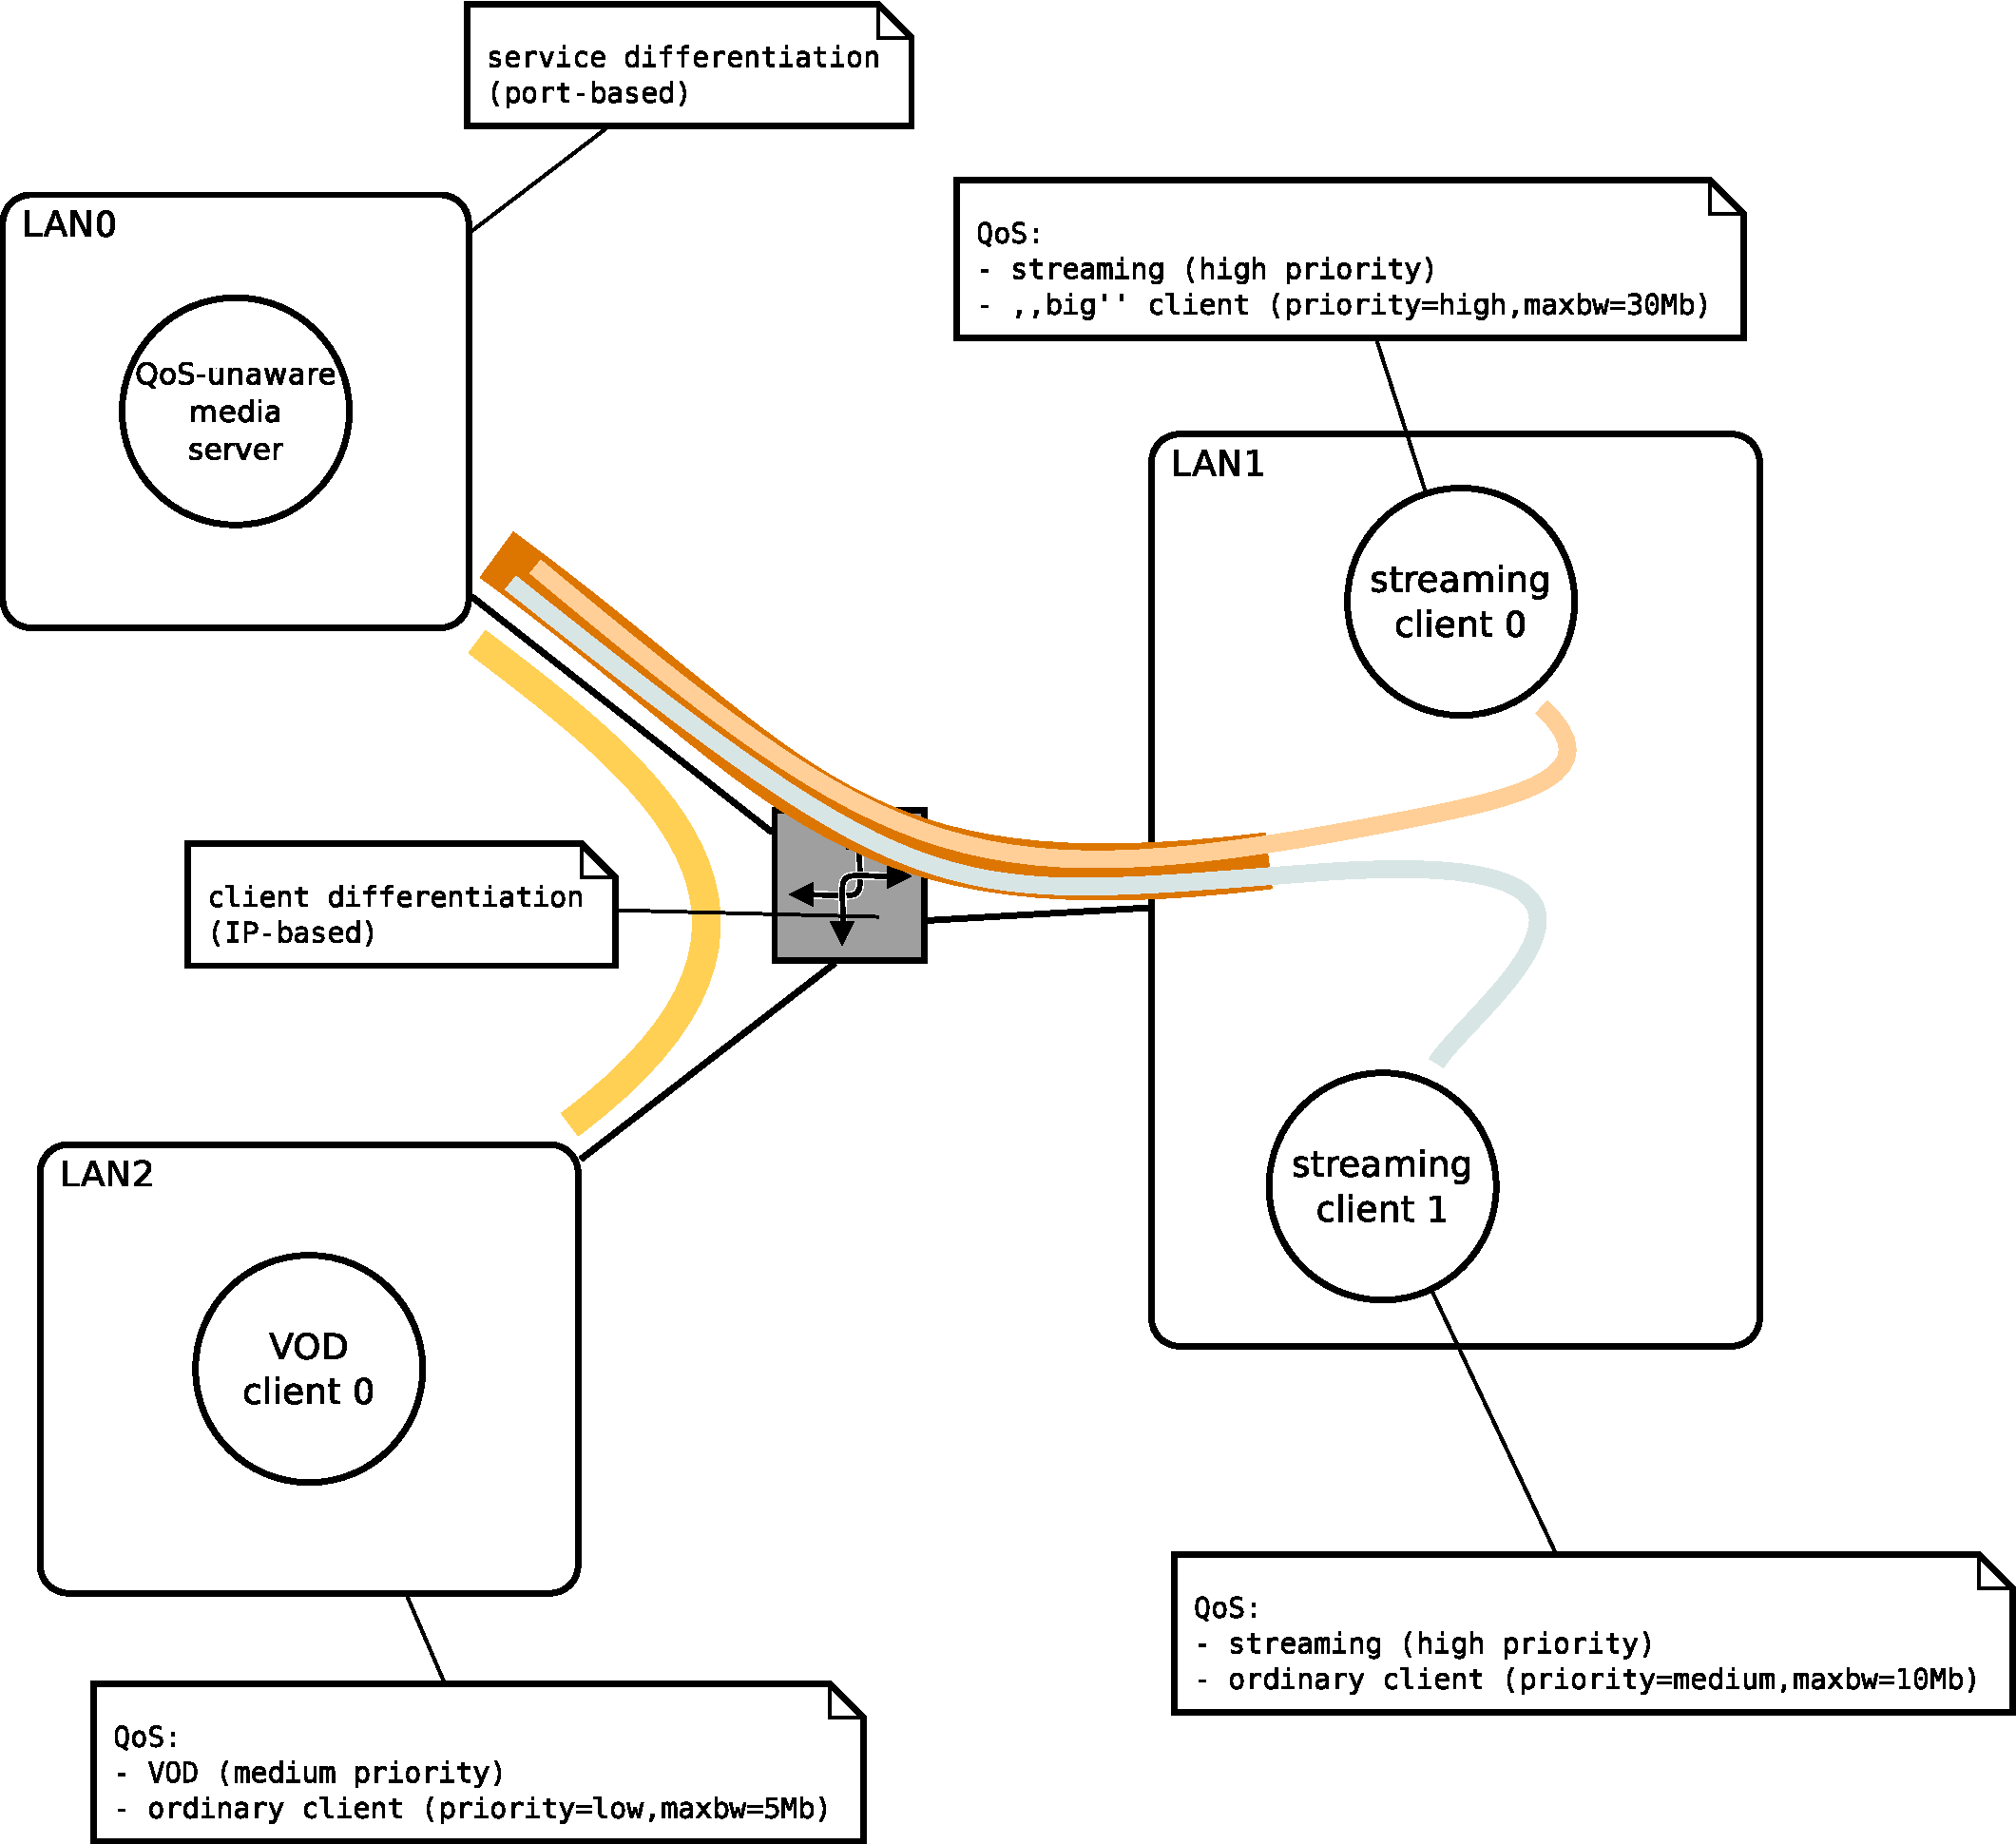
\includegraphics[width=0.8\textwidth]{img/test-case/diagram.pdf}
          \end{center}

          \caption{High-level view of the created topology}
          \label{fig:cs:scenario}
        \end{figure}
      

      \subsection{Service and client differentiation}
      \label{sub:uc:diff}

        The traffic is classified based on two properties: type of service (\gls{acr:rtp}, \gls{acr:http}) and recipient
        address. Three traffic classes are distinguished with respect to service type:

        \begin{itemize}

          \item high priority \gls{acr:rtp} streaming

                UDP traffic with source ports 6970 and 6971, used by streaming client 0
                and streaming client 1 in LAN1 subnetwork,

          \item low priority Video On Demand
          
                TCP traffic with source port 80, used by the \gls{acr:vod} client 0,

          \item medium priority ordinary traffic
          
                all the other data.

        \end{itemize}

        Furthermore, the streaming clients inside the LAN1 subnetwork are assigned different priority values. Client 0
        is favoured and has high priority for \gls{acr:rtp} data, whereas client 1 is assigned low priority. Client 0 in
        LAN2 is not assigned any priority explicitly.


    \section{Preparation of the environment}
    \label{sec:uc:prep}

      General steps while building the environment are: virtual appliance preparation, topology design and
      instantiation. Virtual appliances are created manually and published in an \gls{acr:nfs} repository. Then, they
      are used as building blocks when designing the network. Finally, the virtual infrastructure is designed and
      instantiated (using the \gls{acr:gui} frontend), i.e.  all the underlying low-level components, like zones,
      etherstubs, \gls{acr:vnic}s and flows, are created.


      \subsection{Virtual appliances}
      \label{ssub:case:prep:va}

        Listing \ref{lst:uc:prep:create} shows the initial steps when creating new zones. In this case, the zone is
        called \texttt{mplayer} and it contains a streaming client. At first, new ZFS pool is created to host the zone's
        filesystem, then basic configuration is performed and the zone is installed. \\

        \noindent
        \begin{minipage}{\textwidth}
          \lstinputlisting[caption={New zone creation},label={lst:uc:prep:create}]{lst/uc-create.sh}
        \end{minipage}

        \noindent
        It may be necessary to modify \texttt{/etc/shadow} file as in listing \ref{lst:uc:prep:sed} to be able to access
        the zone with \texttt{zlogin}. \\

        \noindent
        \begin{minipage}{\textwidth}
          \lstinputlisting[caption={\texttt{/etc/shadow} file adjustment},label={lst:uc:prep:sed}]{lst/uc-sed.sh}
        \end{minipage}

        \noindent
        After installation the zone can be booted and used after logging (listing \ref{lst:uc:prep:boot}). \\

        \noindent
        \begin{minipage}{\textwidth}
          \lstinputlisting[caption={Booting and logging into a zone},label={lst:uc:prep:boot}]{lst/uc-boot.sh}
        \end{minipage}

        \noindent
        All the required software should be installed now. When the zone is prepared, a ZFS snapshot can be taken and
        transferred to the repository (listing \ref{lst:uc:prep:snap}). \\

        \noindent
        \begin{minipage}{\textwidth}
          \lstinputlisting[caption={Publishing a snapshot in NFS repository},label={lst:uc:prep:snap}]{lst/uc-snap.sh}
        \end{minipage}


      \subsection{Topology instantiation}
      \label{ssub:}

        After all necessary virtual appliances have been created and stored in the repository, network topology can be
        designed and instantiated. Following steps comprise the whole process:

        \begin{enumerate}
          \item selection of virtual appliance templates from the repository,
          \item designation of physical machine(s) to host the topology,
          \item appliance-to-host assignment,
          \item enabling network connection between nodes, addressing, routing setup,
          \item defining \gls{acr:qos} policies.
        \end{enumerate}

        The topology consists of router (forwards \gls{acr:ip} packets between its directly-attached interfaces), server
        (with Darwin Streaming Server and thttpd \gls{acr:http} server installed) and client appliances (mplayer
        compiled with \gls{acr:rtp} streaming support enabled). All the appliances are instantiated on a single physical
        host.

        There are three subnetworks:

        \begin{itemize}
          \item 1.1.1.0/24 contains only the server appliance (addressed 1.1.1.2),
          \item 2.2.2.0/24 with one \gls{acr:vod} client (addressed 2.2.2.2),
          \item 3.3.3.0/24 with two streaming clients (addressed 3.3.3.2 and 3.3.3.3).
        \end{itemize}

        The router appliance, with three interfaces (addressed 1.1.1.1, 2.2.2.1 and 3.3.3.1) links the subnetworks and
        provides network-level connectivity. Each of the appliances has additional entries in its routing table.

        \gls{acr:qos} assurance is composed of two main stages:

        \begin{itemize}
          \item bandwidth of the links used to stream and download media is limited to 8Mbps (mainly to make the
                testing process easier),
          \item traffic is divided into classes and policies are assigned to the classes.
        \end{itemize}

        Service differentiation is based on local port numbers and users are differentiated with respect to their
        network addresses. To achieve this, PortFilter and IpFilter are applied. PortFilter specifies a triple
        \mbox{(port number, location, protocol)} --- the example for \gls{acr:rtp} is \mbox{(6970, LOCAL, UDP)}.
        IpFilter specifies a triple \mbox{(\gls{acr:ip} address, netmask, location)} --- the example for a client in
        1.1.1.0/24 subnetwork is \mbox{(1.1.1.2, 24, REMOTE)}.

        Relative bandwidth assignment is achieved with priorities. The PriorityPolicy instances determining traffic
        priority (LOW, MEDIUM, HIGH) have to be applied to specific interfaces.

        Figure \ref{fig:cs:topo} presents the complete topology built with domain model elements. It includes virtual
        appliances (:Machine, :Router), connectivity (:Interface, :IpAddress, :Switch), policies (:PriorityPolicy,
        :BandwidthPolicy) and filters (:PortFilter, :IpFilter).

        \begin{figure}[H]
          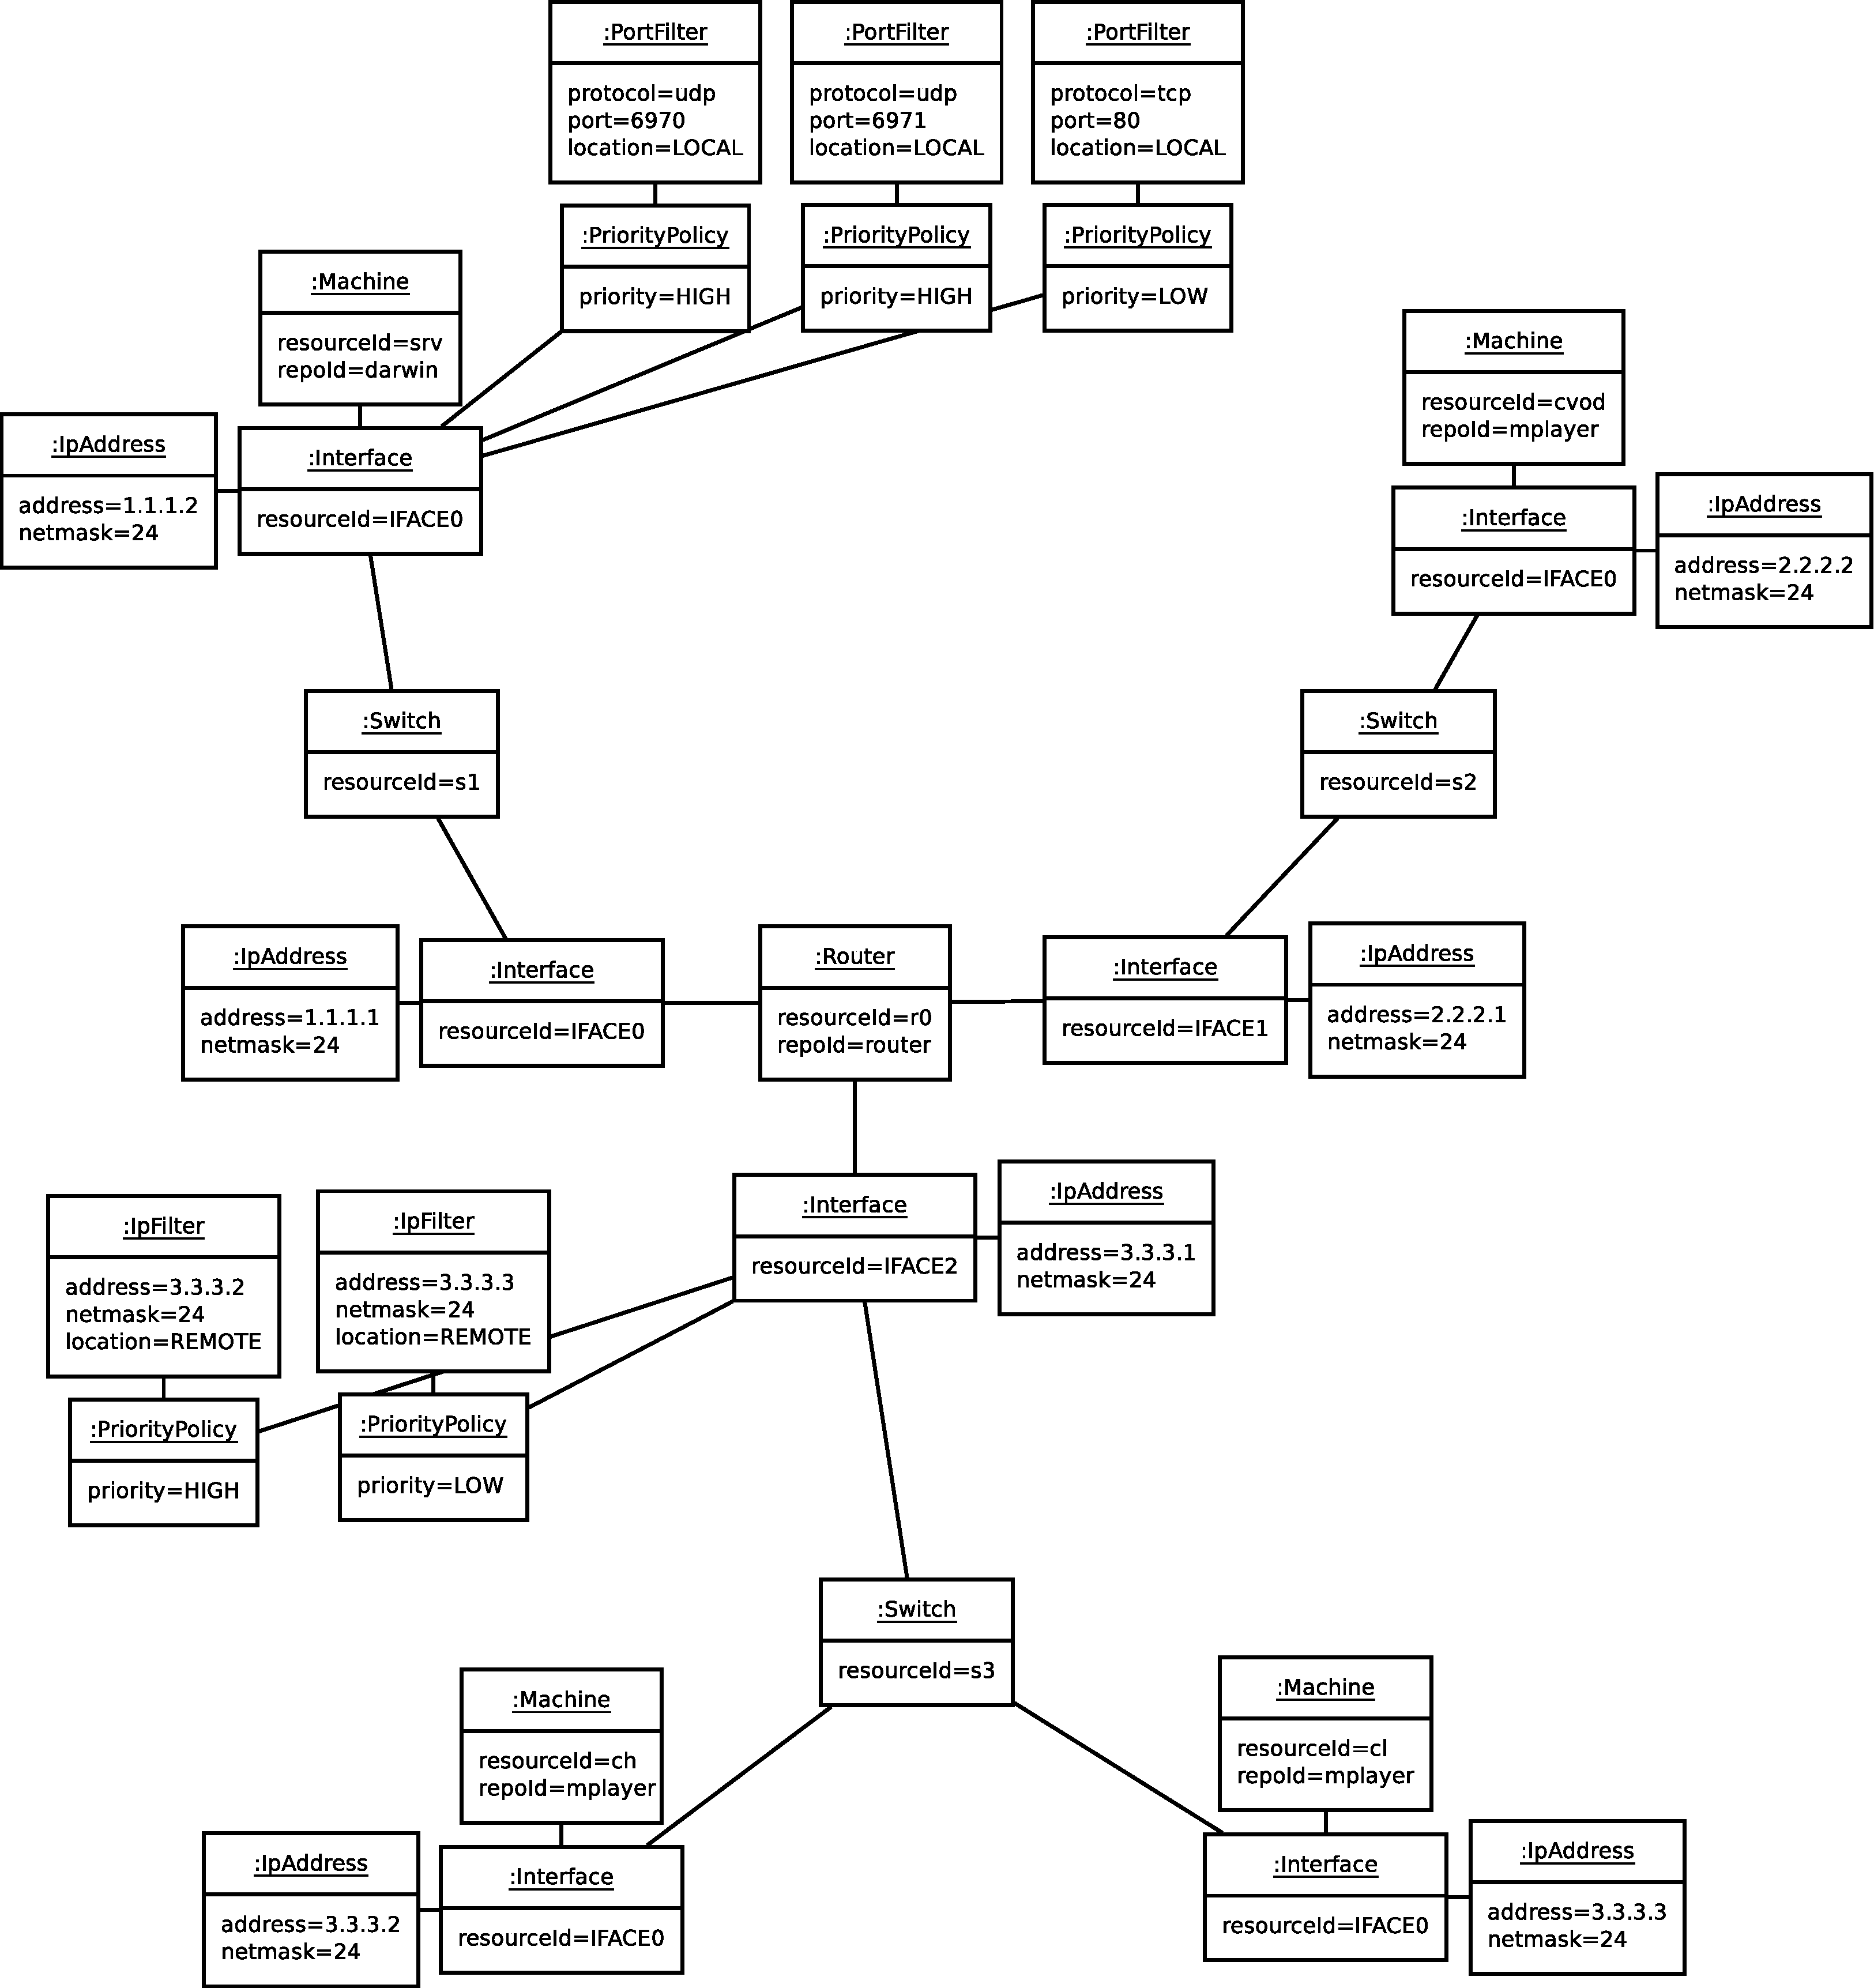
\includegraphics[width=.9\textwidth]{img/test-case/topology-om.pdf}

          \caption{Network topology expressed in terms of the domain model}
          \label{fig:cs:topo}
        \end{figure}

        % TODO ^ maxbw!
      
      
      \subsection{Resulting Crossbow and Solaris components}
      \label{sub:uc:xbow}

        A successful model instantiation creates a number of Crossbow and Solaris entities. The resulting set contains
        zones, etherstubs, \gls{acr:vnic}s and flows that reflect the desired configuration. These entities work together and
        provide fully operational network topology.

        All the entity names follow the same pattern --- they are prepended with project identifier (\texttt{uc\_}).
        There are five zones created, as shown in listing \ref{lst:uc:xbow:zone} (one media server, three clients and
        one router). \\

        \noindent
        \begin{minipage}{\textwidth}
          \lstinputlisting[caption={All the zones created after model instantiation},label={lst:uc:xbow:zone}]{lst/uc-zone.sh}
        \end{minipage}

        Each of the zones has virtual interfaces (\gls{acr:vnic}s) assigned. Flows are created for some of the interfaces. The
        server zone and all of the client zones are connected to the router zone with etherstubs. Listing
        \ref{lst:uc:xbow:ether} enumerates the etherstubs, \gls{acr:vnic}s and flows are shown in listing \ref{lst:uc:xbow:vnic} \\

        \noindent
        \begin{minipage}{\textwidth}
          \lstinputlisting[caption={Etherstubs},label={lst:uc:xbow:ether}]{lst/uc-ether.sh}
        \end{minipage}

        \noindent
        \begin{minipage}{\textwidth}
          \lstinputlisting[caption={Virtual interfaces and flows created on top of them},label={lst:uc:xbow:vnic}]{lst/uc-vnic.sh}
        \end{minipage}

        Figure \ref{fig:cs:topo-xbow} shows the interconnections between resulting Crossbow components. Colors
        correspond to these in figure \ref{fig:cs:topo}.

        \begin{figure}[H]
          \centering
          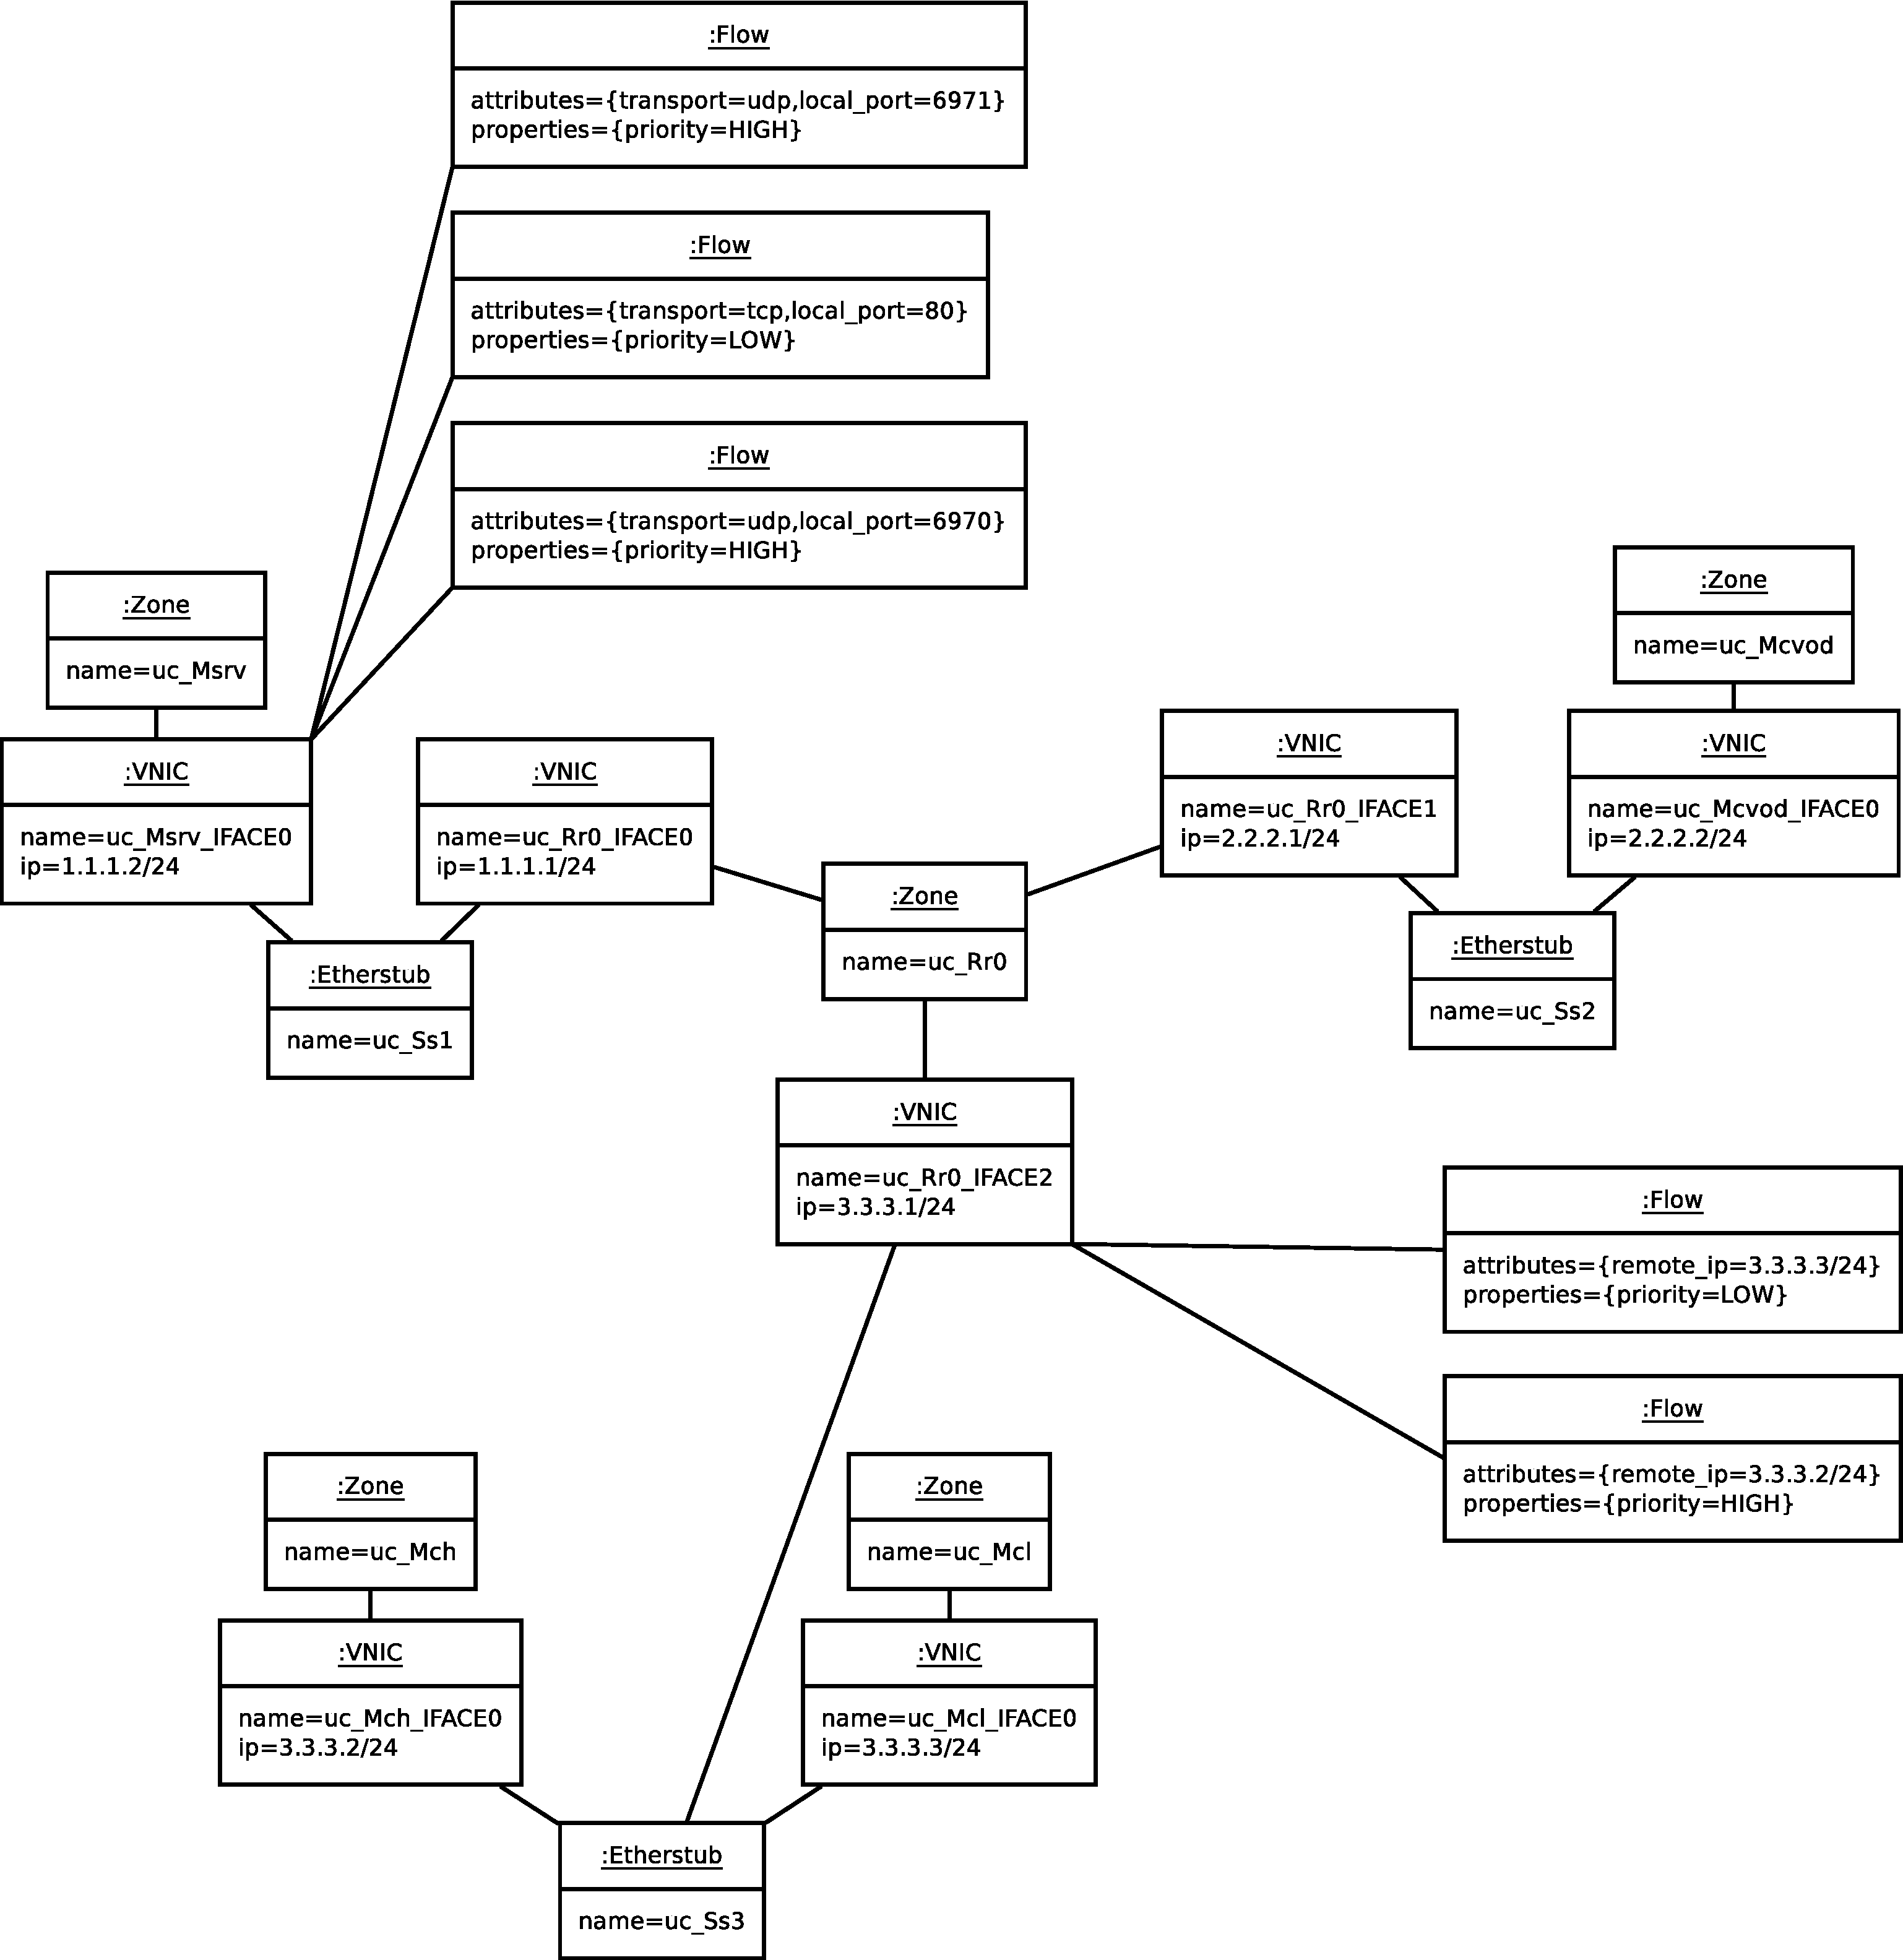
\includegraphics[width=.9\textwidth]{img/test-case/topology-xbow.pdf}

          \caption{Network topology transformed to Solaris components}
          \label{fig:cs:topo-xbow}
        \end{figure}


      \subsection{Media preparation}
      \label{sub:}

        For a movie to be streamed, hint tracks have to be created. Hints are meta-data that provide information on how
        to stream audio and video tracks. This information is then used by the server when dividing the media into
        packets and sending them via the network.

        The sequence of commands in listing \ref{lst:uc:media:prep} demonstrates how to prepare a movie to be streamed
        by Darwin Streaming Server (the example leverages ffmpeg\footnote{available at \url{http://www.ffmpeg.org}} and
        mpeg4ip\footnote{available at \url{http://mpeg4ip.sourceforge.net}} utilities). First, the data streams are
        transcoded to MPEG4 (video) and \gls{acr:aac} formats and saved in an MPEG4 container. Then, hint tracks are
        appended to the container. \\

        \noindent
        \begin{minipage}{\textwidth}
          \lstinputlisting[caption={Media preparation before streaming},label={lst:uc:media:prep}]{lst/uc-prep.sh}
        \end{minipage}


    \section{The infrastructure operation}
    \label{sec:uc:operation}

      \tikzstyle{chart-label}=[text depth=.25ex]

      The traffic data is gathered as follows: each host node has tshark utility installed. It is set up to monitor all
      the traffic on the server interface and write it to a file (as shown in listing \ref{lst:uc:op:tshark}). When the
      gathering process is finished, the data is handed to wireshark and analyzed - graphs with throughput values are
      generated to show the interdependencies between the streams of data. \\

      \noindent
      \begin{minipage}{\textwidth}
        \lstinputlisting[caption={Monitoring network traffic with tshark},label={lst:uc:op:tshark}]{lst/uc-tshark.sh}
      \end{minipage}

      The tests include verifying that the set up bandwidth limitations work on per-client basis, different service
      types are treated according to the policy and streaming client differentiation requirements are satisfied. The
      main metric used is bandwidth each of the streams is assigned.


      \subsection{Limiting the bandwidth}
      \label{sub:uc:limit}

        Bandwidth is limited to 8Mbps for all the links. The limits can be changed online with immediate effects. Figure
        \ref{fig:uc:limit} shows bandwidth limitation for a \gls{acr:vod} client downloading a movie. After a short
        period of transmission rate limited to 24Mbps, the link bandwidth is narrowed to 8Mbps (lowest supported value).

        \begin{figure}[H]
          \centering

          \begin{tikzpicture}[node distance=0]
            \node (img) at (0,0) {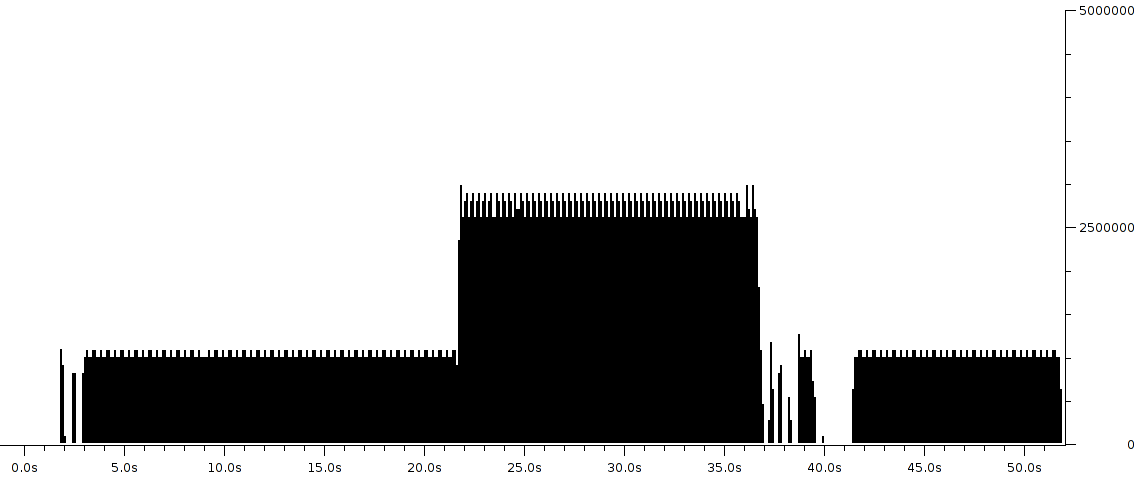
\includegraphics[width=.7\textwidth]{img/test-case/limit.png}};
            \node [below=of img.south west] {time $[\mathrm{s}]$};

            \useasboundingbox (current bounding box);

            \node [right=of img.north east] {bandwidth $[\mathrm{MB}/\mathrm{s}]$};
          \end{tikzpicture}

          \caption{8Mbps bandwidth limitation}
          \label{fig:uc:limit}
        \end{figure}


      \subsection{Policies for different types of traffic}
      \label{sub:uc:traffic}

        A \gls{acr:vod} client is downloading a long movie. All the bandwidth is available. Another client connects to the
        streaming server and requests a number of video streams. As the \gls{acr:rtp} data is of high priority, the streaming
        client is favoured over \gls{acr:vod} client and it gets most of the available bandwidth.

        \begin{figure}[H]
          \centering

          \begin{tikzpicture}[node distance=0]
            \node (img) at (0,0) {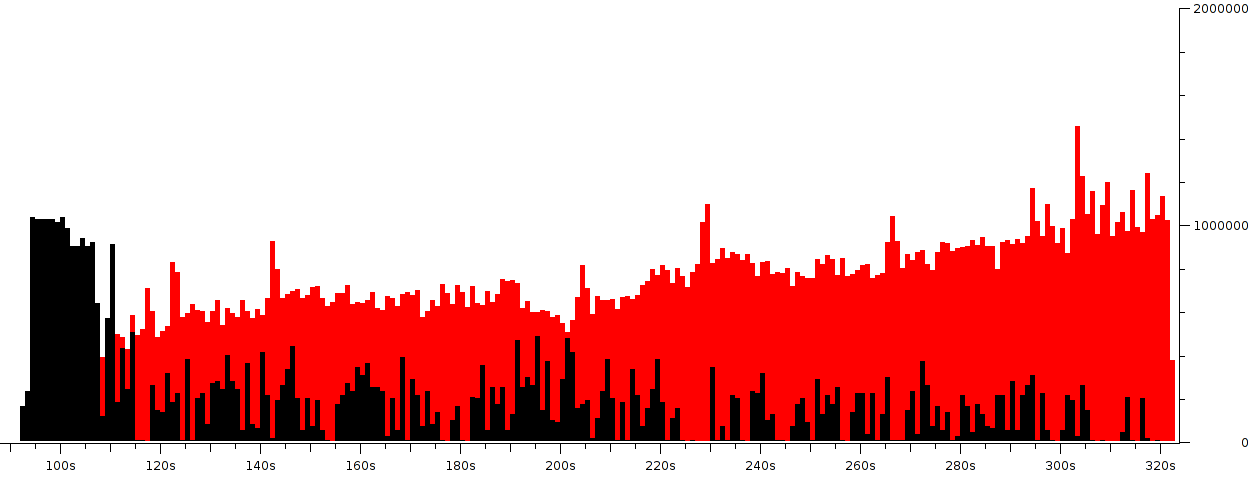
\includegraphics[width=.7\textwidth]{img/test-case/vod-rtp.png}};
            \node [below=of img.south west] {time $[\mathrm{s}]$};

            \node (rtp)  [below=of img.north west, anchor=north west, shape=rectangle, fill=red] {}; \node (rtp-label)  [right=of rtp, chart-label]  {RTP};
            \node (http) [below=.2cm of rtp, shape=rectangle, fill=black]                        {}; \node (http-label) [right=of http, chart-label] {VOD};

            \useasboundingbox (current bounding box);

            \node [right=of img.north east] {bandwidth $[\mathrm{MB}/\mathrm{s}]$};
          \end{tikzpicture}

          \caption{VOD traffic bandwidth consumption compared to high-priority RTP streams}
        \end{figure}


      \subsection{Client-dependent quality of service}
      \label{sub:uc:client}

        A \gls{acr:vod} client is downloading a movie. Two clients connect to the streaming server and request a number
        of video streams. One of the streaming clients has low priority assigned, the other one is high priority.
        \gls{acr:rtp} streaming gets most of the bandwidth and high priority client is favoured over the low priority
        one.

        \begin{figure}[H]
          \centering

          \begin{tikzpicture}[node distance=0]
            \node (img) at (0,0) {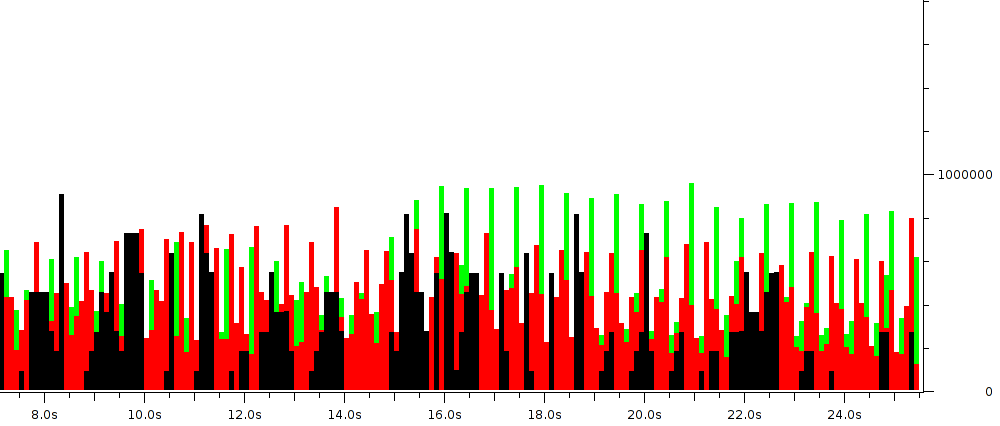
\includegraphics[width=.7\textwidth]{img/test-case/exp-all.png}};
            \node [below=of img.south west] {time $[\mathrm{s}]$};

            \node (rtp-hp) [below=of img.north west, anchor=north west, shape=rectangle, fill=green] {}; \node (rtp-hp-label) [right=of rtp-hp, chart-label] {high-priority RTP};
            \node (rtp-lp) [below=.2cm of rtp-hp, shape=rectangle, fill=red]                         {}; \node (rtp-lp-label) [right=of rtp-lp, chart-label] {low-priority RTP};
            \node (vod)    [below=.2cm of rtp-lp, shape=rectangle, fill=black]                       {}; \node (vod-label)    [right=of vod, chart-label]    {VOD};

            \useasboundingbox (current bounding box);

            \node [right=of img.north east] {bandwidth $[\mathrm{MB}/\mathrm{s}]$};
          \end{tikzpicture}

          \caption{Distribution of available bandwidth between streaming clients}
        \end{figure}


    \section{Enhancements provided by the solution}
    \label{sec:uc:enhance}

      The implemented system provides extensive support for most of the stages that comprise virtual network management.
      There are two main goals the system is designed to achieve: to limit the time spent by the administrator to create
      and manage the topology and to make the process as intuitive as possible.


      \subsection{Topology design}
      \label{sub:uc:enhance:design}

        The \gls{acr:gui} console displays the topology in the form of a graph --- with virtual appliances (or switches) as nodes
        and connections as edges. With this approach it is easy to visualize the structure of the network so that it can
        be quickly understood and adjusted.

        All the essential aspects of the network design are configurable with \gls{acr:gui} wizards. The system provides an easy
        way to set up addressing, routing and quality policies. Also, appliance repository access is integrated. Input
        data describing the model is validated while being entered by the user. 


      \subsection{Infrastructure instantiation}
      \label{sub:uc:enhance:instantiation}

        By automating the instantiation process (ie. snapshot retrieval and transfer, zone attachment and configuration)
        a lot of user's time is saved. This does not only cover the time required to log in to a host system and enter
        commands manually --- the instantiation stages, when possible, are performed concurrently and can save
        significant amount of time required by this process.

        Input validation minimizes the risk of mistakes, especially when big topologies are considered and the whole
        design becomes complicated. A consistent naming scheme is provided so that the topology can be managed when the
        system is not available.

        % TODO progress bar, czy tutaj, czy w implementacji?
        % TODO nawiazanie do deploymentu z va (chapter: solaris)


      \subsection{Online modifications}
      \label{sub:uc:enhance:online}

        With online modification support it is easy to adjust the system without breaking its operation. The quality
        policies, for example, already instantiated can be changed, whenever needed.

        Even more sophisticated control is possible. For example, additional rule-based component could be developed and
        integrated with the system to allow automatic adjustment based on statistical data.


      \subsection{Monitoring}
      \label{sub:uc:enhance:monitoring}

        Historical data can be accessed. There are customizable usage charts that can display bandwidth usage for
        policies and interfaces. Also, load on the host machine can be monitored to help designer assess which machines
        to choose when assigning the appliances.


    \section{Evaluation results}
    \label{sec:uc:eval}

      The case study confirmed the completeness of the implemented system with respect to requirements identified. All
      major groups of functional requirements --- instantiation, discovery, monitoring --- were verified while working
      with the topology under test.

      The complete topology together with \gls{acr:qos} policies was created with the \gls{acr:gui} console provided.
      The console supports the user throughout the processes of design, instantiation, discovery, monitoring and
      adjustment. Graph network representation used by the \gls{acr:gui} proved to be intuitive and allow easy
      management of complex networking structures.

      Total deployment time could be substantially reduced thanks to virtual appliances. Created snapshots were
      published in a repository accessible from the \gls{acr:gui} console and became reusable building blocks of complex
      topologies, minimizing the number of repetitive tasks administrator would have to perform otherwise.

      The graph view user is presented maps directly to general, implementation-independent domain object model.
      Internal model transformations and model instantiation itself were verified to be correct. Also, the inverse
      process of discovery was tested --- input topology was restored using only data persisted in target operating
      system.

      As the \gls{acr:cm4j} does not use database for data persistence, topology adjustment using non-\gls{acr:gui}
      tools may seem to be challenging. However, thanks to clear and consistent naming scheme, experienced user is able
      to tweak an existing topology manually, using utilities provided by the operating system.

      Created topologies fulfill the requirements of isolation and traffic differentiation that respects defined
      \gls{acr:qos} policies. This is achieved thanks to Crossbow technology itself as well as carefully designed object
      model transformations.

      Resulting infrastructure can be managed in a multitude of ways. Low-level components are accessible with command
      line utilities provided by the Crossbow project (flowadm, dladm) and with higher-level native \gls{acr:api}
      developed as a part of the thesis. Also, \gls{acr:jmx} objects instrumenting Crossbow entities are exposed to
      allow easy integration with Java platform. Finally, the infrastructure, expressed in terms of the domain model,
      can be retrieved using the Supervisor component and manipulated with \gls{acr:gui} console.

      Although the topology presented in the chapter is complex, it does not take advantage of all the functionalities
      implemented. Creation of even more sophisticated designs (like topologies spanning multiple physical nodes with
      \gls{acr:qos} policies and still preserving traffic isolation) is possible with \gls{acr:cm4j}.


    \section*{Summary}

      The chapter presented all the steps that were undertaken to ensure the system meets the identified requirements.
      The ability to create and manage complex network topologies was demonstrated by designing and instantiating
      a multimedia oriented network with a wide variety of components used. Validity and operation of deployed
      infrastructure was confirmed by the tests performed. It was shown that communication between virtual appliances is
      possible with properly configured routing tables. And, most importantly, the experiments confirmed that
      the \gls{acr:qos} policies are preserved.


  \chapter{Summary}
  \label{chap:sum}

	  The chapter summarizes the outcome of the research conducted in the area of network virtualization with special regard to 
	  the proposed thesis statement.
	
	  Section \ref{sub:sum:concl} briefly concludes the research results and the test-case results. The thesis statement's legitimacy and feasibility 
	  is also discussed in this section. All the accomplished goals and objectives are outlined in section \ref{sub:sum:achieved}, yet
	  possible improvements that might be introduced to the created system are considered in section \ref{sub:sum:further}.

    \section{Conclusions}
		\label{sub:sum:concl}
		
      The statement proposed at the beginning of the thesis claming that: \emph{There exists a layered architecture which
      enables the construction of a system that would facilitate working with a fully iisolated virtualized network and
      resources grouped by project name} was deeply considered throughout this thesis by the authors.  In order to
      fulfil the proposed statement a detailed requirement analysis was performed. Subsequently in order to comply with all
      the defined requirements mentioned in the thesis statement the layered architectural approach was chosen. This approach
      allowed to distinguish certain groups of independent, highly cohesive components. Together these components create
      the planned system, but each one could be used separately allowing to perform operations like: \gls{acr:crud}
      operations over virtual network elements, virtual resources management, etc. 
      
      The investigation performed while working on this paper allowed the authors to understand the concepts of a complex network
      virtualization and resource reservation principles and sharing in more details. The conducted tests additionally outlined the
      significance of these issues and proved how important they are in terms of success of proper work of complex systems.
      Encountered problems only confirmed that although very useful they are also demanding and require a comprehensive
      knowledge in a variety of computer areas. 

      
    \section{Achieved goals}
		\label{sub:sum:achieved}

      % TODO o tym, ze cos sie nie udalo, bym stad wywalil do nastepnej sekcji
		
      In relation to the achieved goals not all were unfortunately successfully finished. Time shortage and the lack of people
      did not allow for as deep an insight at this issue as was initially planned. However, some objectives are really
      worth to be mentioned:
      
      \begin{itemize}
        \item Significant improvements in system configuration in comparison to manual setup,
        \item Automatic update of given network parameters,
        \item Reusability provided thanks to loosely coupled components hidden under well defined interfaces,
        \item Presenting network topology in a clear and natural way (graph format).
      \end{itemize}
		
      Hopefully the presented system and the whole concept of network virtualization, resource allocation and isolation 
	    would encourage the reader to do his own research in this area.
		

    \section{Further work}
		\label{sub:sum:further}
	
      There are many welcomed improvements that may be added to the \gls{acr:cm4j} system. Probably the largest
      component initially planned was an automatic resource assigner that would run and perform automatic resource
      assignments to nodes that run under the lowest load. This assigner with an attached rule-based system would gather data
      about the load on each node and based on that it would decide what and where to instantiate.  Unfortunately, the presented and discussed
      system in this thesis lacks that functionality. Instead, it offers manual assignments, where user selects on which
      node new virtual resources should be created. Another functionality not implemented, yet welcomed would be a semi-automatic
      snapshot creation. Currently a user can create Solaris zone from existing snapshot and use it. The functionality where
      the created resource could be converted to snapshot and then transferred to the repository would definitely improve
      the system's usability.

      \todo[inline]{wiecej}


  \printglossaries

  \bibliographystyle{plain}
  \bibliography{bibliography}


\end{document}

% vim: et : tw=120 : spelllang=en_us,pl : spell :





